\chapter{Application of convolutional neural networks for CHIPS} %%%%%%%%%%%%%%%%%%%%%%%%%%%%%%%%%
\label{chap:cvn} %%%%%%%%%%%%%%%%%%%%%%%%%%%%%%%%%%%%%%%%%%%%%%%%%%%%%%%%%%%%%%%%%%%%%%%%%%%%%%%%%

TELL THEM WHAT YOU ARE GOING TO TELL THEM WITH A TOUCH OF MOTIVATION

The principal goal of any physics analysis and no different for \chips, is the correct
classification of signal events and the rejection of background events. Also of great importance
is the accurate estimation of the energies of the particles involves in the interaction.

Traditionally hand-engineered features and simple machine learning models have been used for
classification of events and kinematic methods have been used for energy reconstruction.

Water Cherenkov detectors generate essentially an `image' of the neutrino interaction and
therefore they are well suited to use things from computer vision.

- Core of any particle physics analysis is the selection of signal events.
- Traditionally hand-engineered features extracted from event reconstruction are passed to a
machine learning algorithm for classification.
- Want an approach that relies less on event reconstruction, preferable using the raw detector
outputs as input.

- Core problem in experiment HEP is the correct categorisation of the particle interactions
recorded in out detectors as either signal or background.
- Commonly/typically this is done by reconstructing high level components such as clusters,
tracks, showers, jets, and rings associated with the particle interactions. And then summarising
the energies, directions etc.... of these objects.
- Prone to failings, mistakes in the reco of high level features from the raw data can lead to
incorrect categorisation.
- Features then used to categorise events are limited to those which have been imagined and then
implemented for the specific experiment.
- This problem shares many similarities with the problems of computer vision. With great advances
being made to move away from specially constructed features to the extraction of features using
convolutional neural networks.

- The principle goal of event reconstruction in CHIPS is to identify electron neutrino
interactions against a large background of muon neutrinos and NC interactions.
- Explain the goals of both event reconstruction and event classification/ particle identification
- Main purpose for now is to allow for the exploration of different detector designs, for future
CHIPS detectors.

- CNNs have been widely applied in various computer vision tasks to solve image recognition and
analysis problems.
- Many HEP problems including water cherenkov detectors essentially result in an 'image' of an
event, which are well suited to these tools.
- MLP are widely used in HEP,
- Deep neural networks have emerged as one of the most powerful supervised learning techniques.

- If one photon has a much lower energy than the other, or they are very closely overlapped,
they are commonly misidentified as a single electron.
- The shape of the ring can then be used for particle identification
- Muon rings tend to be sharper and exhibit a `plateau' shape as they emmit a constant amount of
Cherenkov radiation from a single particle over a period of time.
- Electron rings are more diffuse due to their production being from a electromagnetic shower.

- In this chapter I will outline the current implementations used by \chips
- Then I will give theoretical context to the deep learning methods
- Then I will discuss the implementation to \chips and the process through which the optimal
was found.
- Then I will discuss the conslusions.
- Can be split into regression and classification tasks
- Present a convolutional neural network for cosmic muon rejection, beam event classification and
neutrino energy estimation.

\section{Previous applications of deep learning to neutrino experiments} %%%%%%%%%%%%%%%%%%%%%%%%
\label{sec:cvn_previous} %%%%%%%%%%%%%%%%%%%%%%%%%%%%%%%%%%%%%%%%%%%%%%%%%%%%%%%%%%%%%%%%%%%%%%%%%

Over the last few years, neutrino experiments have started to adopt various deep learning
techniques for a range of tasks. This trend has generally followed the explosion of interest in
the field amongst the global research community, especially in computer vision, as can be seen in
Fig.~\ref{fig:papers}.

\begin{figure} % NUMBER OF PAPERS DIAGRAM DIAGRAM %
    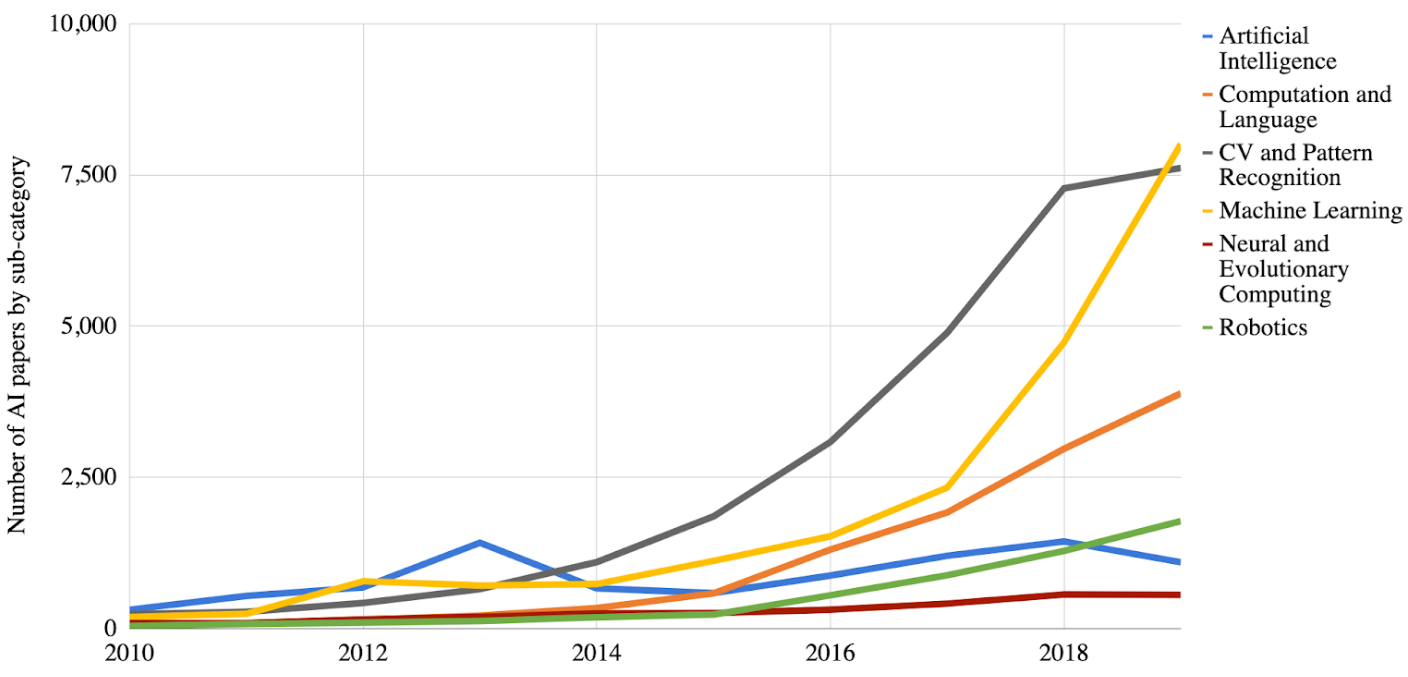
\includegraphics[width=0.8\textwidth]{diagrams/7-cvn/papers.png}
    \caption[papers short]
    {The number of artificial intelligence papers submitted to arXiv, broken down by sub-category.
        Note the particularly large increase in Computer Vision (CV) and pattern recognition
        papers. Figure taken from Ref.\cite{perrault2019}.}
    \label{fig:papers}
\end{figure}

In 2016 the \nova experiment initially applied a convolutional neural network to the task of
classifying the interaction type of events within their sampling calorimeter
detector~\cite{aurisano2016}. Two views of raw detector events were used as input to train a
network based on the popular GoogLeNet architecture~\cite{szegedy2015}, discussed in section
\ref{sec:cvn_theory_architectures}. An improved iteration of the network has since been applied to
both the classification of individual clusters of energy deposits~\cite{aurisano2016} and the
regression task of electron neutrino and electron energy reconstruction.

Convolutional neural networks have also been applied to liquid argon time-projection chambers. The
MicroBooNE experiment has shown that in addition to classification tasks, the localisation of
single particles within events is possible~\cite{acciarri2017}. Furthermore, the DUNE
collaboration has designed a network to output both the interaction type and counts of the
different types of particle in an event~\cite{collaboration2020, abi2020}. This approach is called
multi-task learning, which will be discussed in greater detail in \ref{sec:cvn_baseline_multi}.

Applications to water Cherenkov detectors have also been made, by both the Daya Bay reactor
experiment~\cite{racah2016} and the KM3NeT/ORCA collaboration~\cite{aiello2020}. Additionally, a
type of generative network known as a `variational autoencoder' has been shown to approximate the
distribution of simulated water Cherenkov data~\cite{abhishek2019}. If further studies prove
successful, this could allow for training on real data to reduce experimental uncertainties and
increase the speed of data generation by many orders of magnitude.

\section{Standard event reconstruction and classification} %%%%%%%%%%%%%%%%%%%%%%%%%%%%%%%%%%%%%%%
\label{sec:cvn_old} %%%%%%%%%%%%%%%%%%%%%%%%%%%%%%%%%%%%%%%%%%%%%%%%%%%%%%%%%%%%%%%%%%%%%%%%%%%%%%

It is essential to outline the standard event reconstruction, and classification methods that have
been used by the \chips project for detector optimisation studies up till now. This is key for two
main reasons. Firstly, to add context when comparing the new convolutional neural network approach
as is done later in the chapter. Secondly, to highlight the main weaknesses of these methods,
motivating the new technique and making its advantages clear.

A maximum likelihood method based on that implemented by MiniBooNE~\cite{patterson2009} is used
for event reconstruction. Additionally, an artificial neural network built using the TMVA
package~\cite{hocker2007} and using outputs from the reconstruction, is used for event
classification. Both methods are very typical of the `mainstream' approach used by the majority of
water Cherenkov neutrino experiments. A prime example is the fiTQun algorithm developed for the
Super-Kamiokande detector, which is now used for both atmospheric~\cite{jiang2019} and
T2K~\cite{missert2017} analyses.

Due to the small size and limited resources of the \chips project collaboration, it is highly
likely that both the event reconstruction and classification do not represent the `optimal'
implementation of these methods. However, through tracking the development process of both
methods, it is clear that any performance improvements would now be small relative to those
introduced by the new convolutional neural network approach. Thus, it can be assumed that the
implementation approximates the maximum performance these approaches can provide reasonably well.

\subsection{Likelihood based reconstruction} %%%%%%%%%%%%%%%%%%%%%%%%%%%%%%%%%%%%%%%%%%%%%%%%%%%%%
\label{sec:cvn_old_reco} %%%%%%%%%%%%%%%%%%%%%%%%%%%%%%%%%%%%%%%%%%%%%%%%%%%%%%%%%%%%%%%%%%%%%%%%%

The event reconstruction methodology is simple in theory: for a given set of hypothesised tracks,
the number of photoelectrons and the time at which the first of these is recorded for each PMT in
the detector is predicted. By comparing this prediction with the measured hit charges and times
the likelihood that the given track hypothesis produced the measured signals can be calculated.
The parameters that describe the hypothesised tracks are then varied until the negative logarithm
of the likelihood is minimised. Identifying the best-fit parameters for the hypothesis. A brief
description of the full procedure is given below, however, for a full description see
Ref.~\cite{blake2016} and in great detail Ref.~\cite{perch2017}.

The first stage of event reconstruction is the effective seeding of tracks that are then used in
the full likelihood fit. The seeding methods aim to provide a good starting point for the
minimisation, both to increase the efficiency of finding the optimal track parameters and also to
avoid a false local minimum from being returned.

Firstly, the PMT hits are sliced in both space and time. Gaps in the time ordering of hits are
used to separate the event into time slices. Each of these then undergoes basic filtering and
clustering to remove outlying hits and ensure only the dominant collections of hits are
considered. Each cleaned slice is then run through simple vertex finding algorithms to estimate
the interaction position and time, as well and the initial track direction.

A circular Hough transform algorithm, traditionally used for water Cherenkov ring finding is then
applied. The voting-based transformation produces as output a space within which rings of PMT hits
exist as single peaks. The track direction values are then further refined using this space, and a
search for smaller peaks is carried out to indicate if multiple particles are likely to be
involved. This process results in a list of seeds with a corresponding score related directly to
the height of the associated peak in Hough transform space.

Each track in a fit hypothesis is made up of a vector of parameters $\vec{x}$, containing the
following:
\begin{itemize}
    \item The track vertex position ($x_{0}$, $y_{0}$, $z_{0}$) and interaction time $t_{0}$.
    \item The initial track direction ($d_{\theta}$, $d_{\phi}$).
    \item The initial kinetic energy of the particle.
    \item The particle type (muon, electron or photon).
\end{itemize}
Additionally, for a photon hypothesis (identical to an electron hypothesis in reality) the
distance between the interaction vertex and the beginning of the electromagnetic shower initiated
by the $\gamma$ is included as a parameter.

These parameters are then initialised using the parameters found in the seeding procedure in
descending order of Hough peak height score. As the particle energy is not estimated by the
seeding algorithms, a default value equal to the average particle energy observed in the Monte
Carlo simulation is assigned. Additionally, constraints can be placed on multi-track fits before
the minimisation process begins to reduce the number of free parameters.

For example, in the NC $\pi^{0}$ case, a multi-track two-photon hypothesis is used. Firstly, the
initial parameters for the two photons are assigned from the two highest-scoring seeds. Secondly,
the vertex position for both tracks is constrained to remain the same, and the directions and
energies are set to be constrained by the invariant mass of the $\pi^{0}$.

In it's simplest form the likelihood is a simple product of two terms:
\begin{equation} % LIKELIHOOD EQUATION %
    \mathcal{L}(\vec{x})=\mathcal{L}_{unhit}(\vec{x})\mathcal{L}_{hit}(\vec{x})=
    \prod_{unhit}P_{unhit}(\vec{x})\prod_{hit}P_{charge}(\vec{x})P_{time}(\vec{x}),
    \label{eq:likelihood}
\end{equation}
where the first gives the likelihood that the hypothesis $\vec{x}$ will not predict a hit on the
PMTs that do not have a measured hit, and the second gives the likelihood that $\vec{x}$ produces
the observed photoelectrons and hit times on the hit PMTs. By considering the negative logarithm
of the likelihood instead, the computation can be simplified into a sum of logarithms over the
PMTs, such that
\begin{equation} % LIKELIHOOD SUM PMTS EQUATION %
    -\log\mathcal{L}(\vec{x})=
    -\sum_{unhit}\log(P_{unhit}(\vec{x}))
    -\sum_{hit}\log(P_{charge}(\vec{x}))
    -\sum_{hit}\log(P_{time}(\vec{x})).
    \label{eq:likelihood_sum}
\end{equation}
This also has the effect of separating the charge and time components which can then be dealt with
separately in the prediction process. In the actual likelihood calculation the
$P_{unhit}(\vec{x})$ and $P_{charge}(\vec{x})$ components are combined, where the probability of
an unhit PMT is treated as a PMT with observed charge equal to zero.

The Minuit2 algorithm contained within ROOT~\cite{brun1997} is used for the minimisation process.
At each iteration, the charge and hit time predictions are made, and the negative logarithm of the
likelihood is calculated. The track parameters are then varied before the next iteration to
minimise the value. Through a series of stages, fixing and then freeing specific parameters, the
minimisation process converges to the best-fit parameters for the given hypothesis. This process
typically takes approximately two minutes on a standard batch farm computing node.

The charge and hit time predictions and their associated likelihood contributions rely on many
low-level inputs to the reconstruction. These generally describe how Cherenkov light is emitted
from specific particles and then propagates through the detector medium to be detected by the
PMTs. Examples of these inputs include the following:
\begin{itemize}
    \item The number of Cherenkov photons emitted by a particle of specific type and energy.
    \item The fraction of Cherenkov light emitted at each step along a specific particles track
          length.
    \item The angular distribution of Cherenkov photon emission for each type of particle.
    \item The survival probability of photons within the detector medium as a function of
          distance.
    \item A detailed description of the PMT positions and directions within the detector.
    \item The angular efficiency of each PMT relative to the incident photon angle.
    \item The probability of a measured charge given the predicted number of photoelectrons
          (derived from a reversal of the simulation digitisation methodology).
\end{itemize}
The first three are combined into `emission profiles' generated from large samples of the Monte
Carlo simulation, one representation of which is very similar to those shown in
Fig.~\ref{fig:emission_profile}. Additionally, the last listed input is equal to that shown in
Fig.~\ref{fig:digitisation}.

The non-exhaustive list above demonstrates a fundamental problem with the likelihood-based
approach. It is heavily reliant on the accuracy of low-level inputs and their associated use in
human implemented software. If a physical process is not dealt with appropriately or overlooked,
then the prediction of charges and hit times for the PMTs is challenging to do accurately,
affecting the performance of finding the correct best-fit parameters. A large amount of tuning and
calibration is, therefore, required to match even simulated data.

Real events expected within \chips are rarely simple single particle or even two-particle events.
In reality, the majority of events contain multiple final state particles of various types and in
various topologies. Highlighting the other main problem with the likelihood-based approach. The
requirement of a predefined track hypothesis. This makes it impossible to implement a generalised
approach to event reconstruction where no input hypothesis, susceptible to bias or lacking in
necessary complexity is required to analyse the event.

\subsection{Event classification}%%%%%%%%%%%%%%%%%%%%%%%%%%%%%%%%%%%%%%%%%%%%%%%%%%%%%%%%%%%%%%%%%
\label{sec:cvn_old_pid} %%%%%%%%%%%%%%%%%%%%%%%%%%%%%%%%%%%%%%%%%%%%%%%%%%%%%%%%%%%%%%%%%%%%%%%%%%

As the reconstruction is based on the calculation of a likelihood (analogous to a
`goodness-of-fit'), the likelihood ratio between different hypotheses can be used for event
classification tasks. It has also been found that additional hand-engineered features derived from
the reconstruction outputs have power in classifying the event type.

Two artificial neural networks are used, the first for CC $\nu_{e}$ - CC $\nu_{\mu}$ separation
and the second for CC $\nu_{e}$ - NC separation. Both contain a single hidden layer, with the
number of input parameters plus five nodes. Variables from both a single electron track and single
muon hypothesis fit to every event are used for both networks, with a full list of inputs as
follows:
\begin{itemize}
    \item The $\Delta\log\mathcal{L}$ between electron and muon hypothesis for both time and
          charge components.
    \item The total number of hit PMTs ($N_{hits}$) and total collected charge.
    \item $\frac{\Delta\log\mathcal{L}_{charge}}{N_{hits}}$.
    \item The fraction of hits inside the central hole, within, and outside the ring for both
          electron and muon hypotheses.
    \item The fraction of predicted charge outside the ring for both electron and muon hypotheses.
    \item The ratio of the total predicted charged to the total measured charge for both electron
          and muon hypothesis.
    \item The ratio of the reconstructed energy to the total measured charge.
    \item The reconstructed track direction under the electron hypothesis.
    \item The fraction of hits in the downstream half of the detector.
    \item The number of seeds generated by the Hough transform seeding algorithm.
    \item The peak height score of the first and last seeds found by the Hough transform seeding
          algorithm.
\end{itemize}

A sample of CC $\nu_{e}$ and CC $\nu_{\mu}$ beam events characteristic of those expected to be
seen by \chips is used to train the first classifier, and a corresponding sample of CC $\nu_{e}$
and NC events for the second. Both output values can then be used to classify events into separate
samples for analysis.

The main limitation of this approach is that the input features are restricted to those that have
been imagined (requiring extensive domain knowledge) and then implemented in software. The current
list is almost certainly not exhaustive of all the possible variables and combinations of
variables that could, in theory, be used for discrimination between events. Additionally, any
mistakes in the likelihood-based reconstruction and, therefore, input variables to the artificial
neural networks could lead to incorrect categorisation of events.

\section{The theory of deep convolutional neural networks} %%%%%%%%%%%%%%%%%%%%%%%%%%%%%%%%%%%%%%%
\label{sec:cvn_theory} %%%%%%%%%%%%%%%%%%%%%%%%%%%%%%%%%%%%%%%%%%%%%%%%%%%%%%%%%%%%%%%%%%%%%%%%%%%

- Machine learning is concerned with algorithms that can learn to make predictions from data
- Given a set of input variables, predict a set of output variables.
- Separated into regression for predicting a value from a continuous function or classification
for separating example into groups.
- Common to separate into two categories: supervised and unsupervised.
- In the supervised approach you algorithm is trained using a collection of example for which the
output is known. In the unsupervised case, the algorithm learns to extract outputs from data where
the function output is not known.

- Deep learning is a subset of machine learning which has achieved tremendous success in recent
years.
- The vast majority of top performing algorithms in various fields are now deep learning methods.
- Neural networks are made up of neurons, which are mathematical functions that receive one or
several inputs and produce a corresponding output. Each input is multiplied by a weight and
summed, a bias term is then added, and the output is then passed through a nonlinear activation
function, to introduce non-linearities into the model.
- MLP consists of input and output layer and at least a single intermediate commonly called a
hidden layer.
-

- Neural networks are neural-inspired nonlinear models for supervised learning. Constructed from
the basic building blocks of a "neuron".
- Take insights from neuroscience. The human eye can do remarkably well at image recognition, even
neutrino event classification if you know what to look for. But we will have way too much data, so
need to train a computer to do this task for us.
- A MPL with a single hidden layer can be shown to apprximate any function arbitrarily accurately.
Give REF for this.
- Conv is a set of 'filters' that when applied via scanning across an input image result in a
feature map
- Pooling used as each layer requires less complexity and it is less important about the location
and that the feature exists.
- Few learners search their hypothesis space fully. Therefore, a learner with a large hypothesis
space that tries fewer hypotheses from it is less likely to overfit than one that tries more
hypotheses from a smaller space.
- All that "deep" really means is just many many hidden layers, which can encode complex
structures more efficienctly.
- They can be very difficult to train, but with GPUs, bigger training sets, weight inits, better
non linearities, SGD, prevention of overfitting techniques and conv networks, its possible.
- We do not predefine the filters, they are also trained to extact the important features from the
event images

\subsection{Neural networks} %%%%%%%%%%%%%%%%%%%%%%%%%%%%%%%%%%%%%%%%%%%%%%%%%%%%%%%%%%%%%%%%%%%%%
\label{sec:cvn_theory_basic} %%%%%%%%%%%%%%%%%%%%%%%%%%%%%%%%%%%%%%%%%%%%%%%%%%%%%%%%%%%%%%%%%%%%%

Amazing machine learning for physicists thing in Ref.~\cite{mehta2019}

- Artificial neural network, like the one used in the old particle identification for \chips is a
common tool used for both classification and regression tasks.
- Draws inspiration from neuroscience and the study of the repeated structure of cells, called
neurons in our brains.
- Basic unit of a neural network is a node, each a function with computes an output value given a
set of inputs.
- Nodes are typically arranged in layers that from a graph theory standpoint is a feedforward
graph, with information onyl passed to subsequent layers, but not to previous layers.
- There can be any number of hidden layers before the final output layer.
- The final prediction is then extracted from the final layer.
- Output of a node is the product of the weight vector of the node and outputs of the previous
layer in additional to a bias term.
- The node response is then typically passed through a nonlinearity, to produce the final utput to
then be passed to the next layer.
- Common choices for the nonlinearity are given in ...
- Sigmoid and tanh where traditionally used because they are attractive for being bounded and
differentiable at all points.
- Relu are more like the thresholded linear response seen in biological neurons, and is more
commonly seen in modern neural networks.
- Relu does not include an exponential function which is computation expensive to evaluate.
- Relu unbounded derivative can lead to problems in gradient-based training, but an artificial
bound on the derivative can avert this problem.
- Even though Relu is not differentiable at zero, the derivative can be evaluated arbitrarily close
to zero which is sufficient for training computations.
- Input layer depends on the problem. Commonly have been hand engineered features extracted from
the raw data.

\begin{equation} % NETWORK BASIC EQUATION %
    z^{(i)}=\boldsymbol{w}^{(i)}\cdot\boldsymbol{x}+b^{(i)}
\end{equation}

\begin{equation} % NETWORK ACTIVATION EQUATION %
    a_{i}(\boldsymbol{x})=\sigma_i(z^{(i)})
\end{equation}

\begin{figure} % BASIC NETWORK DIAGRAM %
    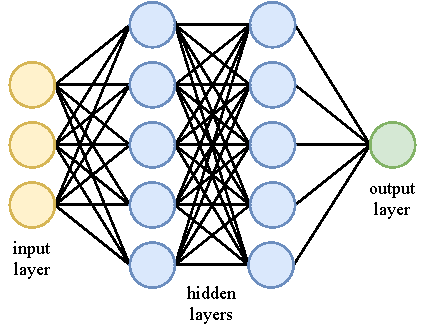
\includegraphics[width=0.6\textwidth]{diagrams/7-cvn/network.pdf}
    \caption[network short]
    {network long}
    \label{fig:network}
\end{figure}

\begin{equation} % MEAN-SQUARED ERROR LOSS EQUATION %
    E(\boldsymbol{w})=
    \frac{1}{n}\displaystyle\sum_{i=1}^{n}(y_{i}-
    \hat{y}_{i}(\boldsymbol{w}))^{2}
\end{equation}

\begin{equation} % BINARY CROSS-ENTROPY EQUATION %
    E(\boldsymbol{w})=
    -\displaystyle\sum_{i=1}^{n}y_{i}\log\hat{y}_{i}(\boldsymbol{w})+
    (1-y_{i})\log[1-\hat{y}_{i}(\boldsymbol{w})]
\end{equation}

\begin{equation} % CATEGORICAL CROSS-ENTROPY EQUATION %
    E(\boldsymbol{w})=
    -\displaystyle\sum_{i=1}^{n}\displaystyle\sum_{m=0}^{M-1}y_{im}\log\hat{y}_{im}
    (\boldsymbol{w})+(1-y_{im})\log[1-\hat{y}_{im}(\boldsymbol{w})]
\end{equation}

\subsection{Convolutional neural networks} %%%%%%%%%%%%%%%%%%%%%%%%%%%%%%%%%%%%%%%%%%%%%%%%%%%%%%%
\label{sec:cvn_theory_conv} %%%%%%%%%%%%%%%%%%%%%%%%%%%%%%%%%%%%%%%%%%%%%%%%%%%%%%%%%%%%%%%%%%%%%%

EQUATION: Back propogation equations derivation and explanation

\begin{figure} % ACTIVATIONS DIAGRAM %
    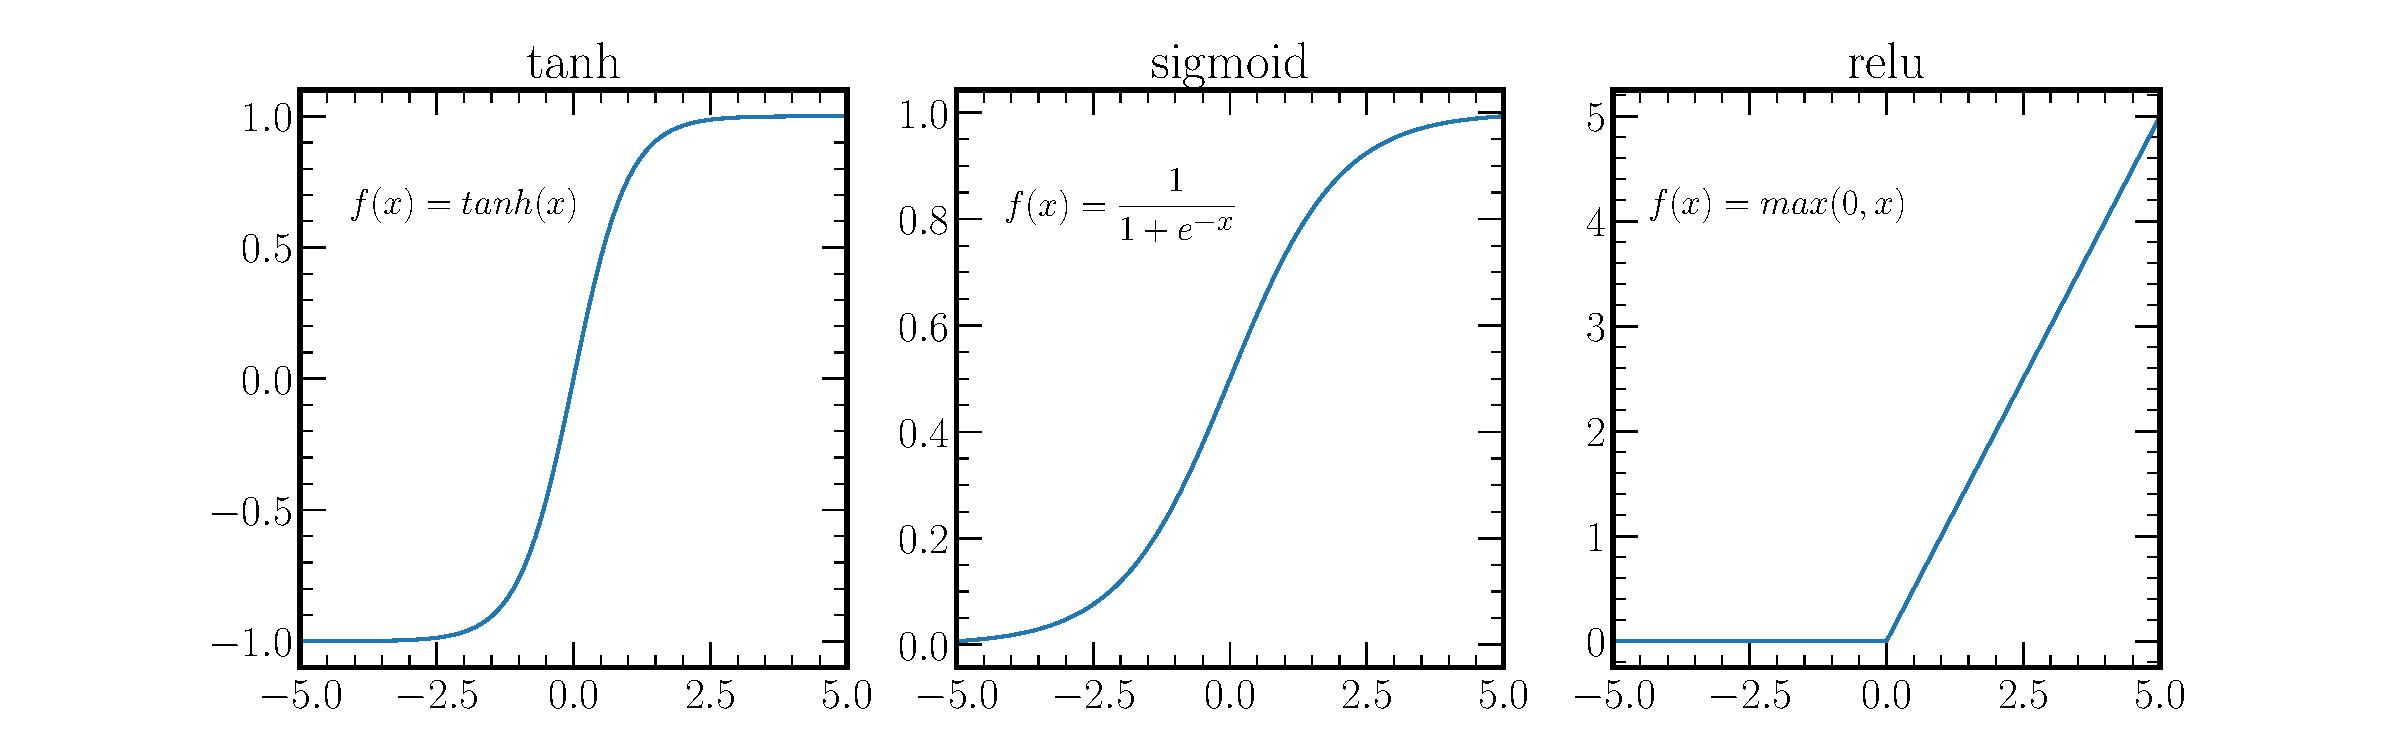
\includegraphics[width=\textwidth]{diagrams/7-cvn/activations.pdf}
    \caption[activations short]
    {activations long}
    \label{fig:activations}
\end{figure}

\begin{figure} % GRADIENT DESCENT DIAGRAM %
    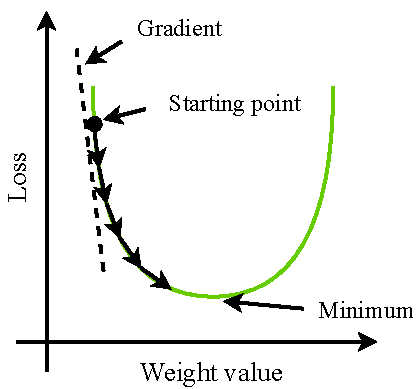
\includegraphics[width=0.5\textwidth]{diagrams/7-cvn/gradient_descent.pdf}
    \caption[gradient descent short]
    {gradient descent long}
    \label{fig:gradient_descent}
\end{figure}

\begin{figure} % CONV INPUTS DIAGRAM %
    \centering
    \begin{subfigure}[b]{0.3\textwidth}
        \centering
        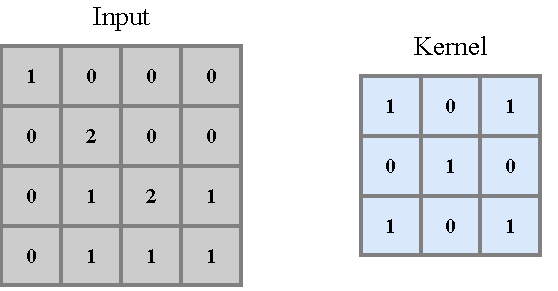
\includegraphics[width=\textwidth]{diagrams/7-cvn/conv_input.pdf}
        \caption{conv input long}
        \label{fig:conv_input}
    \end{subfigure}
    \hfill
    \begin{subfigure}[b]{0.3\textwidth}
        \centering
        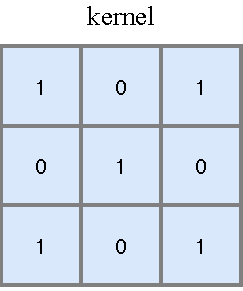
\includegraphics[width=\textwidth]{diagrams/7-cvn/conv_kernel.pdf}
        \caption{conv kernel long}
        \label{fig:conv_kernel}
    \end{subfigure}
    \caption{conv input and kernel}
    \label{fig:conv_input_kernel}
\end{figure}

TODO: combine the same and valid conv operations into the same diagram

\begin{figure} % CONV OPERATION DIAGRAM %
    \centering
    \begin{subfigure}[b]{0.71\textwidth}
        \centering
        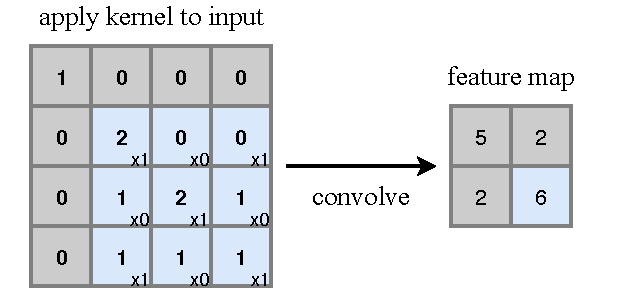
\includegraphics[width=\textwidth]{diagrams/7-cvn/conv_valid.pdf}
        \caption{conv valid long}
        \label{fig:conv_valid}
    \end{subfigure}
    \hfill
    \begin{subfigure}[b]{0.9\textwidth}
        \centering
        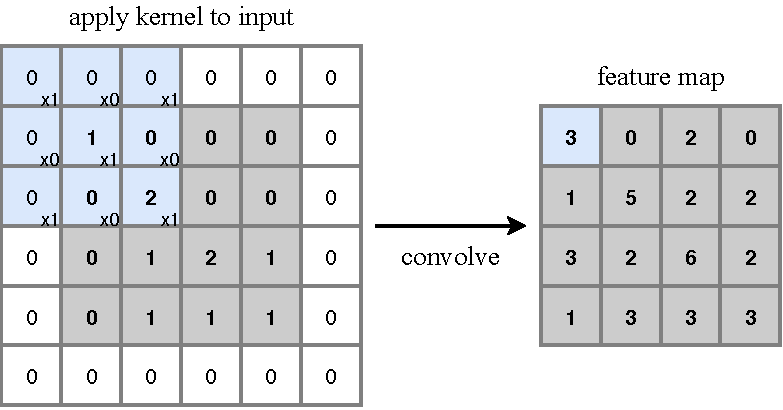
\includegraphics[width=\textwidth]{diagrams/7-cvn/conv_same.pdf}
        \caption{conv same long}
        \label{fig:conv_same}
    \end{subfigure}
    \caption{conv operations}
    \label{fig:conv_operations}
\end{figure}

\begin{figure} % POOLING DIAGRAM %
    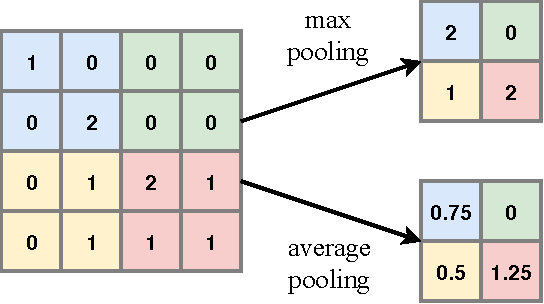
\includegraphics[width=0.6\textwidth]{diagrams/7-cvn/pooling.pdf}
    \caption[pooling short]
    {pooling long}
    \label{fig:pooling}
\end{figure}

\subsection{The evolution of convolutional networks} %%%%%%%%%%%%%%%%%%%%%%%%%%%%%%%%%%%%%%%%%%%%%
\label{sec:cvn_theory_architectures} %%%%%%%%%%%%%%%%%%%%%%%%%%%%%%%%%%%%%%%%%%%%%%%%%%%%%%%%%%%%%

- They truly caught the attention of the wider ML community in 2012 when A. Krizhevsky, I,
Sutskever and G. Hinton used a GPU to train AlexNet, lowering the error rate on the image
classification task ImageNet by 12%. 
- Such was the rapid pace of advance afterwards that the ResNet model achieved a 3.57\percent
error just three years later.

Original 'dropout' paper in Ref.~\cite{hinton2012}
Original Batch normalisation paper in Ref.~\cite{ioffe2015}
Bag of tricks in Ref.~\cite{he2019}
AlexNet paper in Ref.~\cite{krizhevsky2012}
VGG paper in Ref.~\cite{simonyan2014}
Original resnet paper in Ref.~\cite{he2016_original}
Improved resnet paper in Ref.~\cite{he2016_improved}
Inception-resnet paper in Ref.~\cite{szegedy2016}
Squeeze-and-excitation networks paper in Ref.~\cite{hu2018}
MobileNetV2 paper in Ref.~\cite{sandler2018}
EfficientNet paper in Ref.~\cite{tan2019}

EQUATION: Batch-normalisation equations

\begin{figure} % DROPOUT DIAGRAM %
    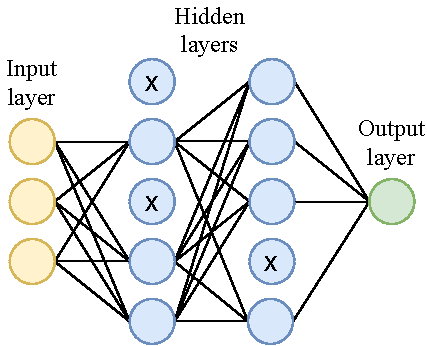
\includegraphics[width=0.6\textwidth]{diagrams/7-cvn/dropout.pdf}
    \caption[dropout short]
    {dropout long}
    \label{fig:dropout}
\end{figure}

\begin{figure} % EARLY STOPPING DIAGRAM %
    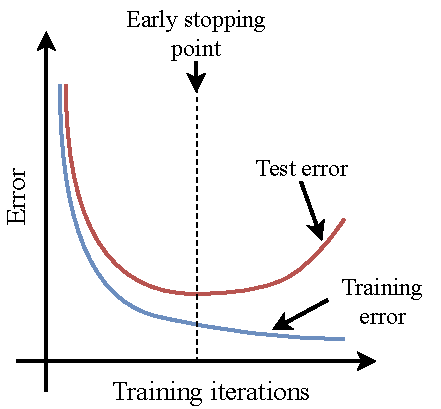
\includegraphics[width=0.5\textwidth]{diagrams/7-cvn/early_stopping.pdf}
    \caption[early stopping short]
    {early stopping long}
    \label{fig:early_stopping}
\end{figure}

\begin{figure} % SQUEEZE-EXITATION BLOCK DIAGRAM %
    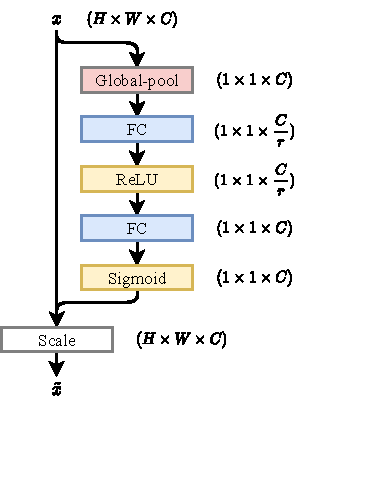
\includegraphics[width=0.5\textwidth]{diagrams/7-cvn/se.pdf}
    \caption[se short]
    {se long}
    \label{fig:se}
\end{figure}

\begin{figure} % RESNET BLOCK DIAGRAM %
    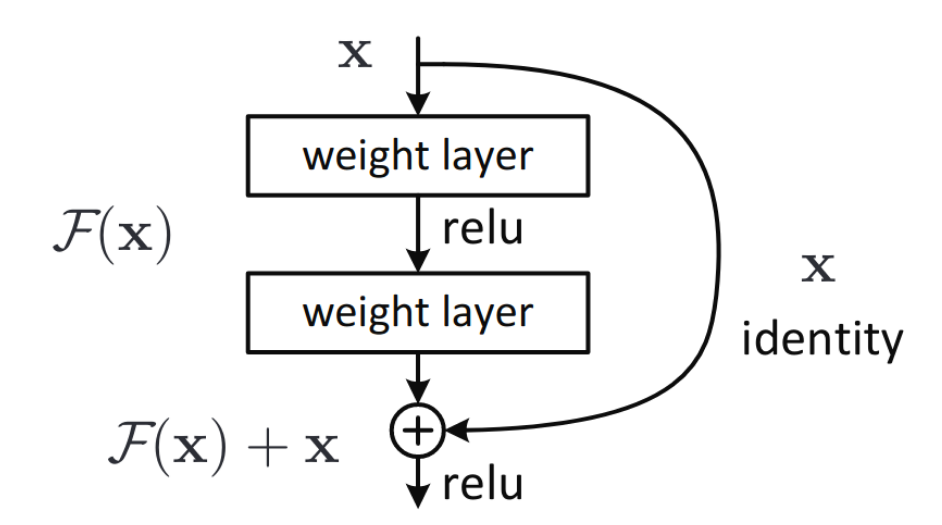
\includegraphics[width=0.6\textwidth]{diagrams/7-cvn/resnet_unit.png}
    \caption[resnet unit short]
    {resnet unit long}
    \label{fig:resnet_unit}
\end{figure}

\begin{figure} % INCEPTION BLOCK DIAGRAM %
    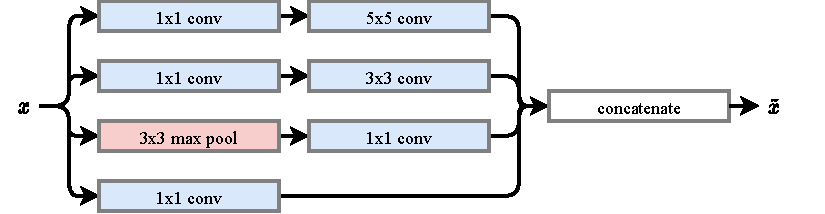
\includegraphics[width=0.8\textwidth]{diagrams/7-cvn/inception.pdf}
    \caption[inception short]
    {inception long}
    \label{fig:se}
\end{figure}

\section{A baseline implementation for CHIPS} %%%%%%%%%%%%%%%%%%%%%%%%%%%%%%%%%%%%%%%%%%%%%%%%%%%%
\label{sec:cvn_baseline} %%%%%%%%%%%%%%%%%%%%%%%%%%%%%%%%%%%%%%%%%%%%%%%%%%%%%%%%%%%%%%%%%%%%%%%%%

- Many high level libraries have now been formed, predominantly led by Tensorflow (from google)
and pyTorch (from facebook) making it easier to quickly code and implemented DNNs.

- Primary goal is to classify the neutrino flavour nuel CC, numu CC or NC
- Secondary goal is to then classify the individual interaction mode (QEL, RES, DIS etc...) these
will have different energy resolutions and systematic uncertainties, so seperation can provide
increased sensitivity.

\begin{figure} % NU ENERGIES DIAGRAM %
    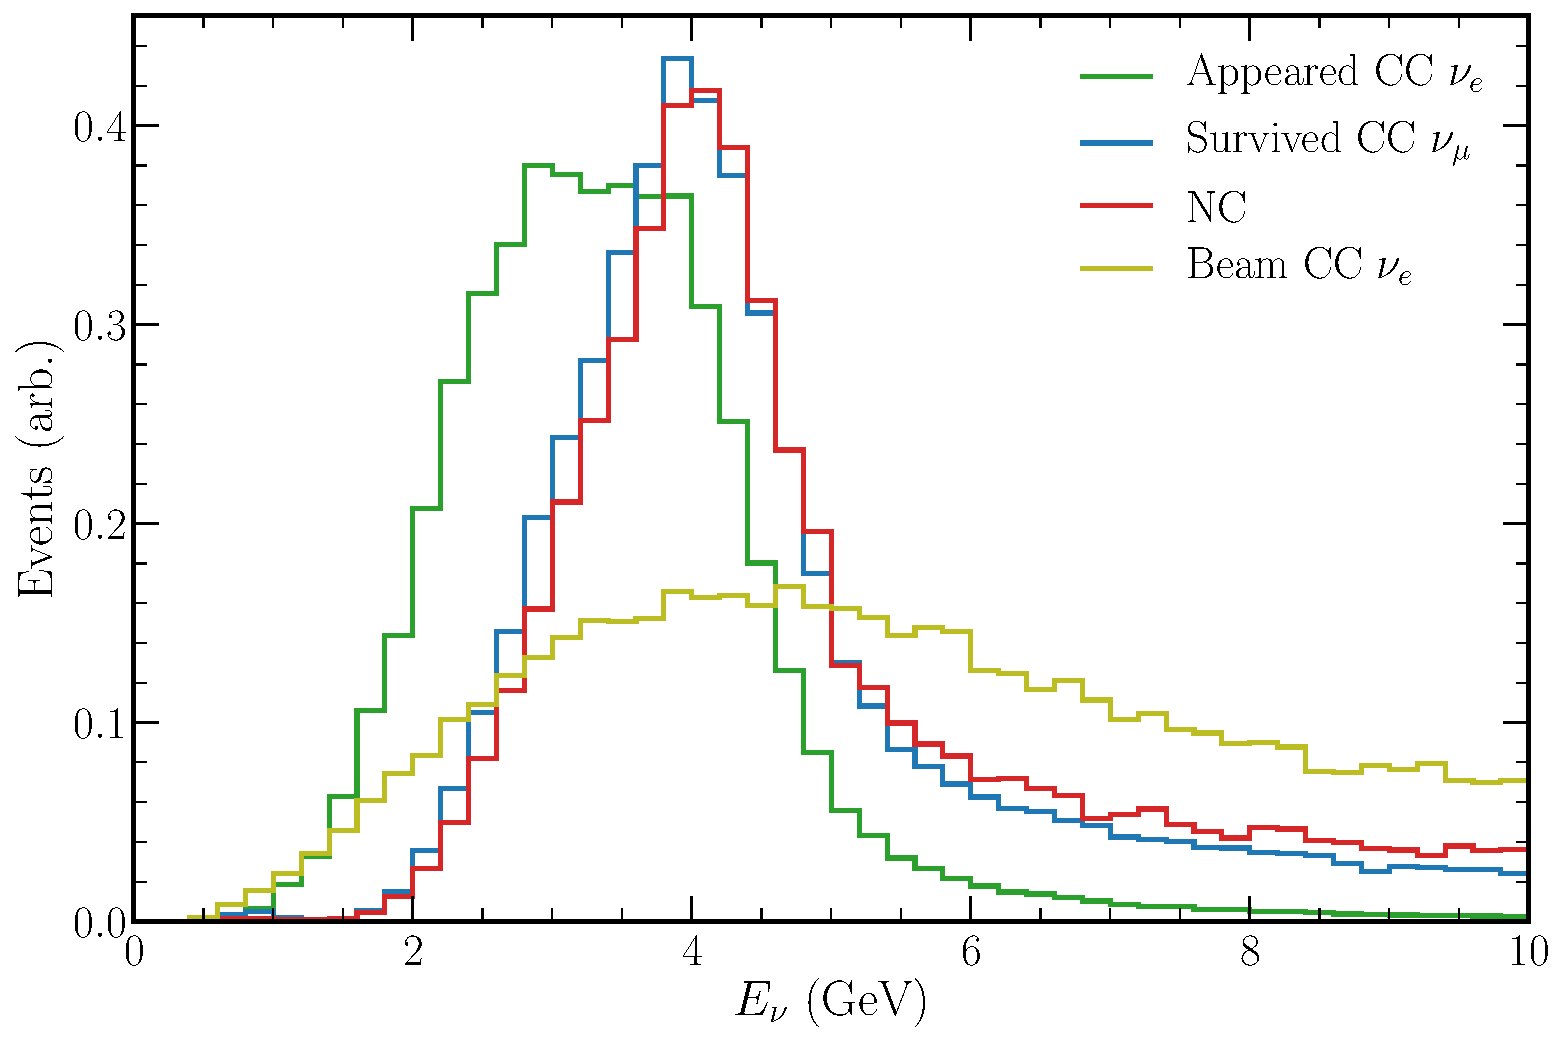
\includegraphics[width=0.6\textwidth]{diagrams/7-cvn/chipsnet/explore_nu_energies.pdf}
    \caption[explore nu energies short]
    {explore nu energies long}
    \label{fig:explore_nu_energies}
\end{figure}

\begin{figure} % OSC FLUXES DIAGRAM %
    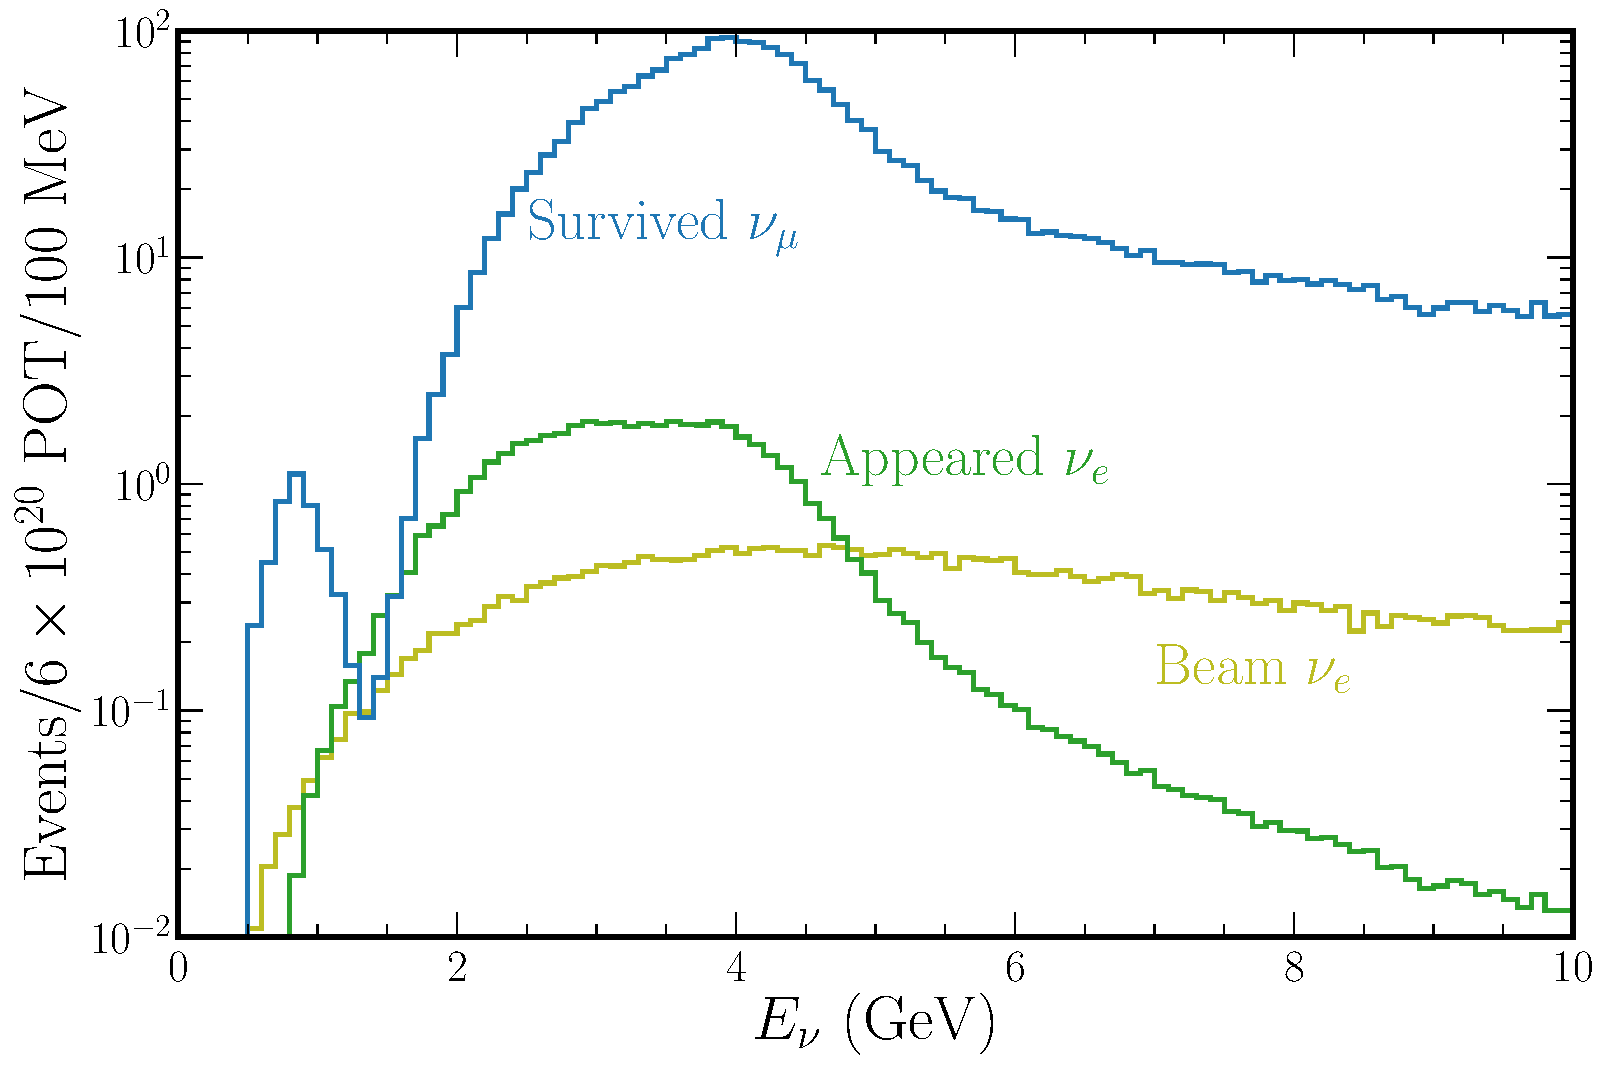
\includegraphics[width=0.6\textwidth]{diagrams/7-cvn/chipsnet/explore_osc_fluxes.pdf}
    \caption[explore osc fluxes short]
    {explore osc fluxes long}
    \label{fig:explore_osc_fluxes}
\end{figure}

\begin{figure} % SIMPLE CUTS DIAGRAM %
    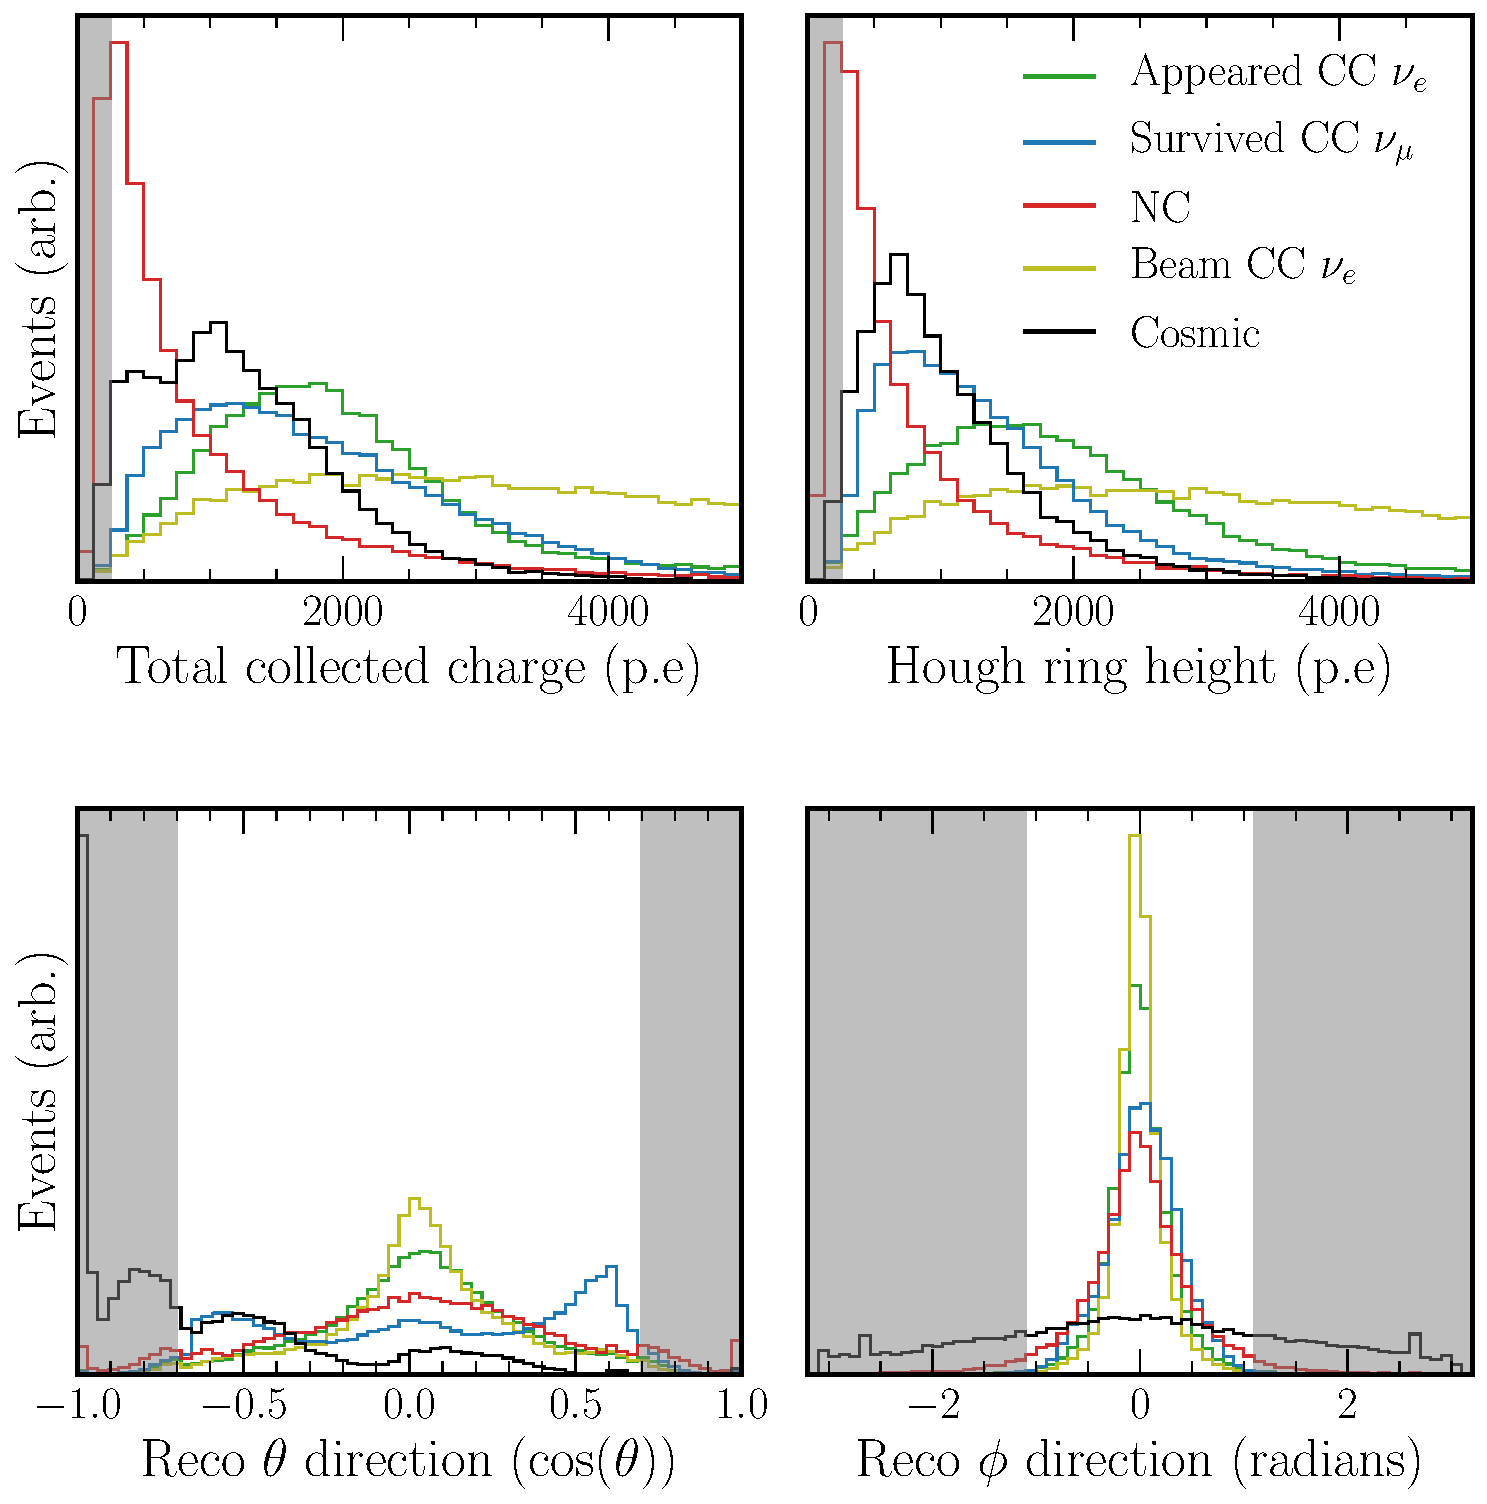
\includegraphics[width=0.8\textwidth]{diagrams/7-cvn/chipsnet/explore_simple_cuts.pdf}
    \caption[explore simple cuts short]
    {explore simple cuts long}
    \label{fig:explore_simple_cuts}
\end{figure}

\subsection{Software implementation} %%%%%%%%%%%%%%%%%%%%%%%%%%%%%%%%%%%%%%%%%%%%%%%%%%%%%%%%%%%%%
\label{sec:cvn_baseline_soft} %%%%%%%%%%%%%%%%%%%%%%%%%%%%%%%%%%%%%%%%%%%%%%%%%%%%%%%%%%%%%%%%%%%%

- Early stopping
- Model (dropout, batch norm, se, vgg etc...)

[0,25], outside range: 0.0010
    [0,120], outside range: 0.0015
    [0,3500], outside range: 0.0023

\begin{figure} % 8-BIT DIAGRAM %
    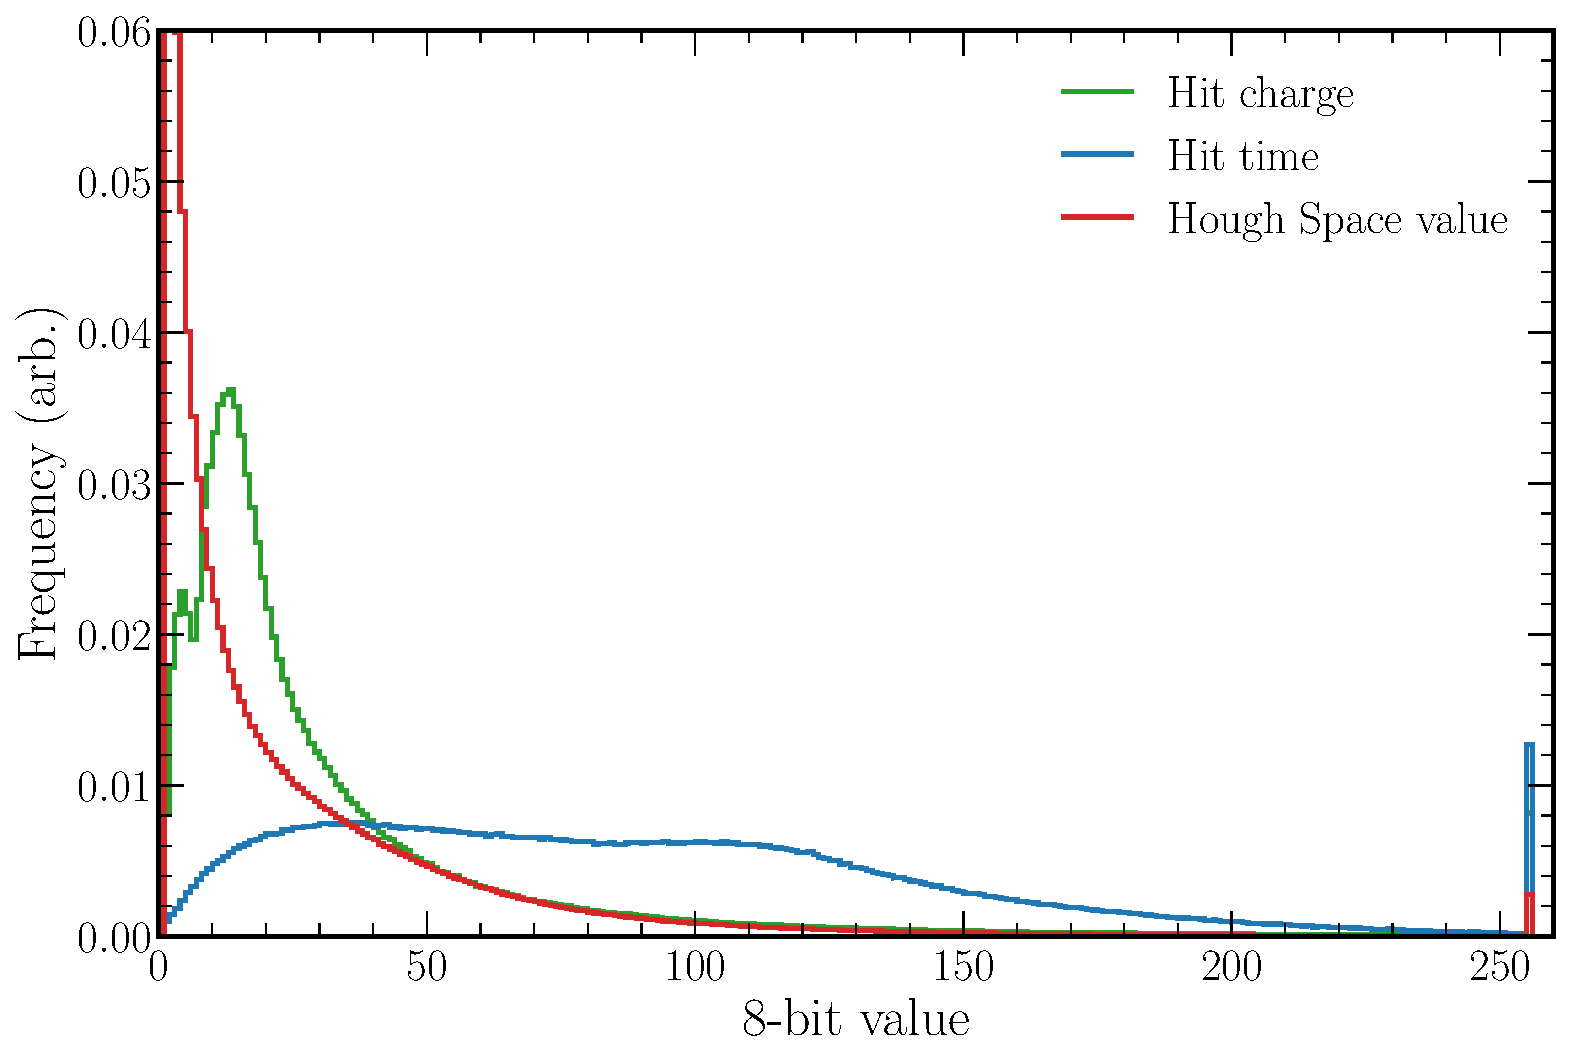
\includegraphics[width=0.6\textwidth]{diagrams/7-cvn/chipsnet/explore_8_bit_range.pdf}
    \caption[explore 8 bit range short]
    {explore 8 bit range long}
    \label{fig:explore_8_bit_range}
\end{figure}

\subsection{Network architecture} %%%%%%%%%%%%%%%%%%%%%%%%%%%%%%%%%%%%%%%%%%%%%%%%%%%%%%%%%%%%%%%%
\label{sec:cvn_baseline_architecture} %%%%%%%%%%%%%%%%%%%%%%%%%%%%%%%%%%%%%%%%%%%%%%%%%%%%%%%%%%%%

\begin{figure} % CHIPSNET DIAGRAM %
    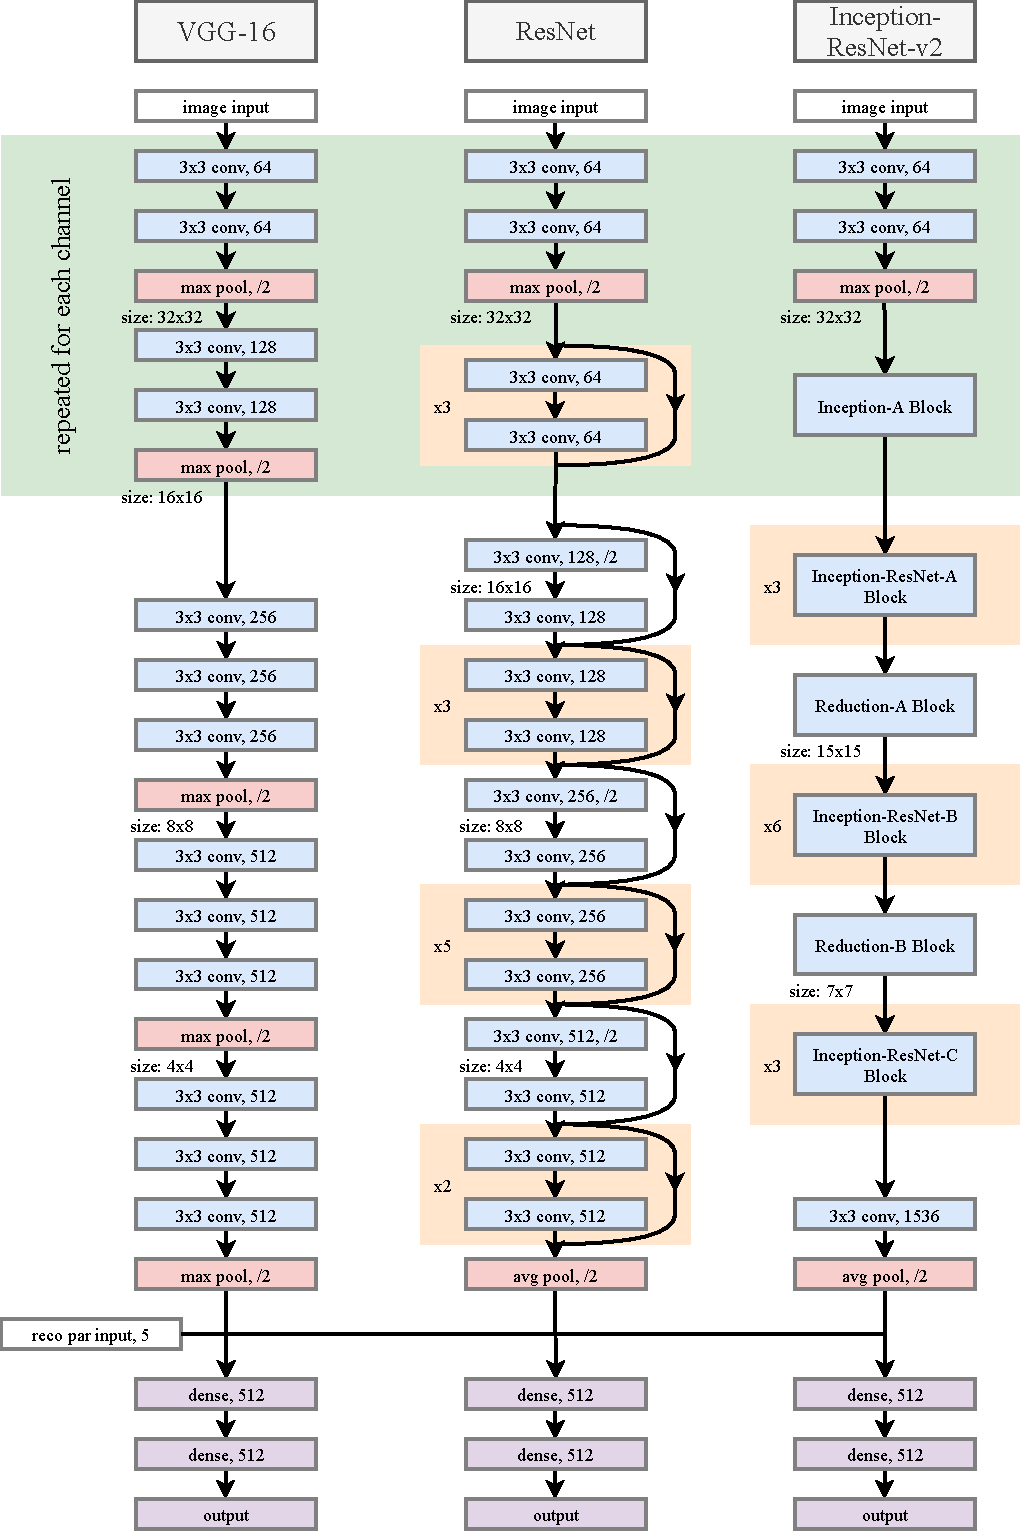
\includegraphics[width=\textwidth]{diagrams/7-cvn/chipsnet.pdf}
    \caption[chipsnet short]
    {chipsnet long}
    \label{fig:chipsnet}
\end{figure}

vgg: 17,225,296 (88ms)
inception: 16,893,216 (192ms)
resnet: 16,526,288 (112ms)
inception-resnet: 17,145,238 (209ms)

\begin{figure} % ARCHITECTURE NUEL EFF CURVES DIAGRAM %
    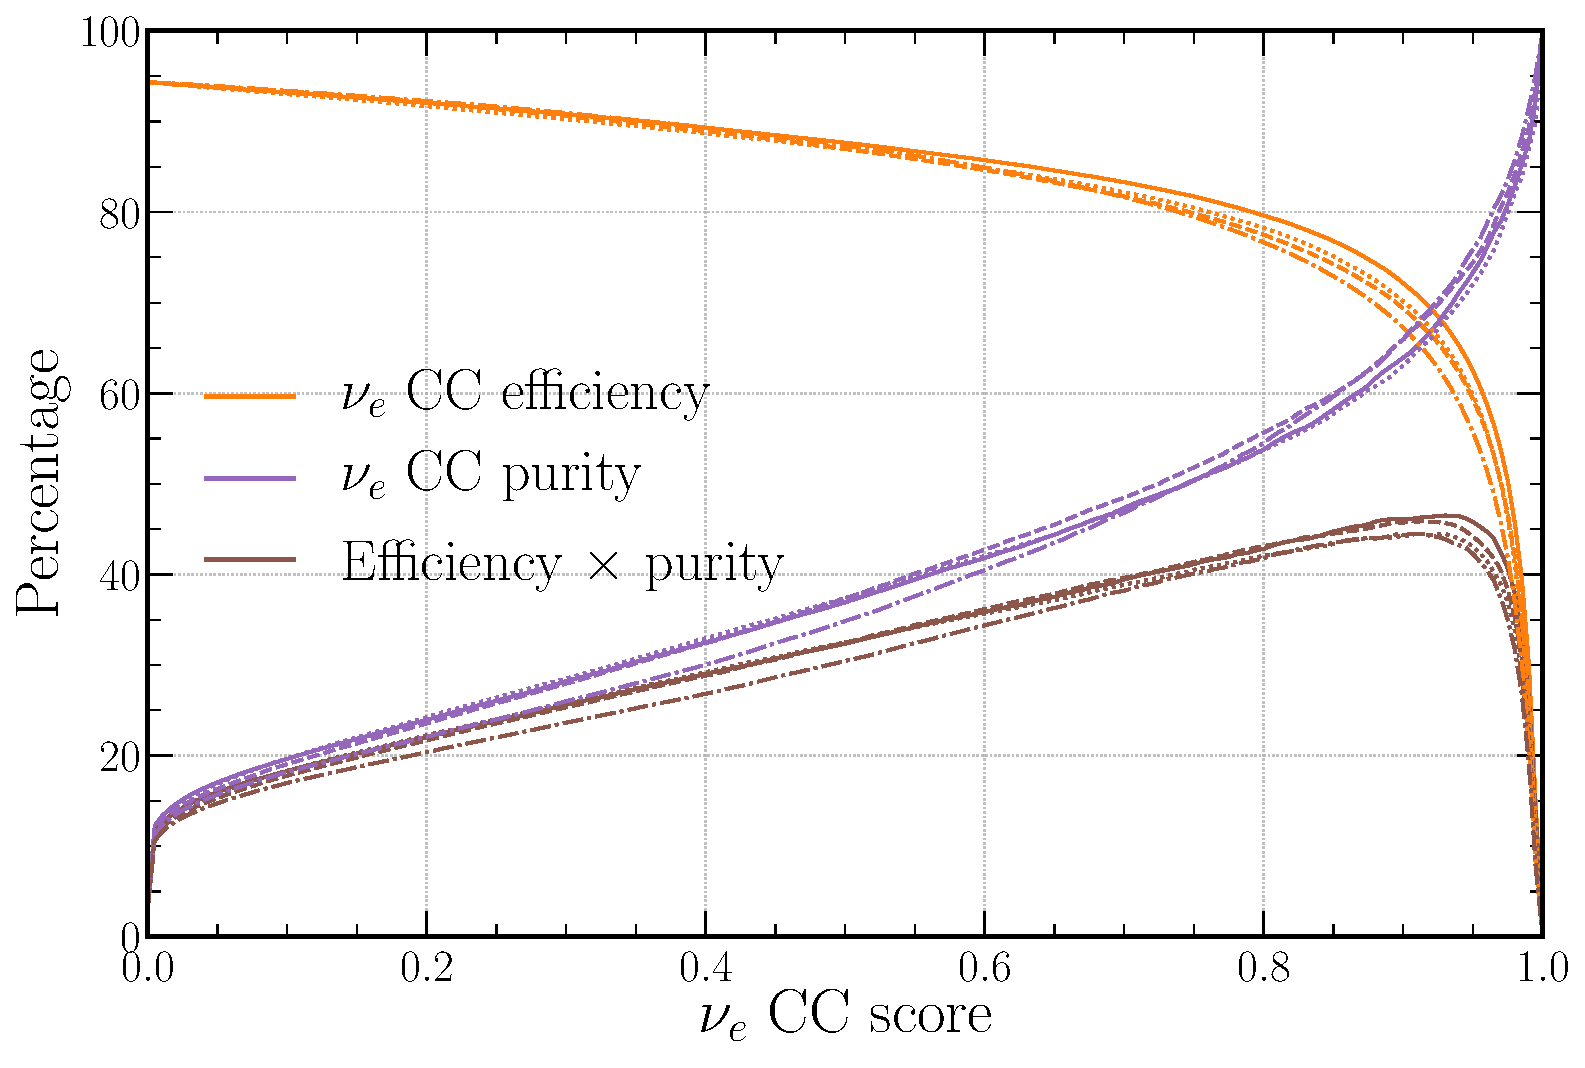
\includegraphics[width=0.6\textwidth]{diagrams/7-cvn/chipsnet/arch_nuel_eff_curves.pdf}
    \caption[arch nuel eff curves short]
    {vgg=solid, inception=dashed, resnet=dotted, inception-resnet=dot-dash}
    \label{fig:arch_nuel_eff_curves}
\end{figure}

\begin{figure} % ARCHITECTURE NUEL COMP CURVES DIAGRAM %
    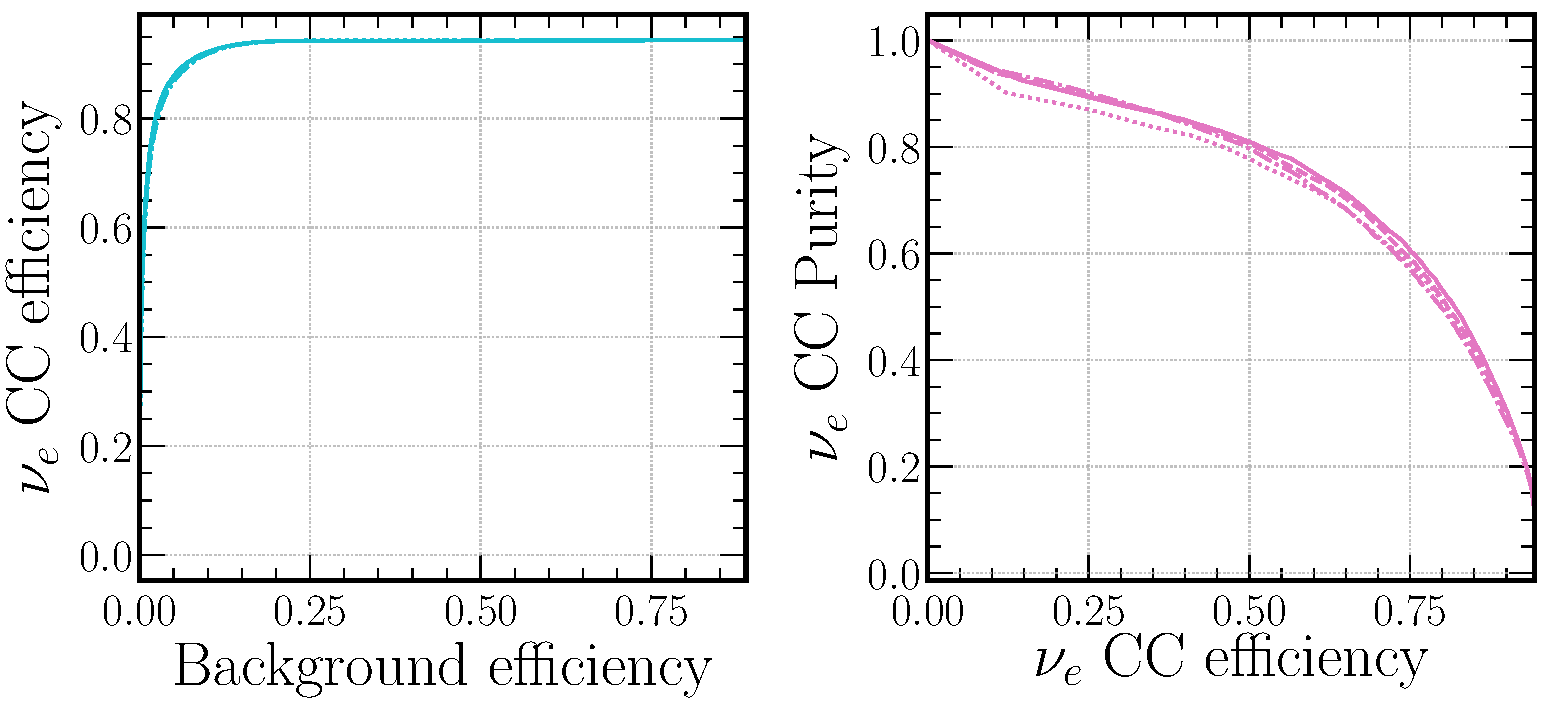
\includegraphics[width=0.8\textwidth]{diagrams/7-cvn/chipsnet/arch_nuel_comp_curves.pdf}
    \caption[arch nuel comp curves short]
    {vgg=solid, inception=dashed, resnet=dotted, inception-resnet=dot-dash}
    \label{fig:arch_nuel_comp_curves}
\end{figure}

- Nuel-> ROC-AUC: 0.82559, PRC-AUC: 0.71155, S-Eff: 0.87661, S-Pur: 0.36928
- FOM1-> 0.46510, 0.93000, 53.44422, 8.34671, 15.75487, 0.67485, 0.68920
- FOM2-> 13.44645, 0.98500, 31.21664, 1.57028, 3.81933, 0.39418, 0.85277

- Nuel-> ROC-AUC: 0.82519, PRC-AUC: 0.70632, S-Eff: 0.86992, S-Pur: 0.37332
- FOM1-> 0.45910, 0.91500, 53.20954, 9.73154, 14.92970, 0.67188, 0.68331
- FOM2-> 13.47965, 0.98500, 28.04995, 1.43802, 2.89217, 0.35419, 0.86627

- Nuel-> ROC-AUC: 0.82444, PRC-AUC: 0.68789, S-Eff: 0.86926, S-Pur: 0.37417
- FOM1-> 0.44511, 0.91000, 54.46409, 11.50537, 18.18029, 0.68772, 0.64723
- FOM2-> 12.22026, 0.98000, 32.56108, 2.77151, 4.32813, 0.41115, 0.82099

- Nuel-> ROC-AUC: 0.82444, PRC-AUC: 0.69946, S-Eff: 0.87369, S-Pur: 0.34882
- FOM1-> 0.44448, 0.90500, 52.61119, 10.90981, 15.11323, 0.66433, 0.66906
- FOM2-> 13.48962, 0.98500, 23.98040, 0.96809, 2.19211, 0.30280, 0.88356

\begin{figure} % ARCHITECTURE NUMU EFF CURVES DIAGRAM %
    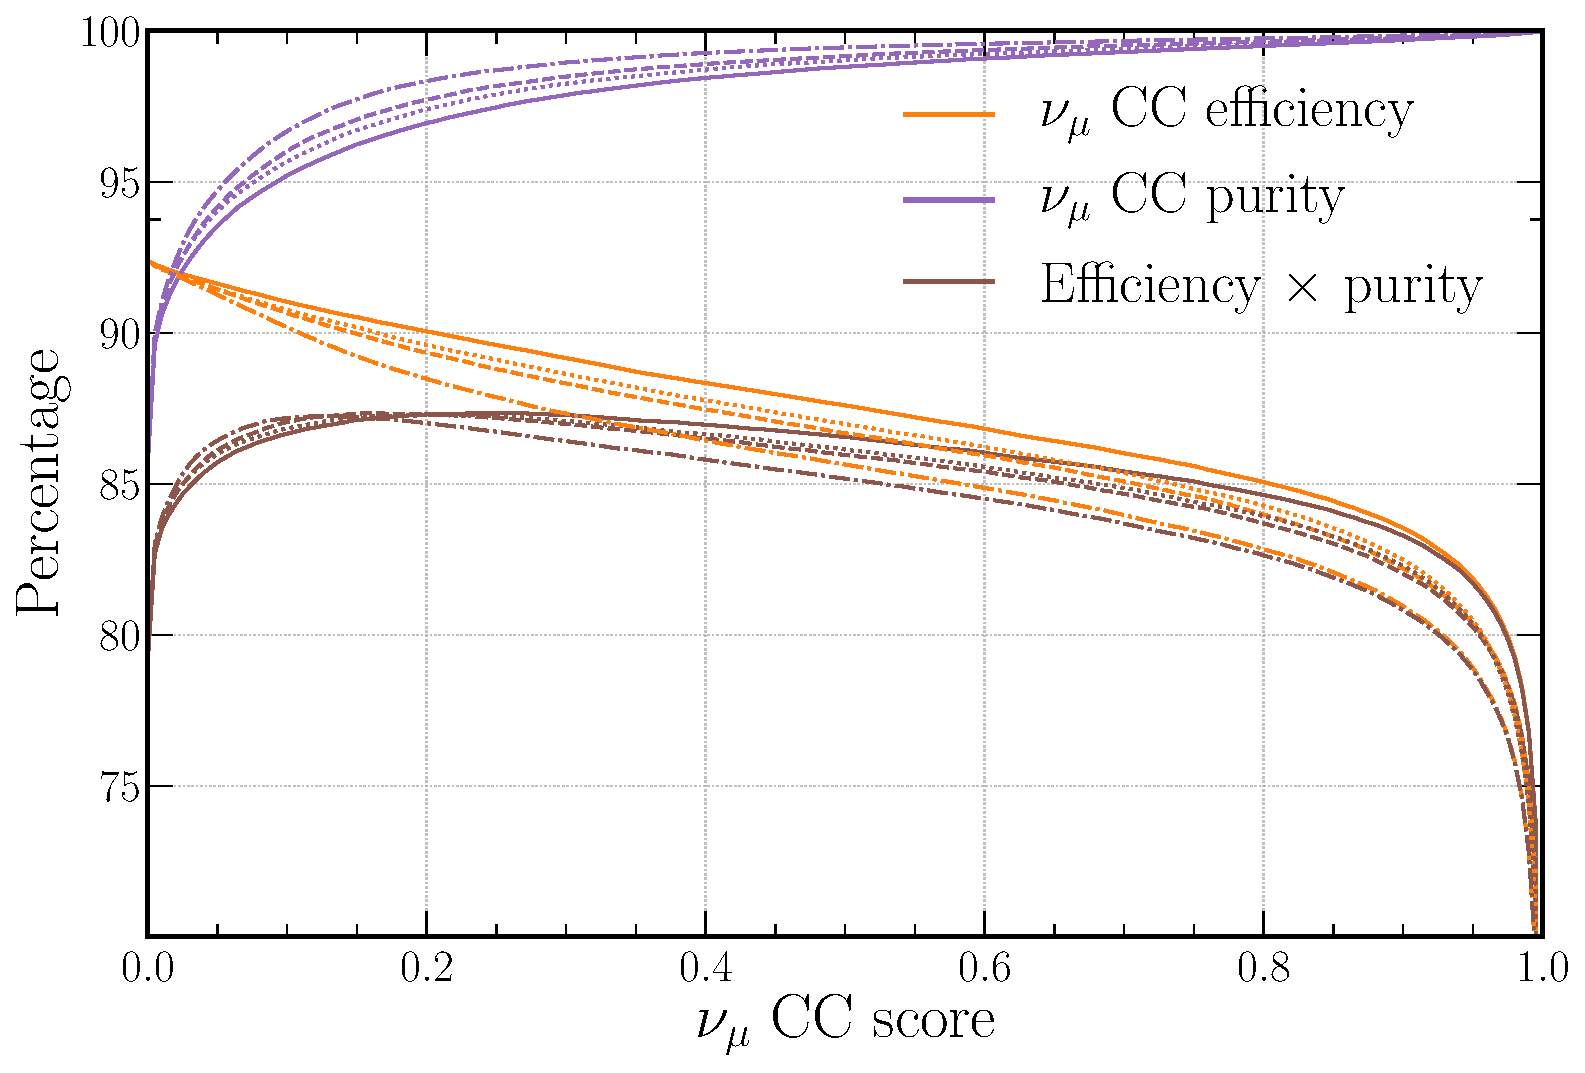
\includegraphics[width=0.6\textwidth]{diagrams/7-cvn/chipsnet/arch_numu_eff_curves.pdf}
    \caption[arch numu eff curves short]
    {vgg=solid, inception=dashed, resnet=dotted, inception-resnet=dot-dash}
    \label{fig:arch_numu_eff_curves}
\end{figure}

\begin{figure} % ARCHITECTURE NUMU COMP CURVES DIAGRAM %
    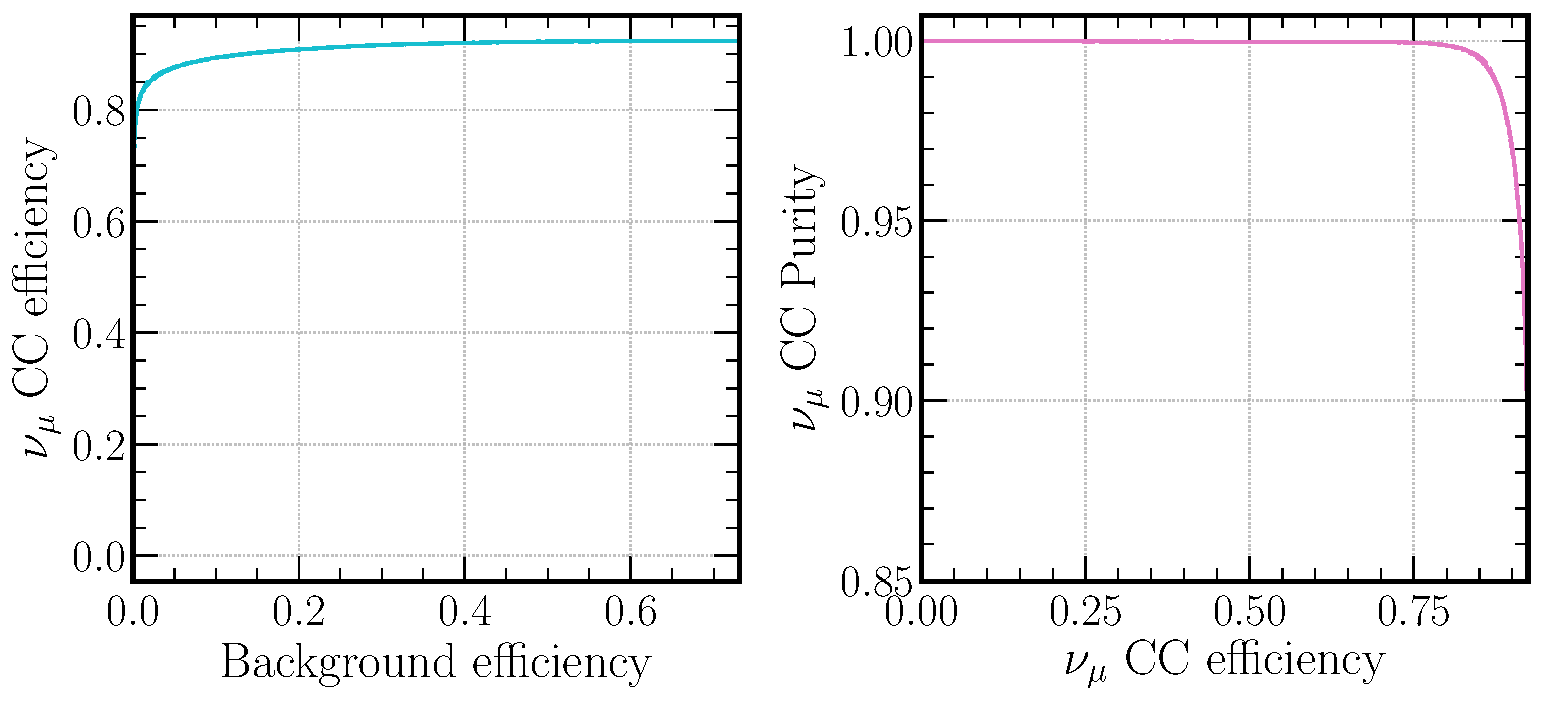
\includegraphics[width=0.8\textwidth]{diagrams/7-cvn/chipsnet/arch_numu_comp_curves.pdf}
    \caption[arch numu comp curves short]
    {vgg=solid, inception=dashed, resnet=dotted, inception-resnet=dot-dash}
    \label{fig:arch_numu_comp_curves}
\end{figure}

\subsection{Which training sample to use} %%%%%%%%%%%%%%%%%%%%%%%%%%%%%%%%%%%%%%%%%%%%%%%%%%%%%%%%
\label{sec:cvn_baseline_sample} %%%%%%%%%%%%%%%%%%%%%%%%%%%%%%%%%%%%%%%%%%%%%%%%%%%%%%%%%%%%%%%%%%

- See signal interactions peaked closely near score values of unity and the backgrounds lie close
to the zero score as expected.

\begin{figure} % FLUX TRAINING SAMPLE DIAGRAM %
    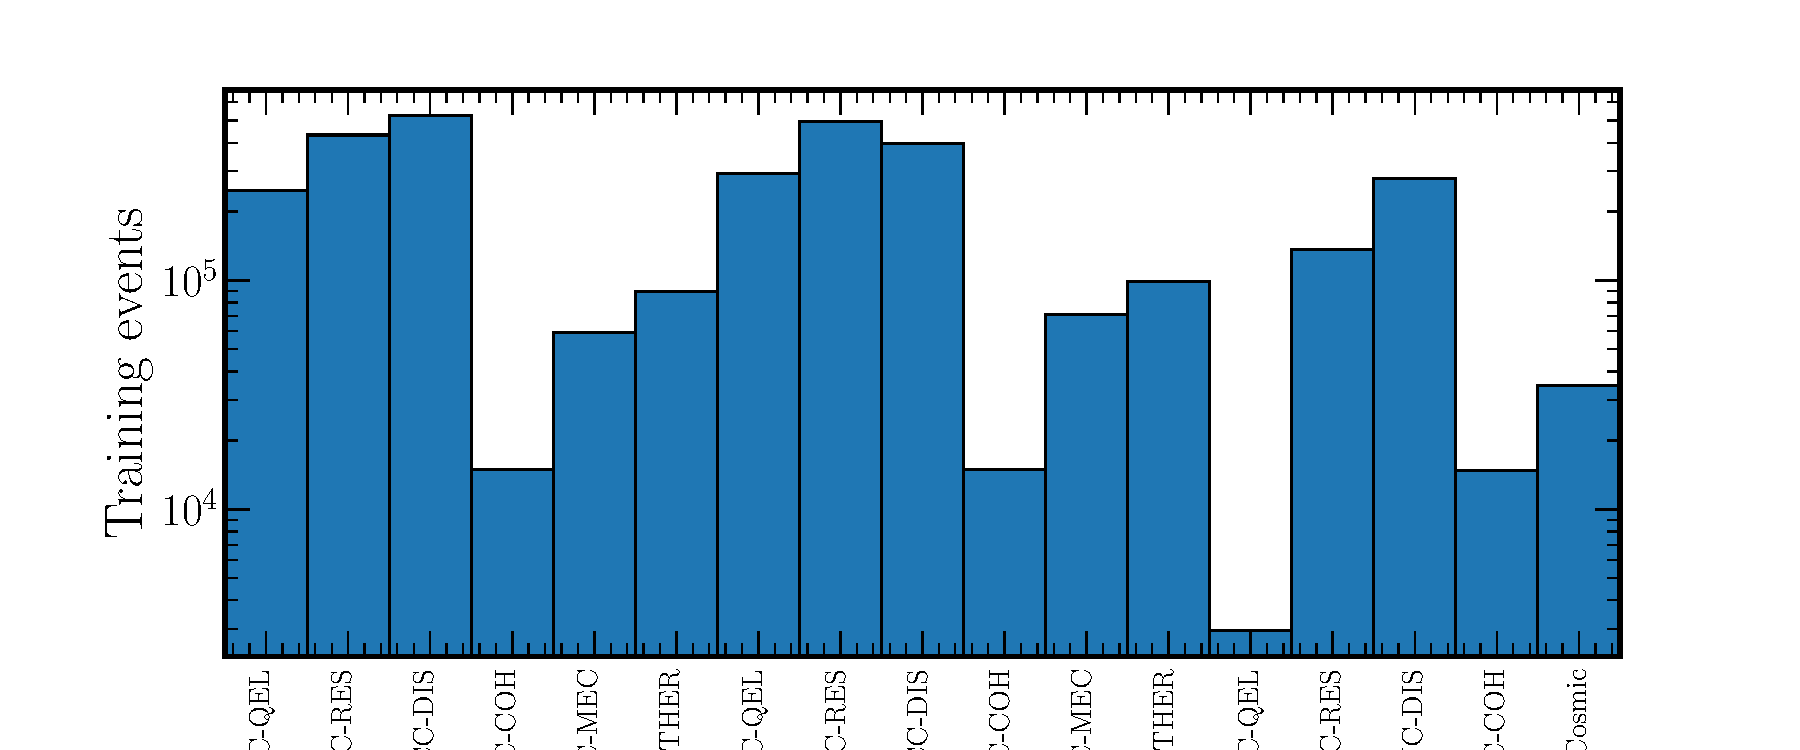
\includegraphics[width=0.6\textwidth]{diagrams/7-cvn/chipsnet/explore_flux_sample.pdf}
    \caption[explore flux sample short]
    {explore flux sample long}
    \label{fig:explore_flux_sample}
\end{figure}

\begin{figure} % UNIFORM TRAINING SAMPLE DIAGRAM %
    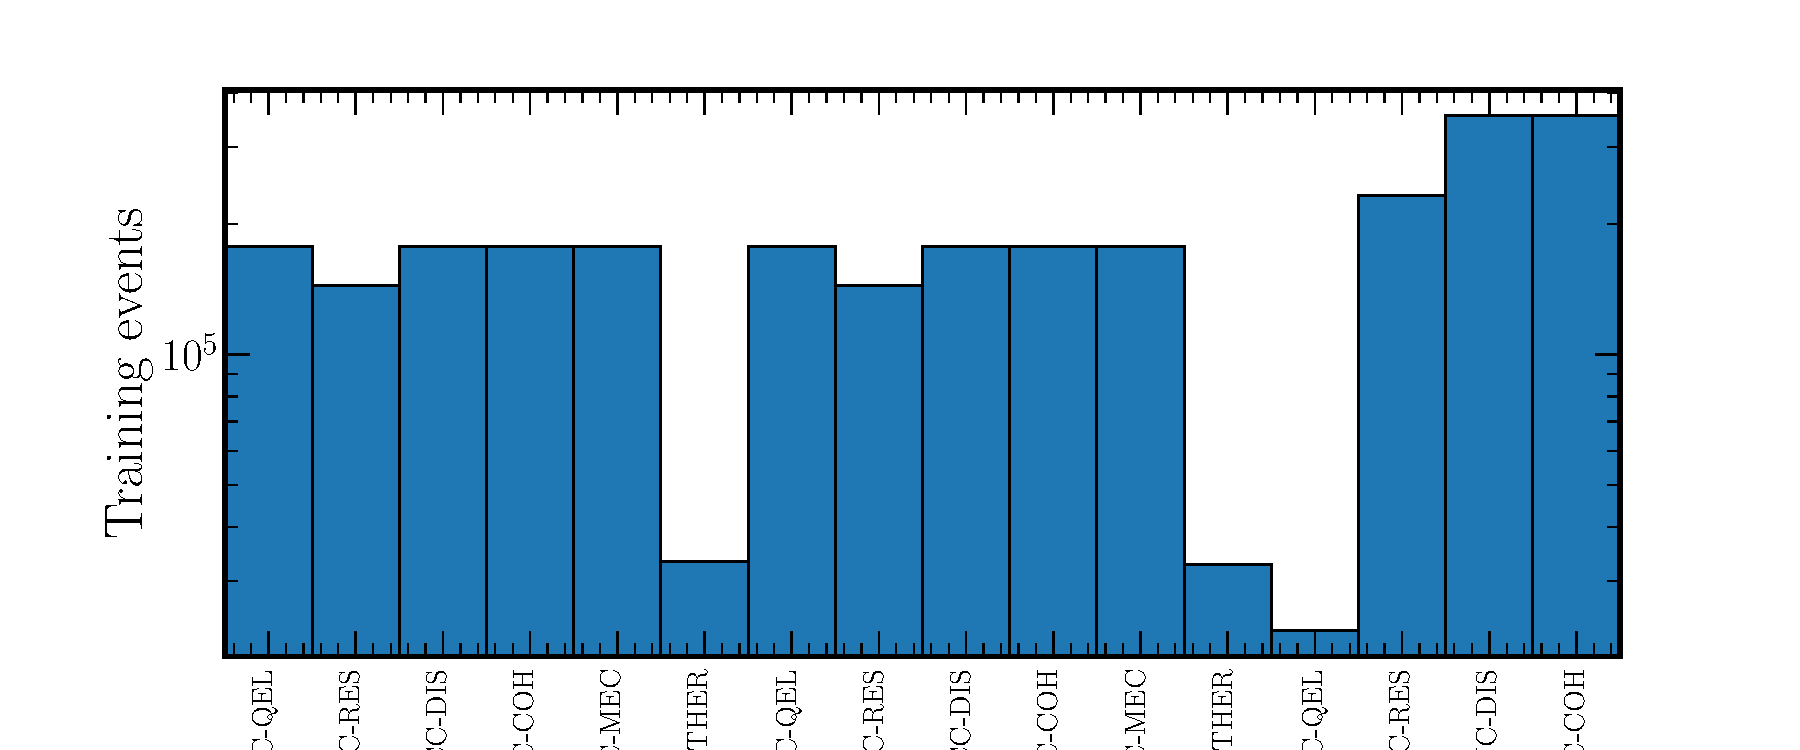
\includegraphics[width=0.6\textwidth]{diagrams/7-cvn/chipsnet/explore_uniform_sample.pdf}
    \caption[explore uniform sample short]
    {explore uniform sample long}
    \label{fig:explore_uniform_sample}
\end{figure}

\begin{figure} % BOTH TRAINING SAMPLE DIAGRAM %
    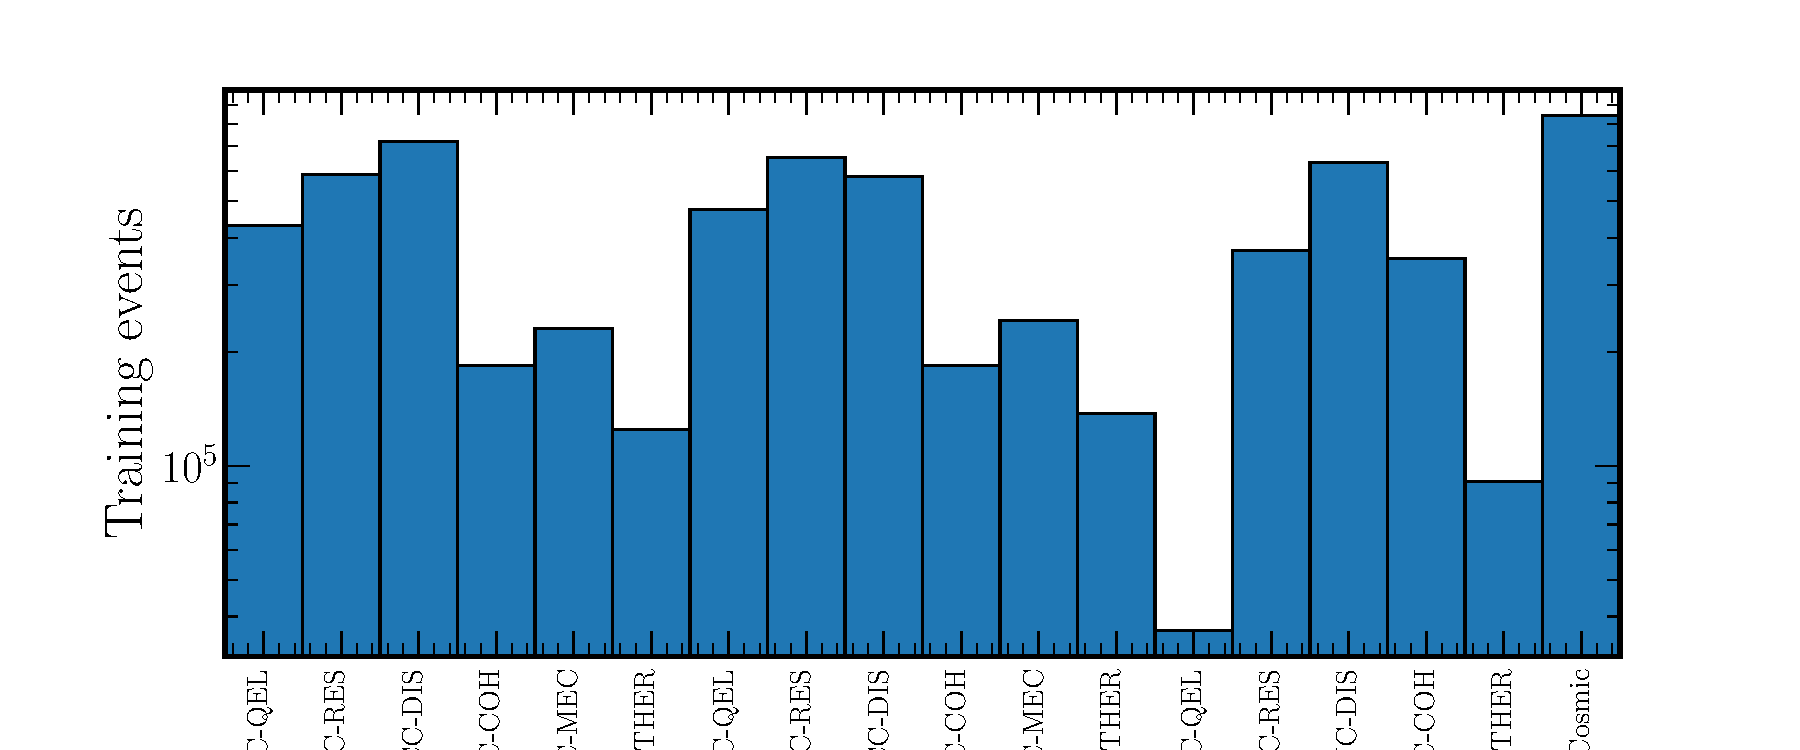
\includegraphics[width=0.6\textwidth]{diagrams/7-cvn/chipsnet/explore_both_sample.pdf}
    \caption[explore both sample short]
    {explore both sample long}
    \label{fig:explore_both_sample}
\end{figure}

\begin{figure} % SAMPLE FLUX OUTPUT DIAGRAM %
    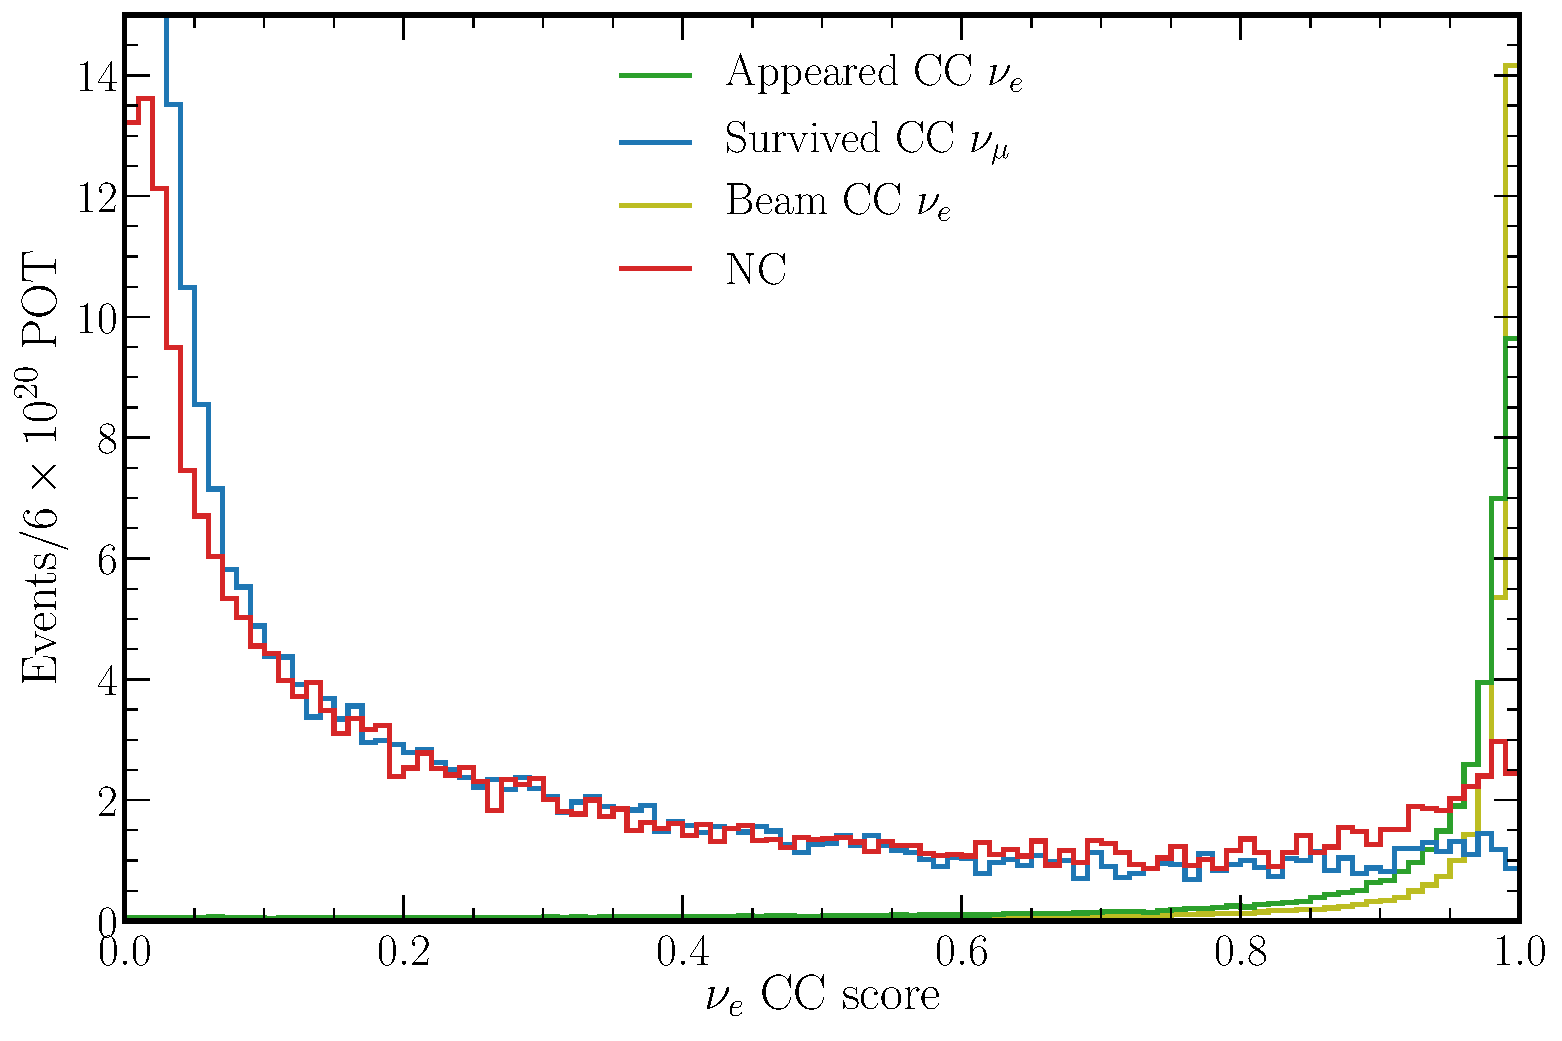
\includegraphics[width=0.6\textwidth]{diagrams/7-cvn/chipsnet/sample_flux_output_values.pdf}
    \caption[sample flux output values short]
    {sample flux output values long}
    \label{fig:sample_flux_output_values}
\end{figure}

\begin{figure} % SAMPLE UNIFORM OUTPUT DIAGRAM %
    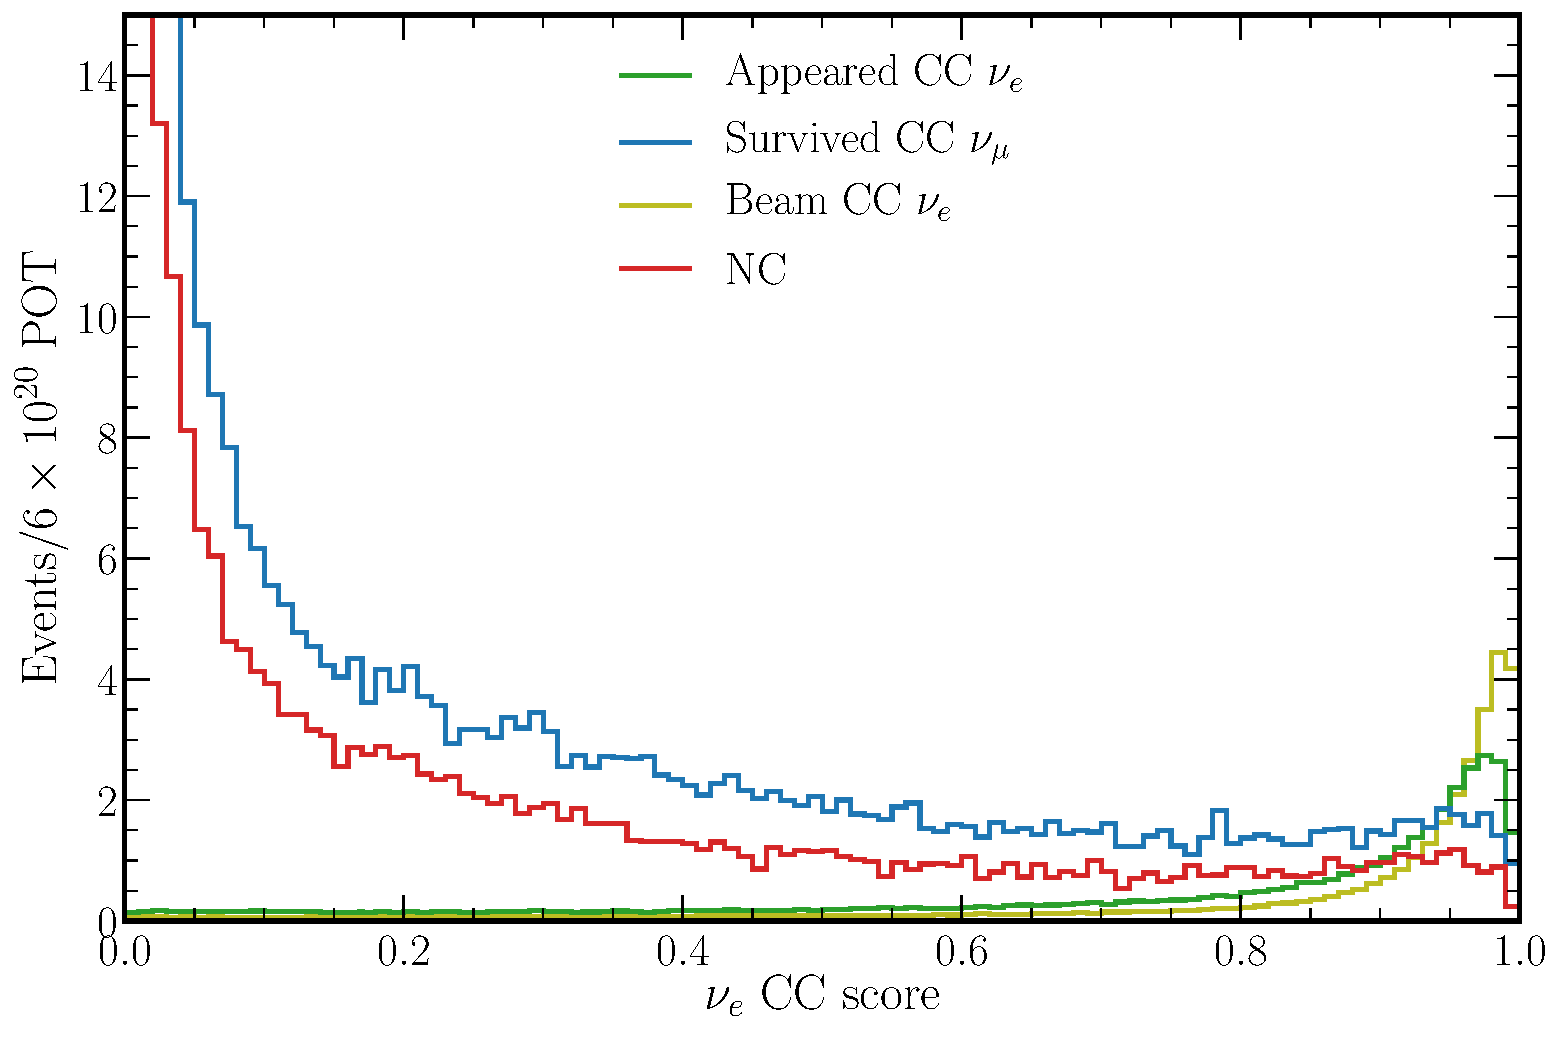
\includegraphics[width=0.6\textwidth]{diagrams/7-cvn/chipsnet/sample_uniform_output_values.pdf}
    \caption[sample uniform output values short]
    {sample uniform output values long}
    \label{fig:sample_uniform_output_values}
\end{figure}

\begin{figure} % SAMPLE BOTH OUTPUT DIAGRAM %
    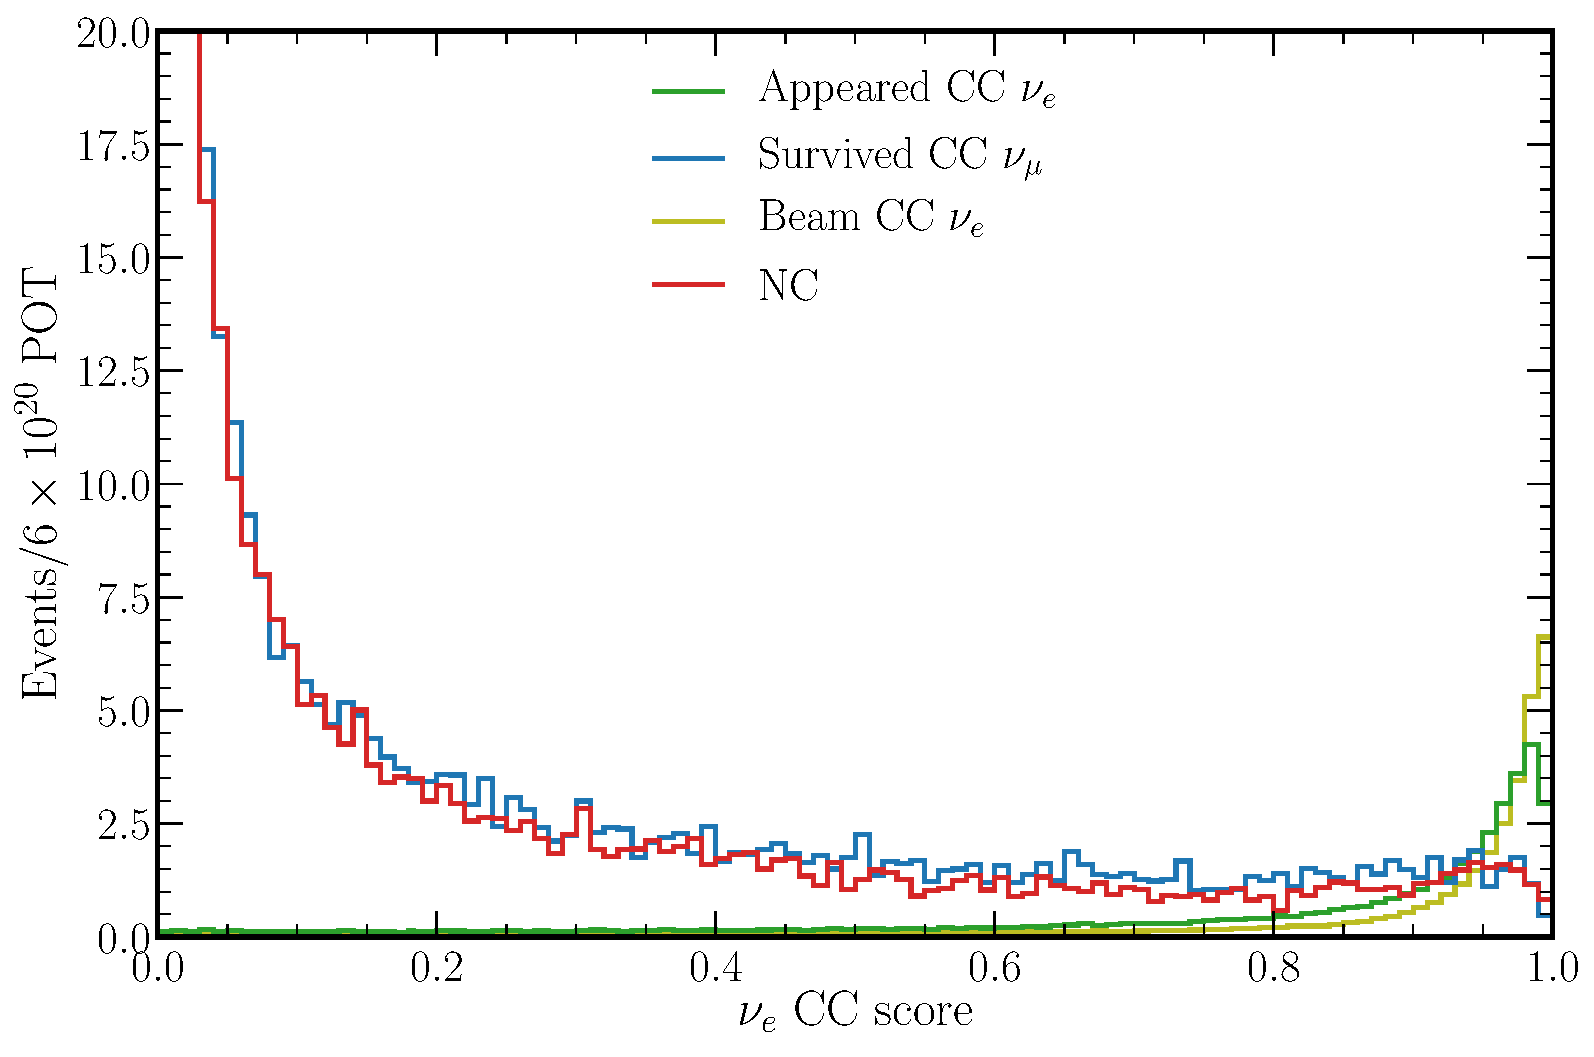
\includegraphics[width=0.6\textwidth]{diagrams/7-cvn/chipsnet/sample_both_output_values.pdf}
    \caption[sample both output values short]
    {sample both output values long}
    \label{fig:sample_both_output_values}
\end{figure}

\begin{figure} % SAMPLE NUEL EFF CURVES DIAGRAM %
    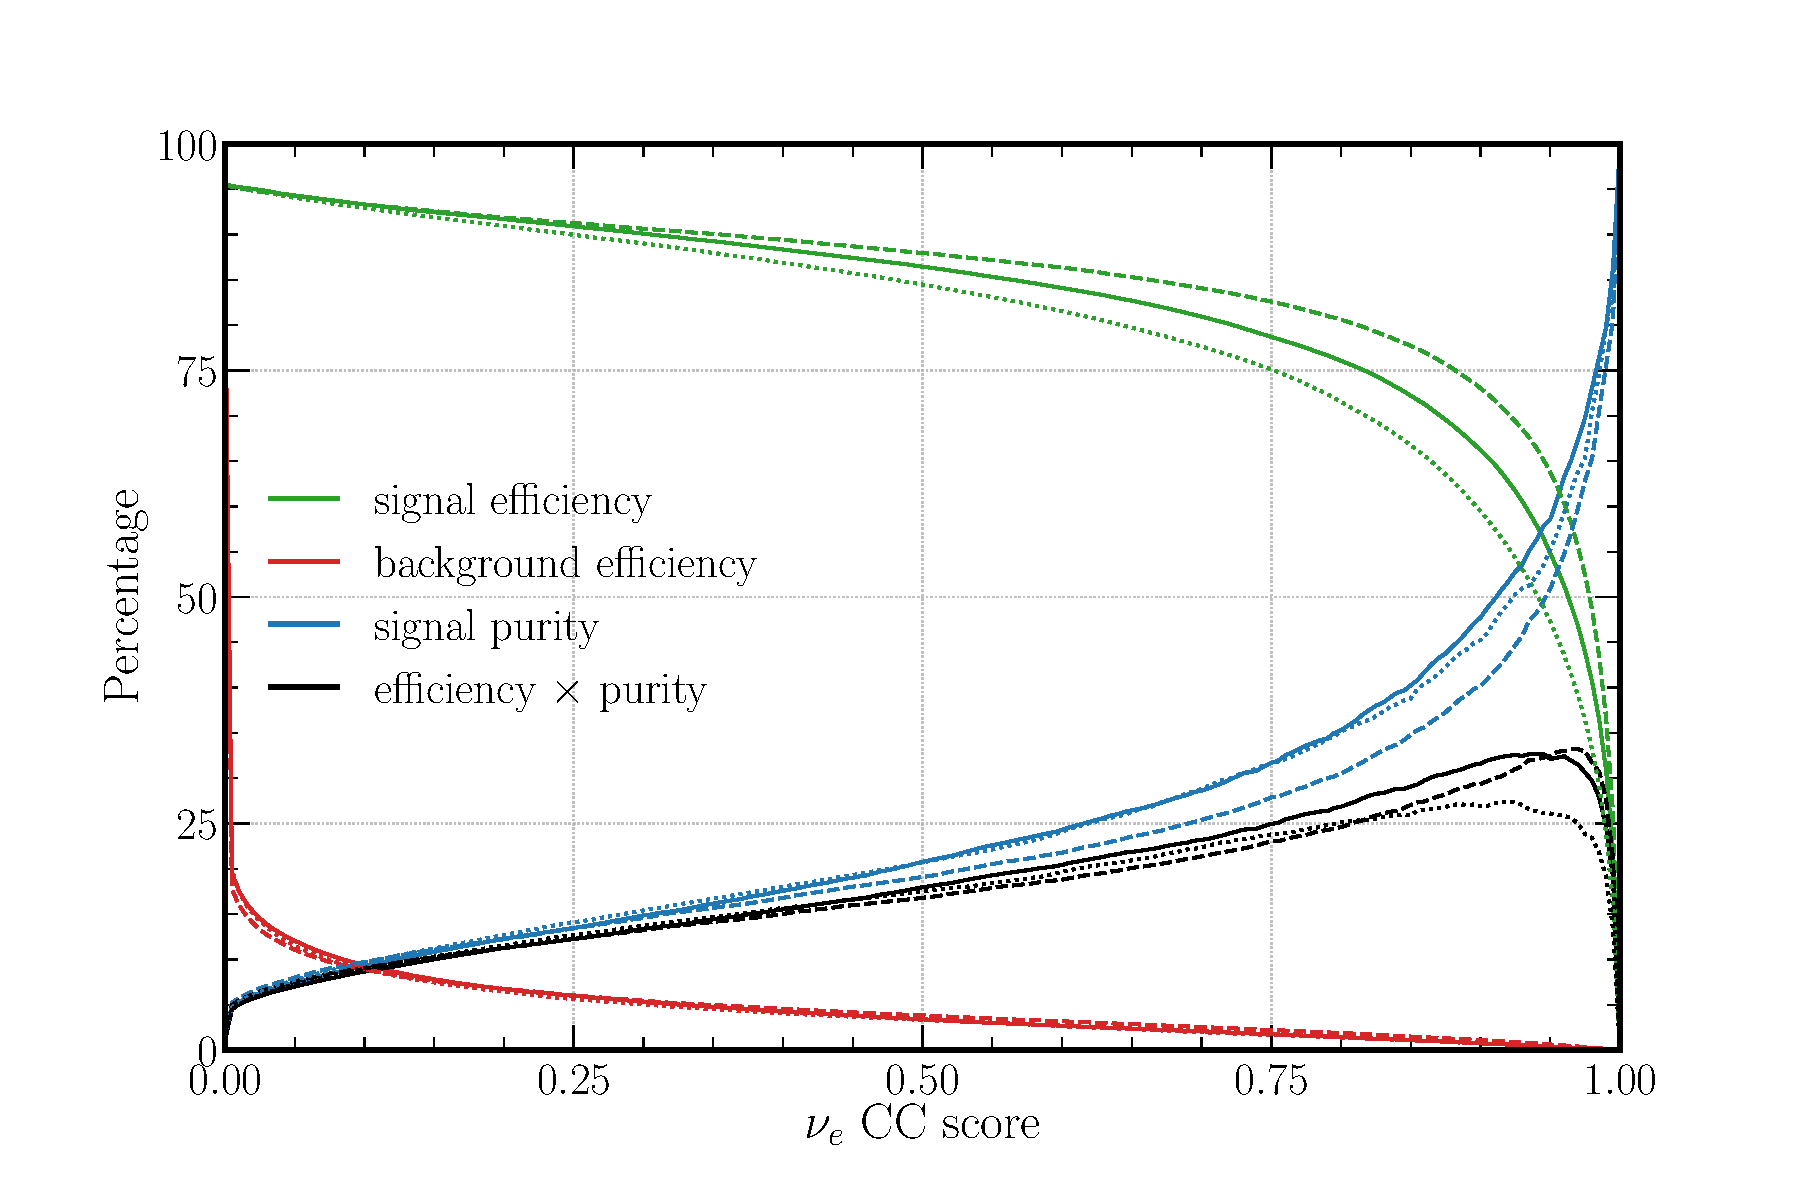
\includegraphics[width=0.6\textwidth]{diagrams/7-cvn/chipsnet/sample_nuel_eff_curves.pdf}
    \caption[sample nuel eff curves short]
    {both=solid, flux=dashed, uniform=dotted}
    \label{fig:sample_nuel_eff_curves}
\end{figure}

\begin{figure} % SAMPLE NUEL COMP CURVES DIAGRAM %
    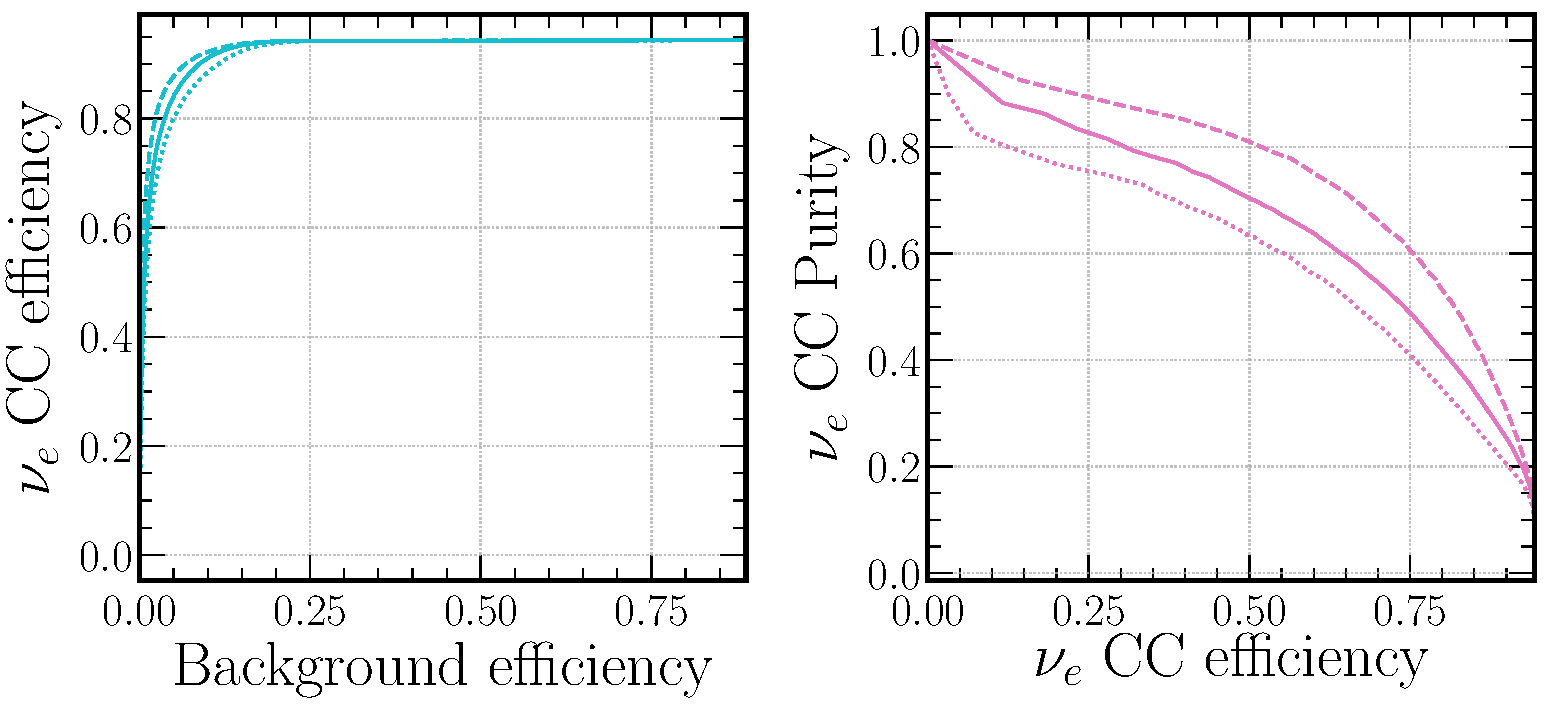
\includegraphics[width=0.8\textwidth]{diagrams/7-cvn/chipsnet/sample_nuel_comp_curves.pdf}
    \caption[sample nuel comp curves short]
    {both=solid, flux=dashed, uniform=dotted}
    \label{fig:sample_nuel_comp_curves}
\end{figure}

- Nuel-> ROC-AUC: 0.82559, PRC-AUC: 0.71155, S-Eff: 0.87661, S-Pur: 0.36928
- FOM1-> 0.46510, 0.93000, 53.44422, 8.34671, 15.75487, 0.67485, 0.68920
- FOM2-> 13.44645, 0.98500, 31.21664, 1.57028, 3.81933, 0.39418, 0.85277

- Nuel-> ROC-AUC: 0.81488, PRC-AUC: 0.56769, S-Eff: 0.79933, S-Pur: 0.34677
- FOM1-> 0.33905, 0.82500, 49.50120, 26.12079, 15.63656, 0.62506, 0.54243
- FOM2-> 8.44226, 0.92500, 36.01710, 11.59853, 6.60268, 0.45479, 0.66430

- Nuel-> ROC-AUC: 0.82063, PRC-AUC: 0.63426, S-Eff: 0.83421, S-Pur: 0.36814
- FOM1-> 0.38628, 0.84000, 52.60971, 19.59654, 18.26900, 0.66431, 0.58148
- FOM2-> 10.10769, 0.96000, 30.52599, 4.49055, 4.63030, 0.38545, 0.76995

\subsection{Which event representation to use} %%%%%%%%%%%%%%%%%%%%%%%%%%%%%%%%%%%%%%%%%%%%%%%%%%%
\label{sec:cvn_baseline_repr} %%%%%%%%%%%%%%%%%%%%%%%%%%%%%%%%%%%%%%%%%%%%%%%%%%%%%%%%%%%%%%%%%%%%

- Cern summer report in Ref.~\cite{theodore2016}
- New ideas with x+ x- mapping in Ref.~\cite{berns2020}
- Fraction of deposited charge in endcaps = 0.4769380479133997

- Approaches in the past for event classification using CNNs for water cherenkov detectors have
taken a few Approaches to generating the input image representation.
- Projecting onto a 2d surface "outside" the detector

\begin{figure} % NUEL EVENT DIAGRAM %
    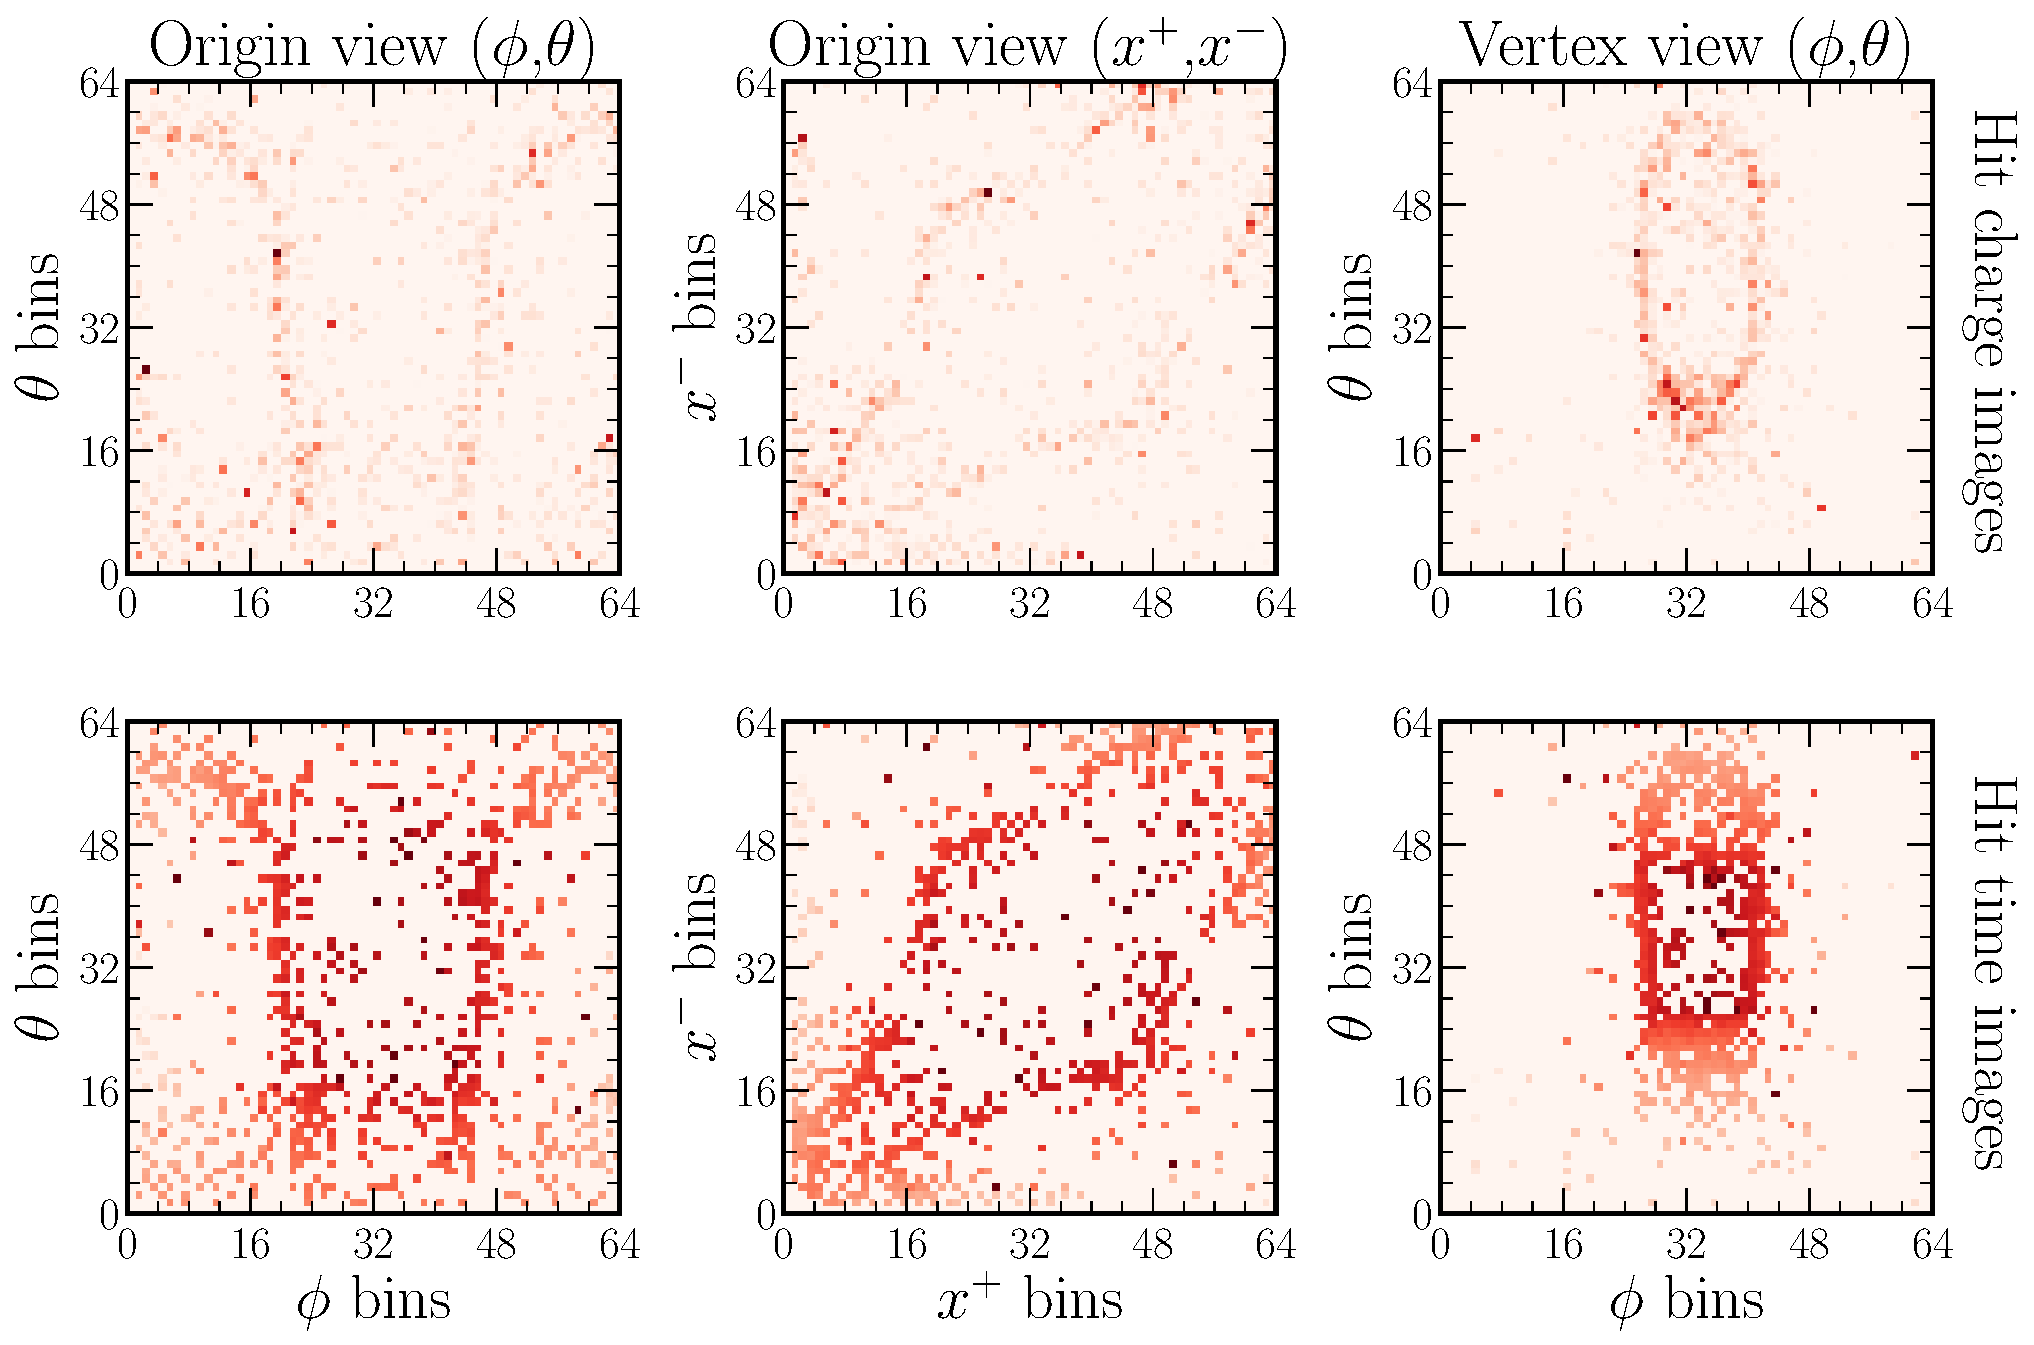
\includegraphics[width=0.8\textwidth]{diagrams/7-cvn/chipsnet/explore_nuel_ccres_event.pdf}
    \caption[explore nuel ccres event short]
    {3
        3307.41
        2777.48
            [  11 2212 2212  111 -999 -999 -999 -999 -999 -999 -999 -999 -999 -999
                -999 -999 -999 -999 -999 -999]
            [2777.48  1085.32   991.703  318.527 -999.    -999.    -999.    -999.
                -999.    -999.    -999.    -999.    -999.    -999.    -999.    -999.
                -999.    -999.    -999.    -999.   ]
        0}
    \label{fig:explore_nuel_ccres_event}
\end{figure}

\begin{figure} % NUMU EVENT DIAGRAM %
    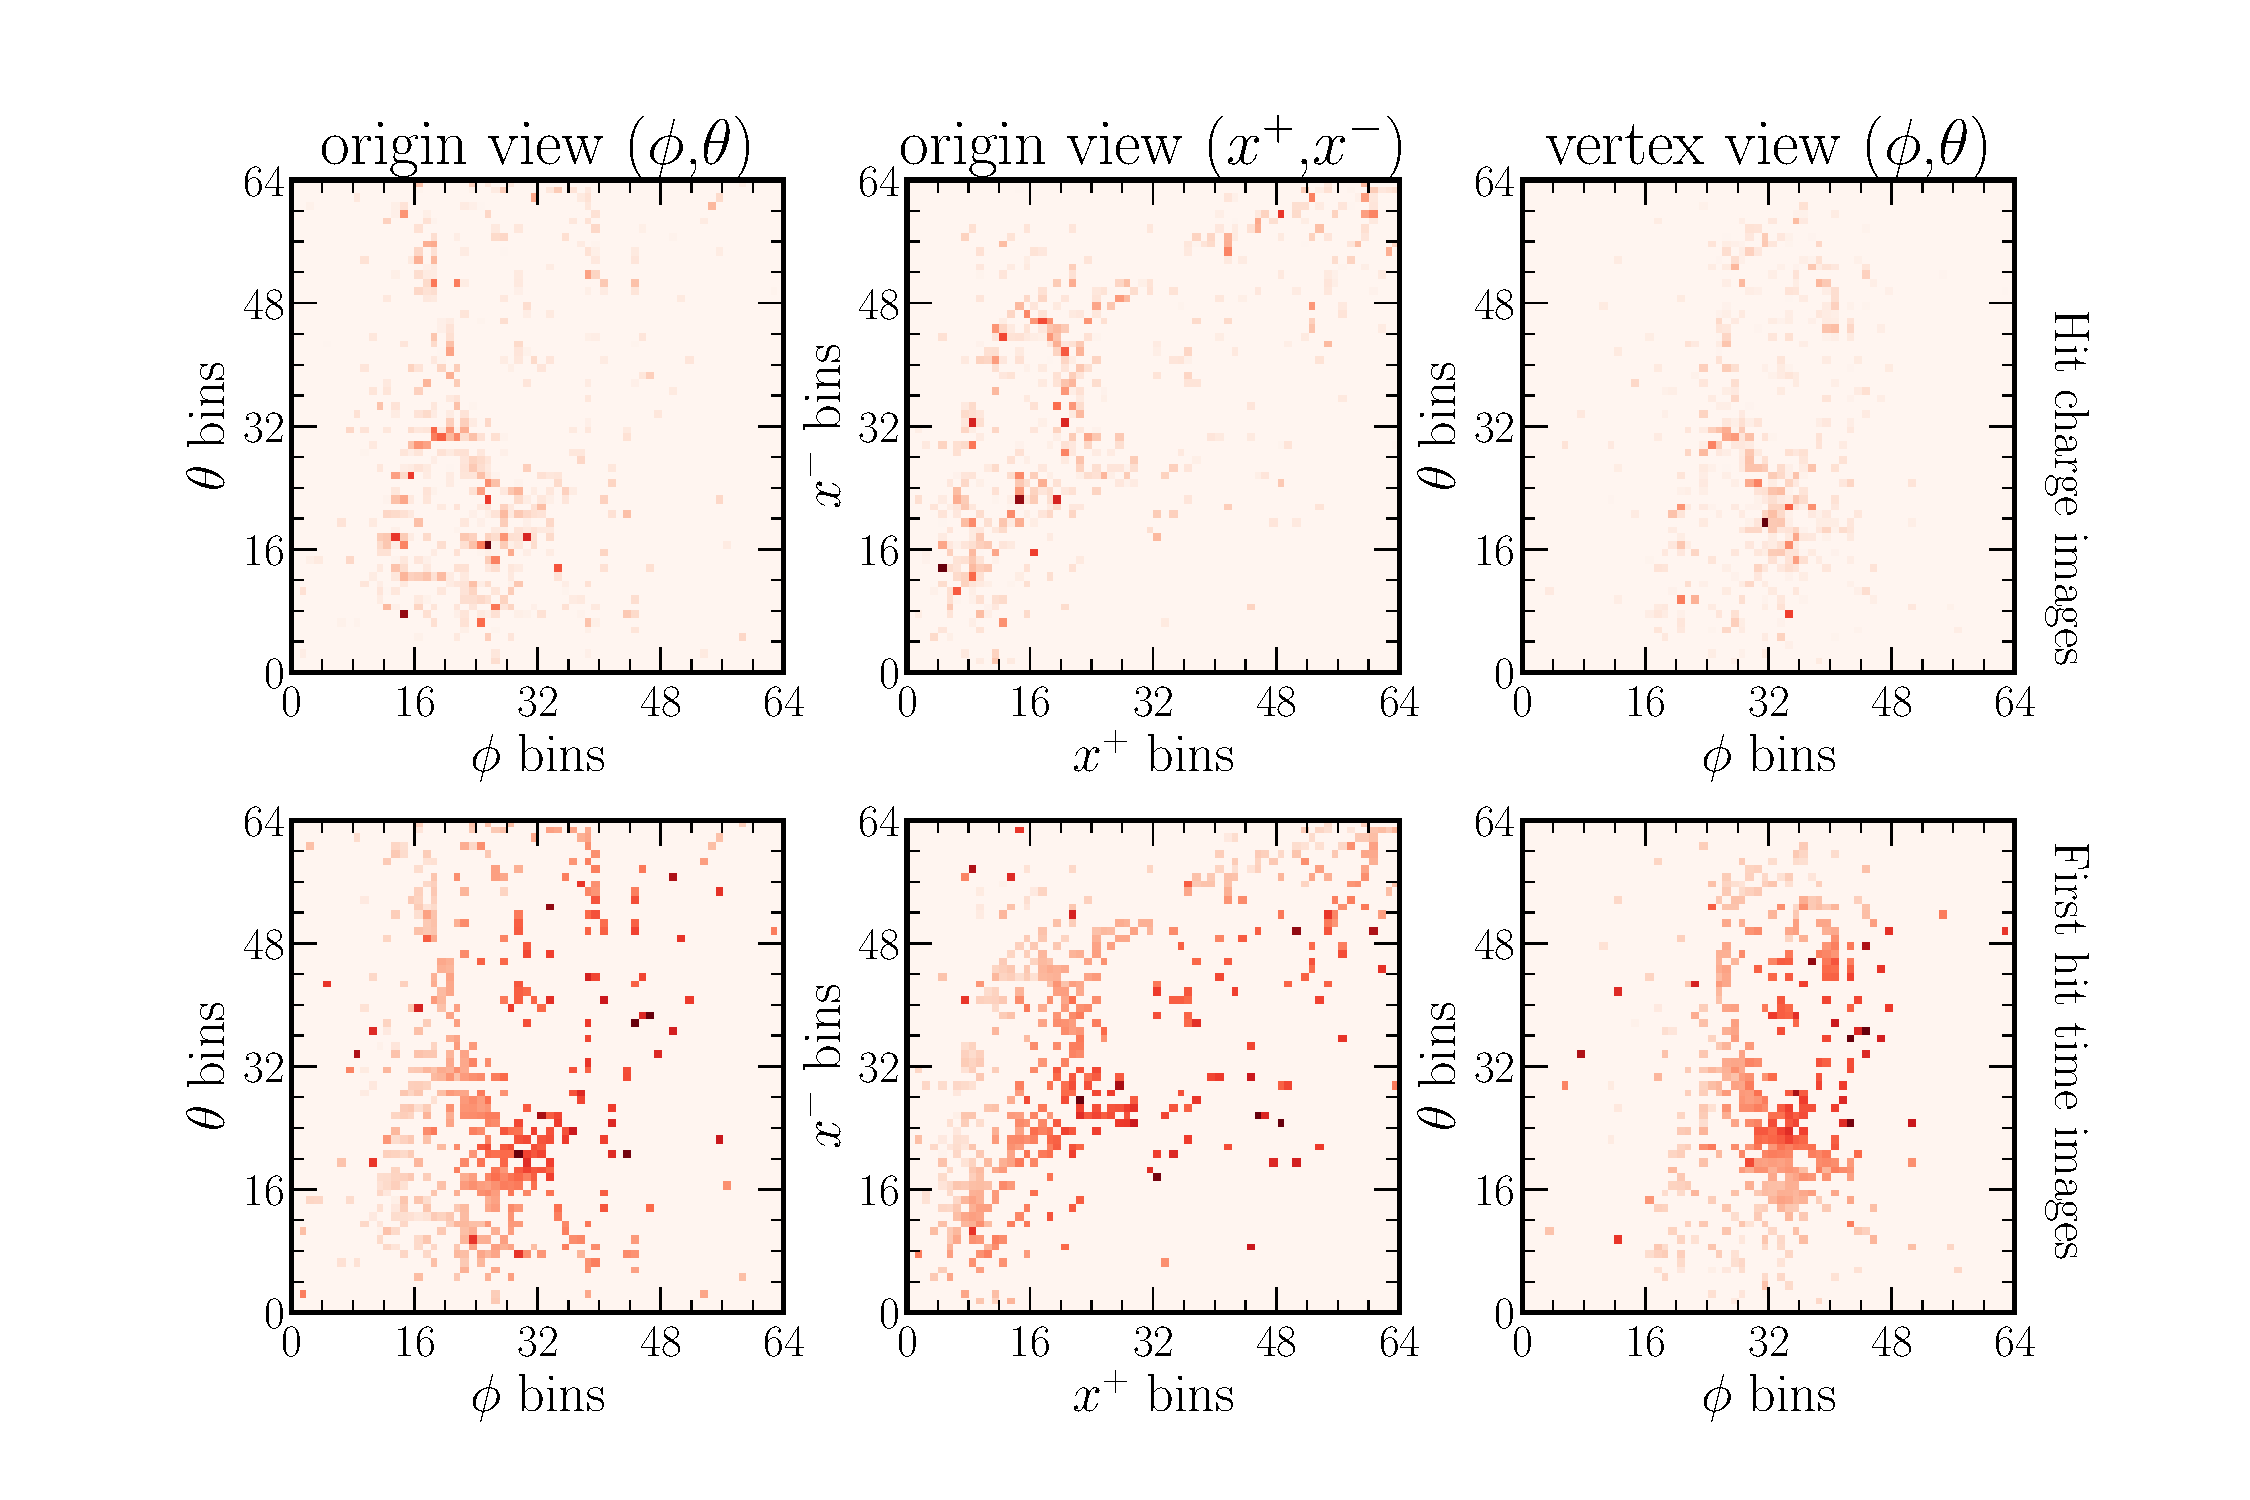
\includegraphics[width=0.8\textwidth]{diagrams/7-cvn/chipsnet/explore_numu_ccdis_event.pdf}
    \caption[explore numu ccdis event short]
    {91
        3520.17
        1862.55
            [2212   13 2112  211  211   22 -999 -999 -999 -999 -999 -999 -999 -999
                -999 -999 -999 -999 -999 -999]
            [2022.37  1862.55  1038.34   226.973  223.71     6.32  -999.    -999.
                -999.    -999.    -999.    -999.    -999.    -999.    -999.    -999.
                -999.    -999.    -999.    -999.   ]
        0}
    \label{fig:explore_numu_ccdis_event}
\end{figure}

\begin{figure} % NC EVENT DIAGRAM %
    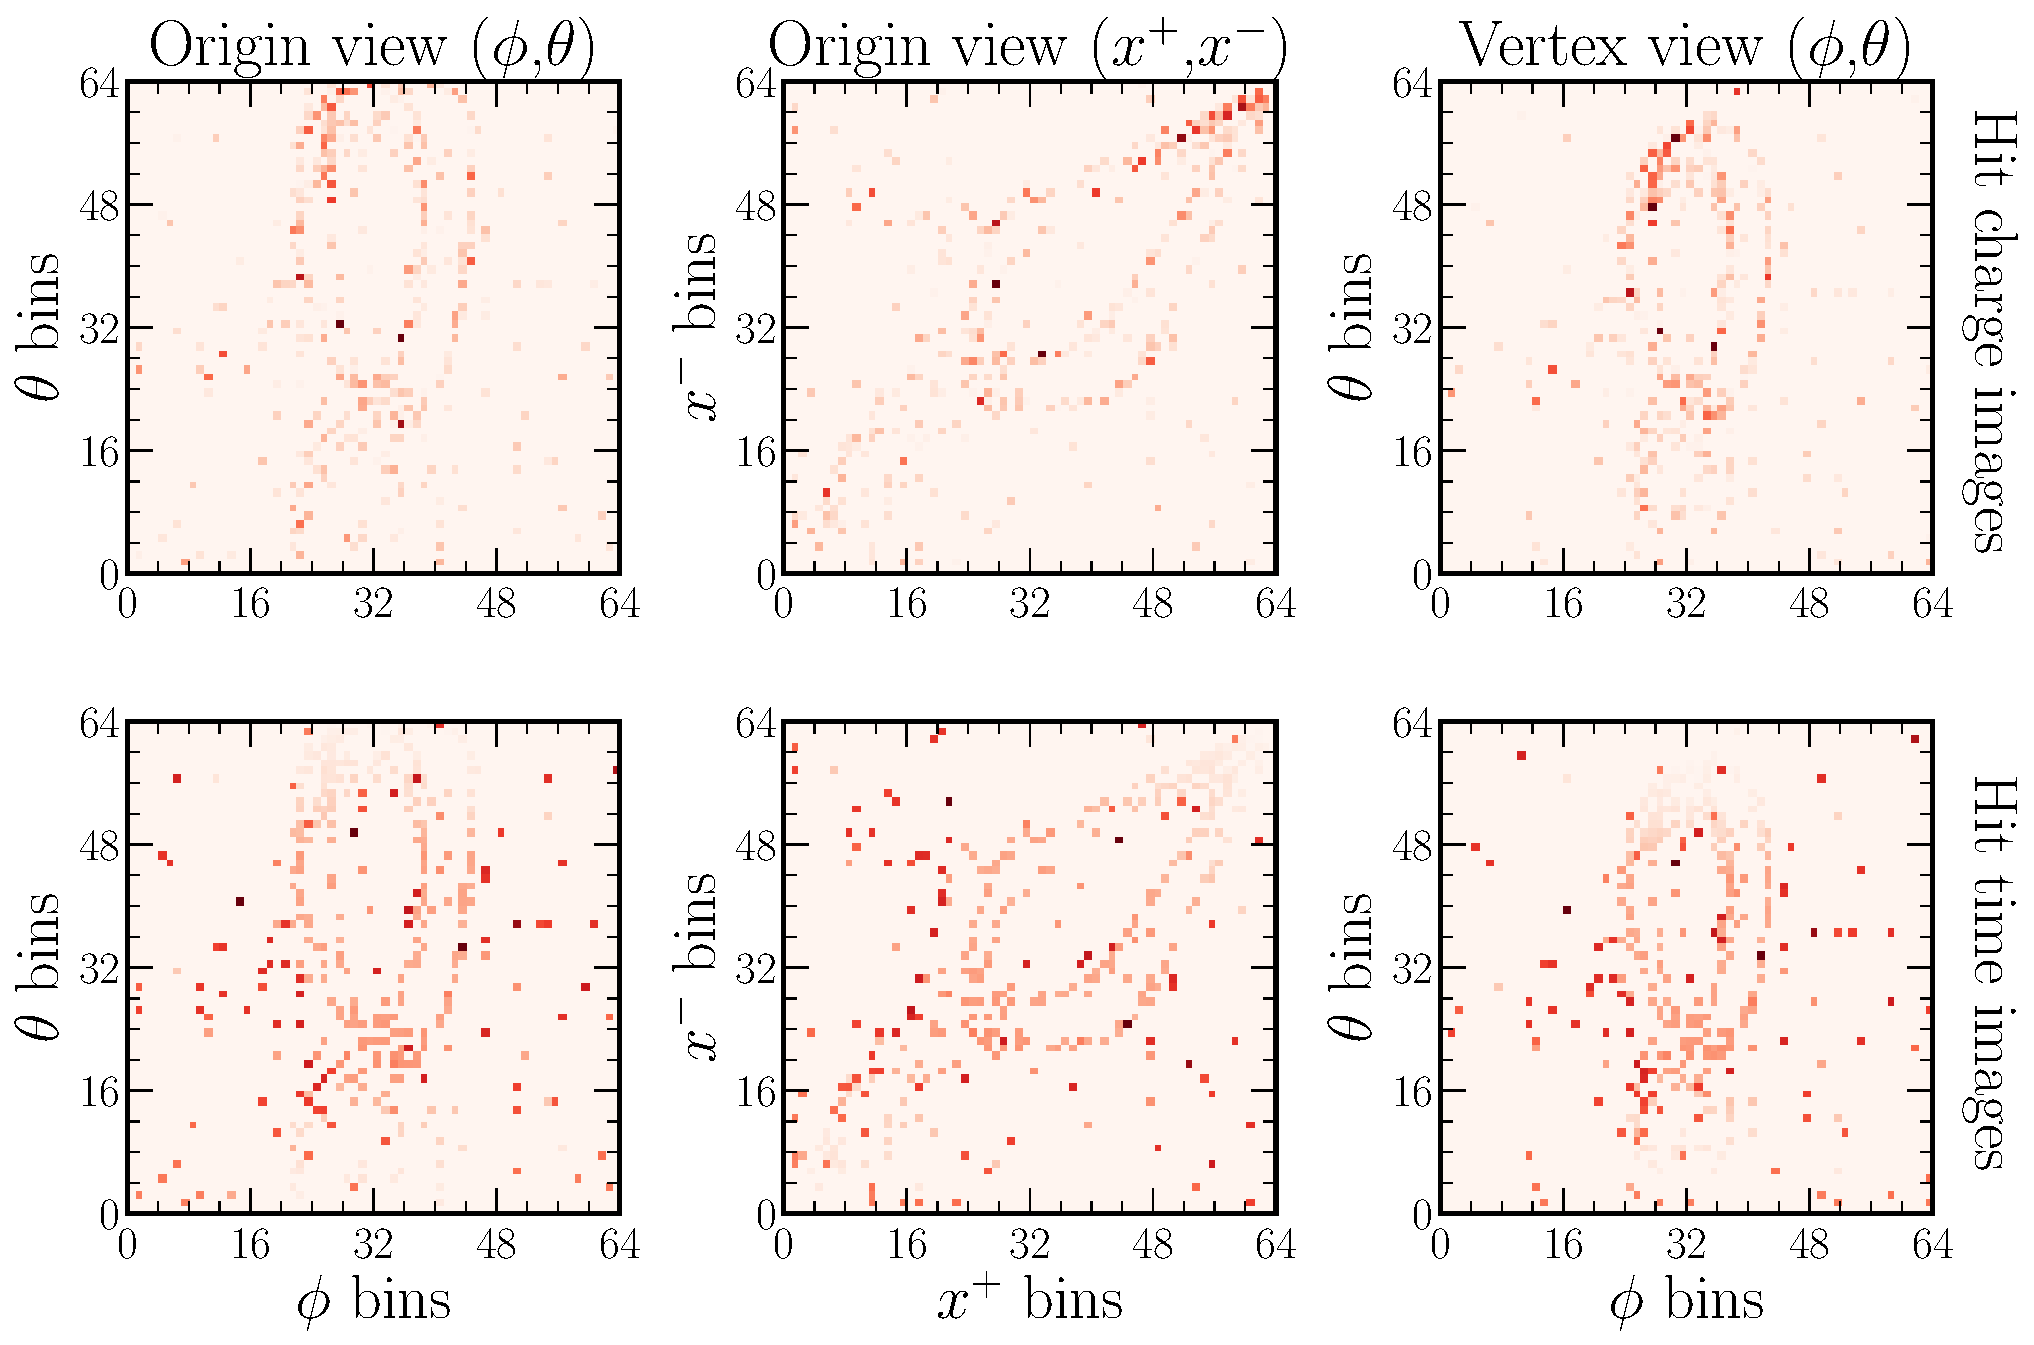
\includegraphics[width=0.8\textwidth]{diagrams/7-cvn/chipsnet/explore_nuel_ncdis_event.pdf}
    \caption[explore nuel ncdis event short]
    {92
    9301.59
    -1.0
    [  12 2212  211 2212 2212 2112 -999 -999 -999 -999 -999 -999 -999 -999
    -999 -999 -999 -999 -999 -999]
    [4731.25  2635.15  2511.54  1046.97   998.676  993.868 -999.    -999.
    -999.    -999.    -999.    -999.    -999.    -999.    -999.    -999.
    -999.    -999.    -999.    -999.   ]
    -1
    }
    \label{fig:explore_nuel_ncdis_event}
\end{figure}

\begin{figure} % COSMIC MUON EVENT DIAGRAM %
    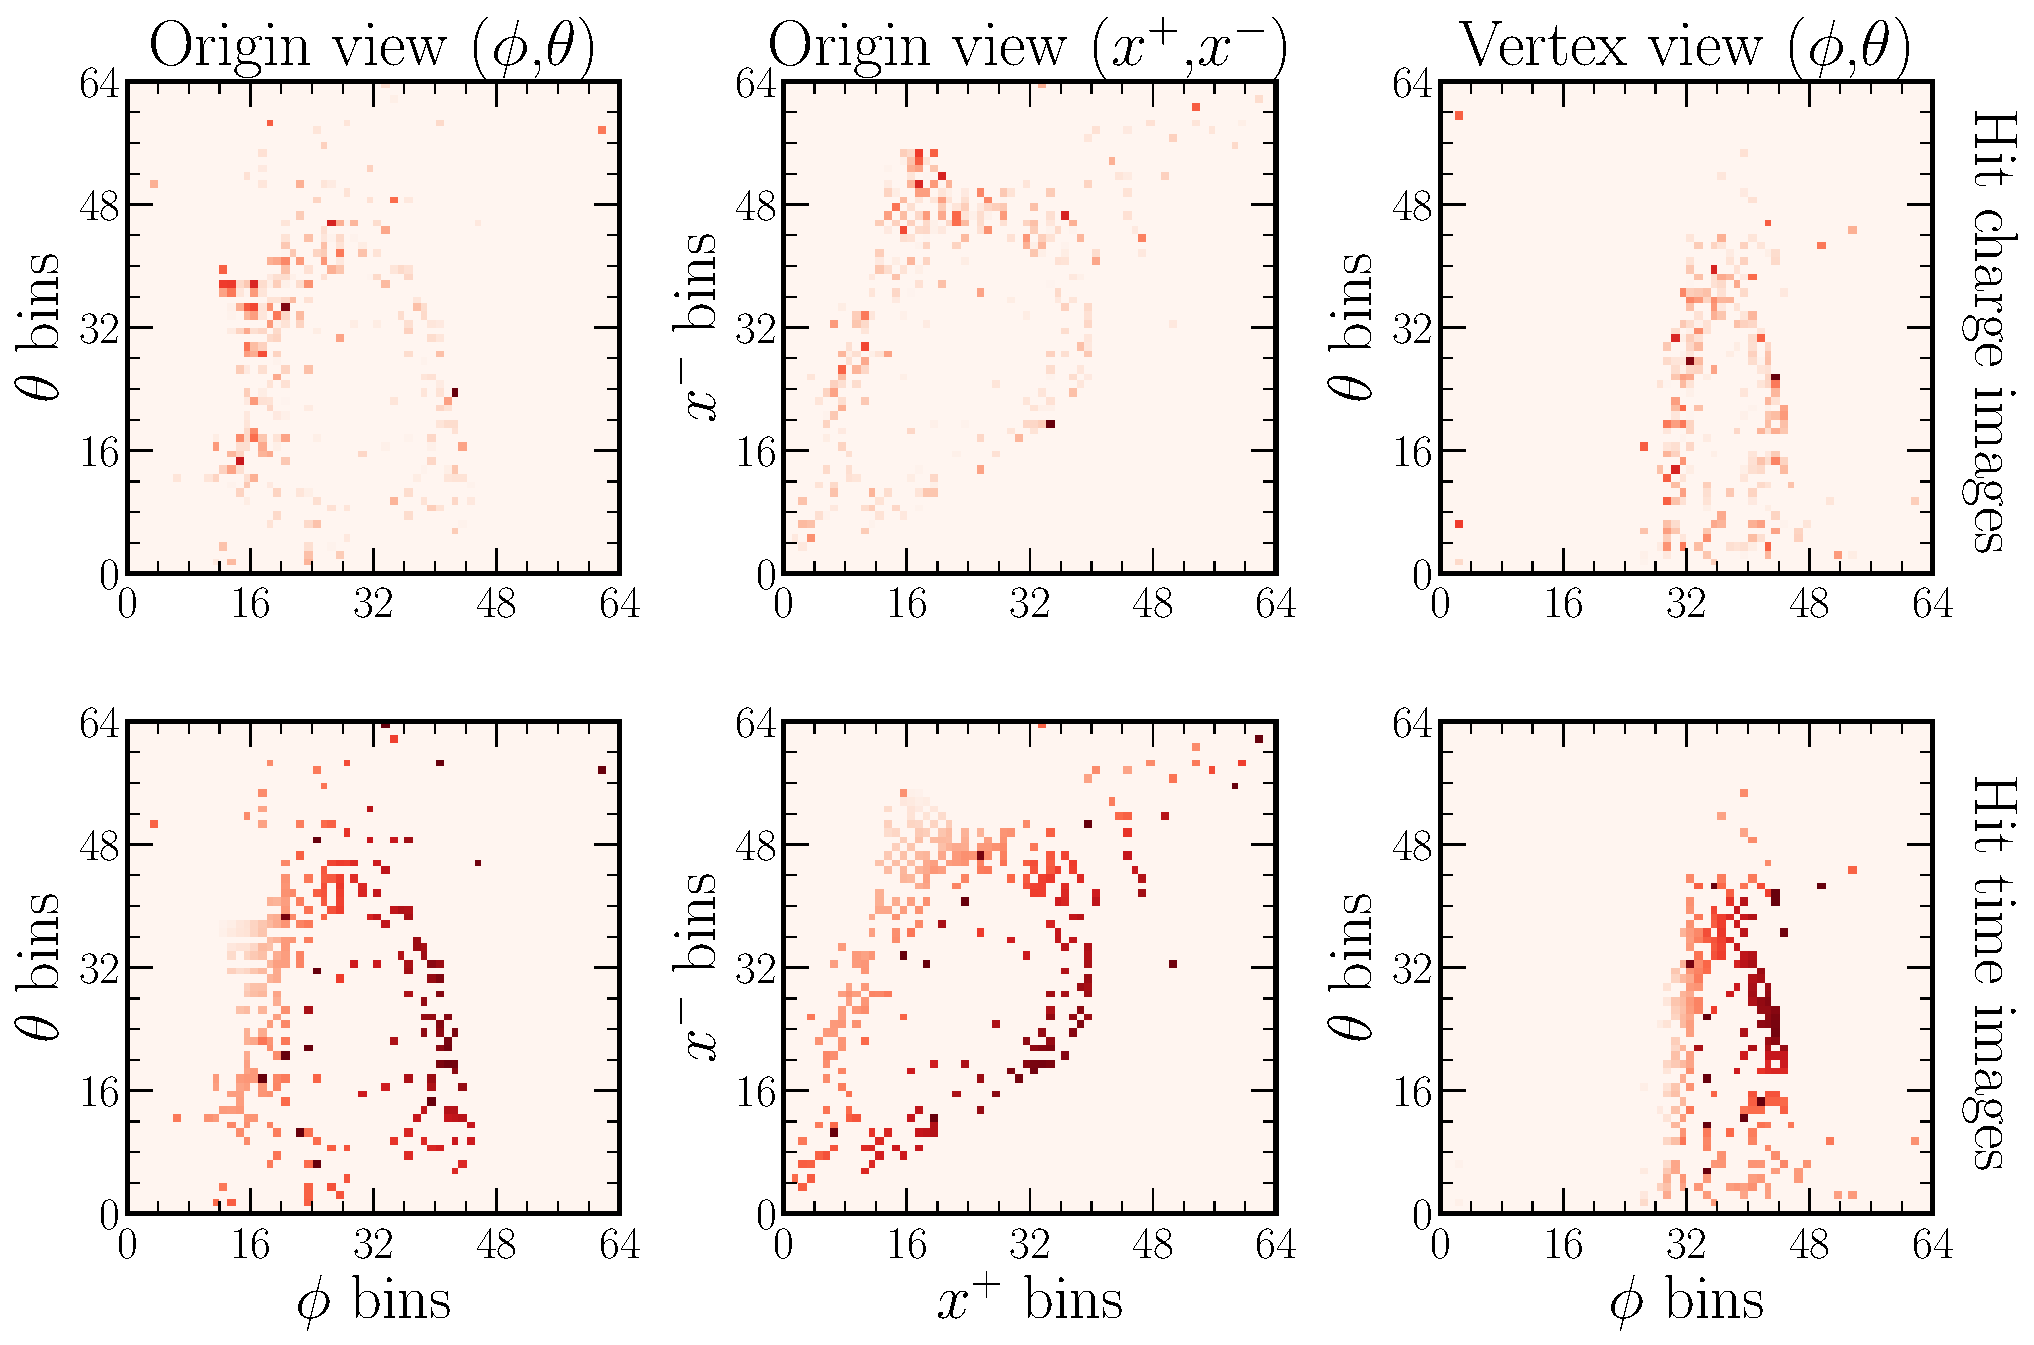
\includegraphics[width=0.8\textwidth]{diagrams/7-cvn/chipsnet/explore_cosmic_event.pdf}
    \caption[explore cosmic event short]
    {100
        2928.5
        2928.5
            [  13 -999 -999 -999 -999 -999 -999 -999 -999 -999 -999 -999 -999 -999
                -999 -999 -999 -999 -999 -999]
            [2928.5 -999.  -999.  -999.  -999.  -999.  -999.  -999.  -999.  -999.
                -999.  -999.  -999.  -999.  -999.  -999.  -999.  -999.  -999.  -999. ]
        0}
    \label{fig:explore_cosmic_event}
\end{figure}

\begin{figure} % HOUGH REPRESENTATIONS DIAGRAM %
    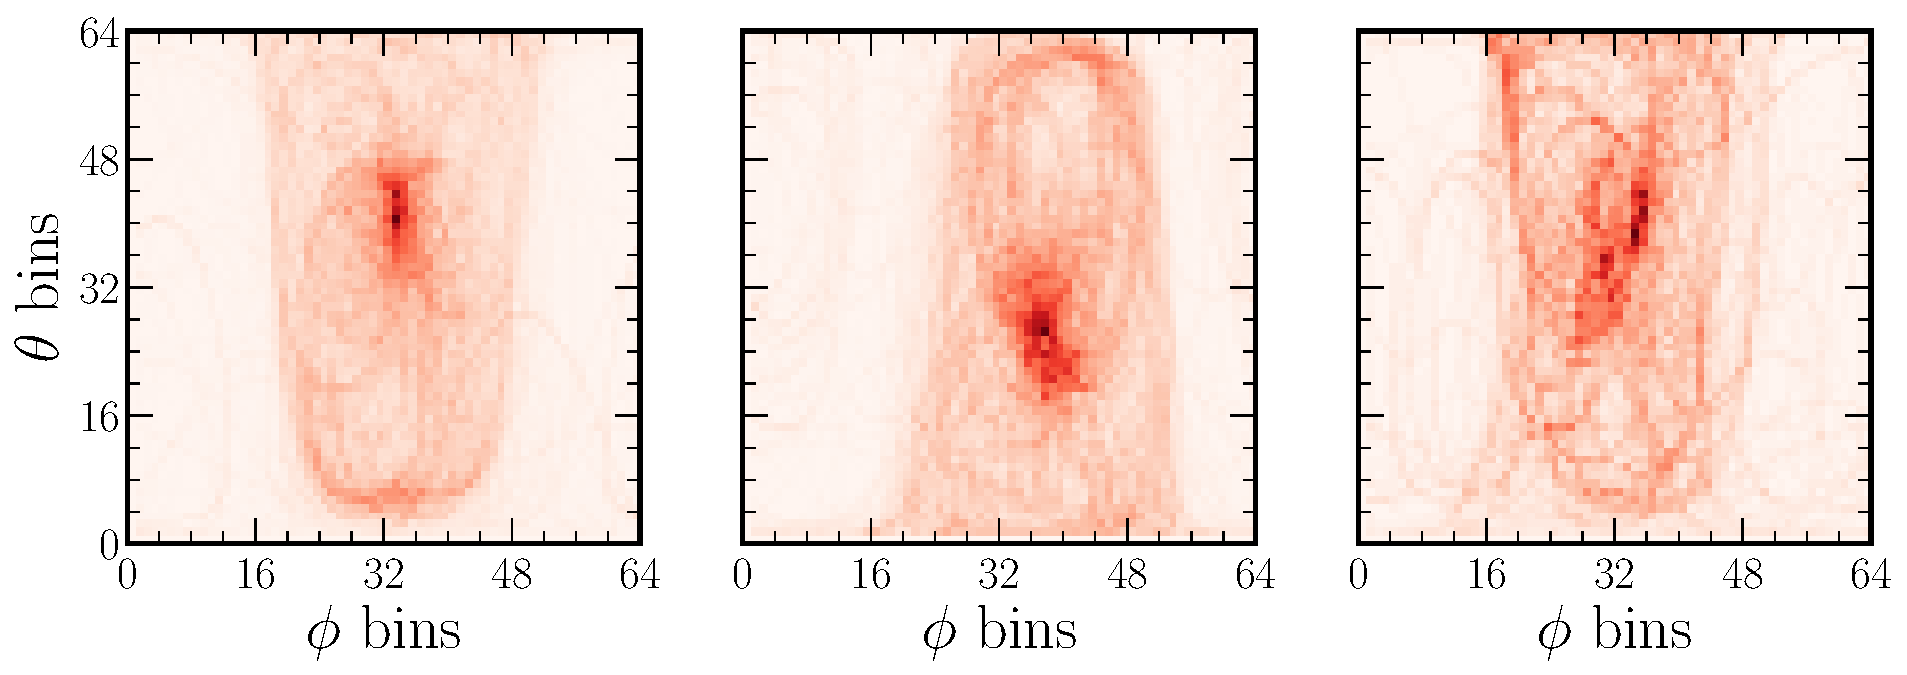
\includegraphics[width=\textwidth]{diagrams/7-cvn/chipsnet/explore_hough_events.pdf}
    \caption[example hough events short]
    {example hough events long}
    \label{fig:example_hough_events}
\end{figure}

\begin{figure} % VTX POSITIONS DIAGRAM %
    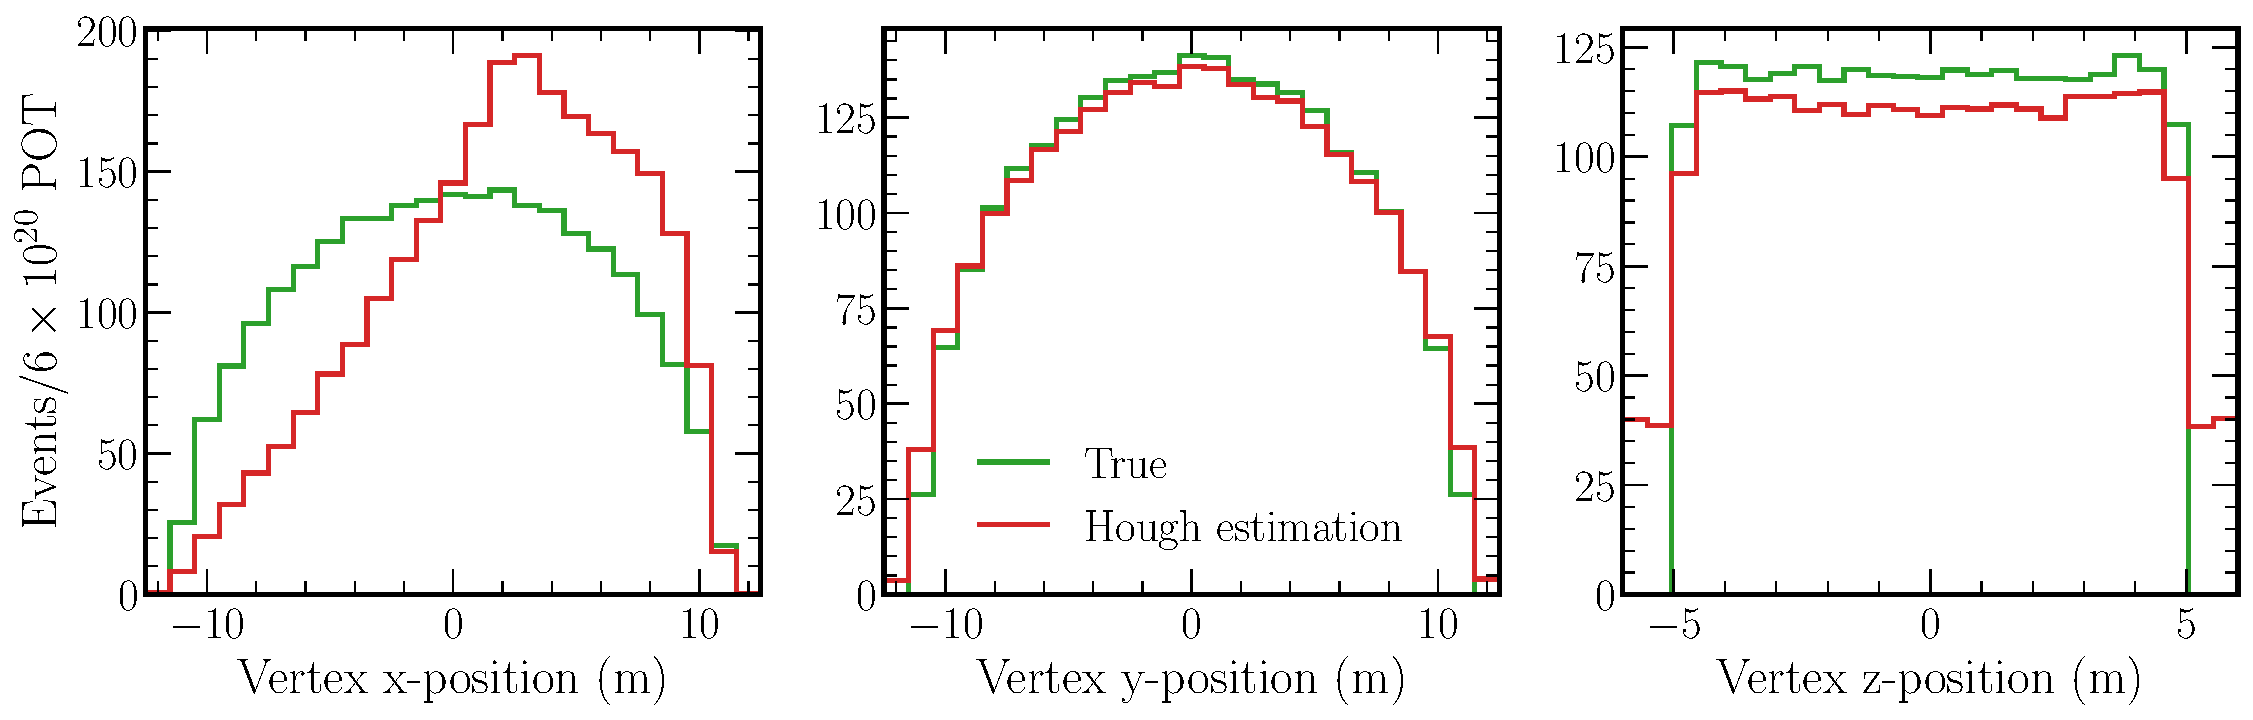
\includegraphics[width=\textwidth]{diagrams/7-cvn/chipsnet/explore_vtx_positions.pdf}
    \caption[explore vtx positions short]
    {explore vtx positions long}
    \label{fig:explore_vtx_positions}
\end{figure}

\begin{figure} % HOUGH VTX RES DIAGRAM %
    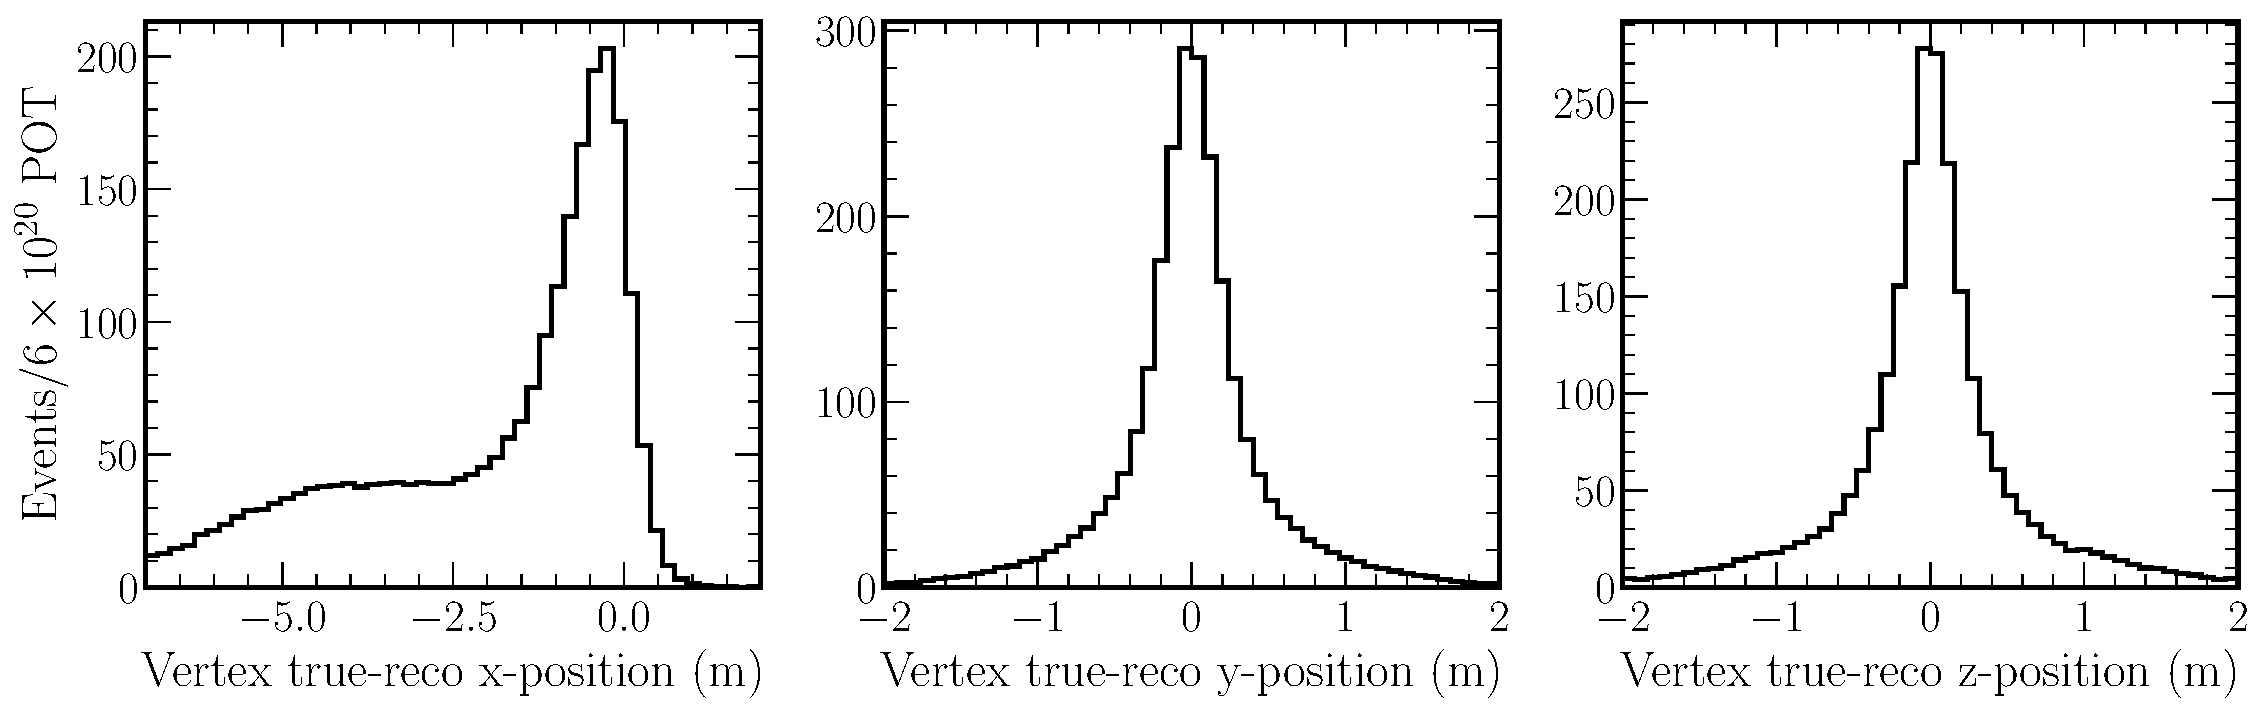
\includegraphics[width=\textwidth]{diagrams/7-cvn/chipsnet/explore_true_reco_vtx.pdf}
    \caption[explore true reco vtx short]
    {explore true reco vtx long}
    \label{fig:explore_true_reco_vtx}
\end{figure}

- Nuel-> ROC-AUC: 0.82509, PRC-AUC: 0.70686, S-Eff: 0.87786, S-Pur: 0.35433
- FOM1-> 0.46118, 0.93000, 52.98765, 8.61419, 15.27335, 0.66908, 0.68927
- FOM2-> 13.26595, 0.98500, 29.74203, 1.43964, 3.58684, 0.37556, 0.85543

- Nuel-> ROC-AUC: 0.82178, PRC-AUC: 0.67486, S-Eff: 0.87439, S-Pur: 0.29114
- FOM1-> 0.42202, 0.95500, 50.65626, 10.27209, 15.82963, 0.63948, 0.65995
- FOM2-> 12.53864, 0.99000, 29.40728, 1.75353, 3.74706, 0.37123, 0.84243

- Nuel-> ROC-AUC: 0.82116, PRC-AUC: 0.66987, S-Eff: 0.86660, S-Pur: 0.29764
- FOM1-> 0.41895, 0.94500, 50.97483, 10.86474, 16.45768, 0.64350, 0.65104
- FOM2-> 12.22739, 0.99000, 28.43808, 1.74364, 3.66555, 0.35900, 0.84019

\begin{figure} % REPR NUEL EFF CURVES DIAGRAM %
    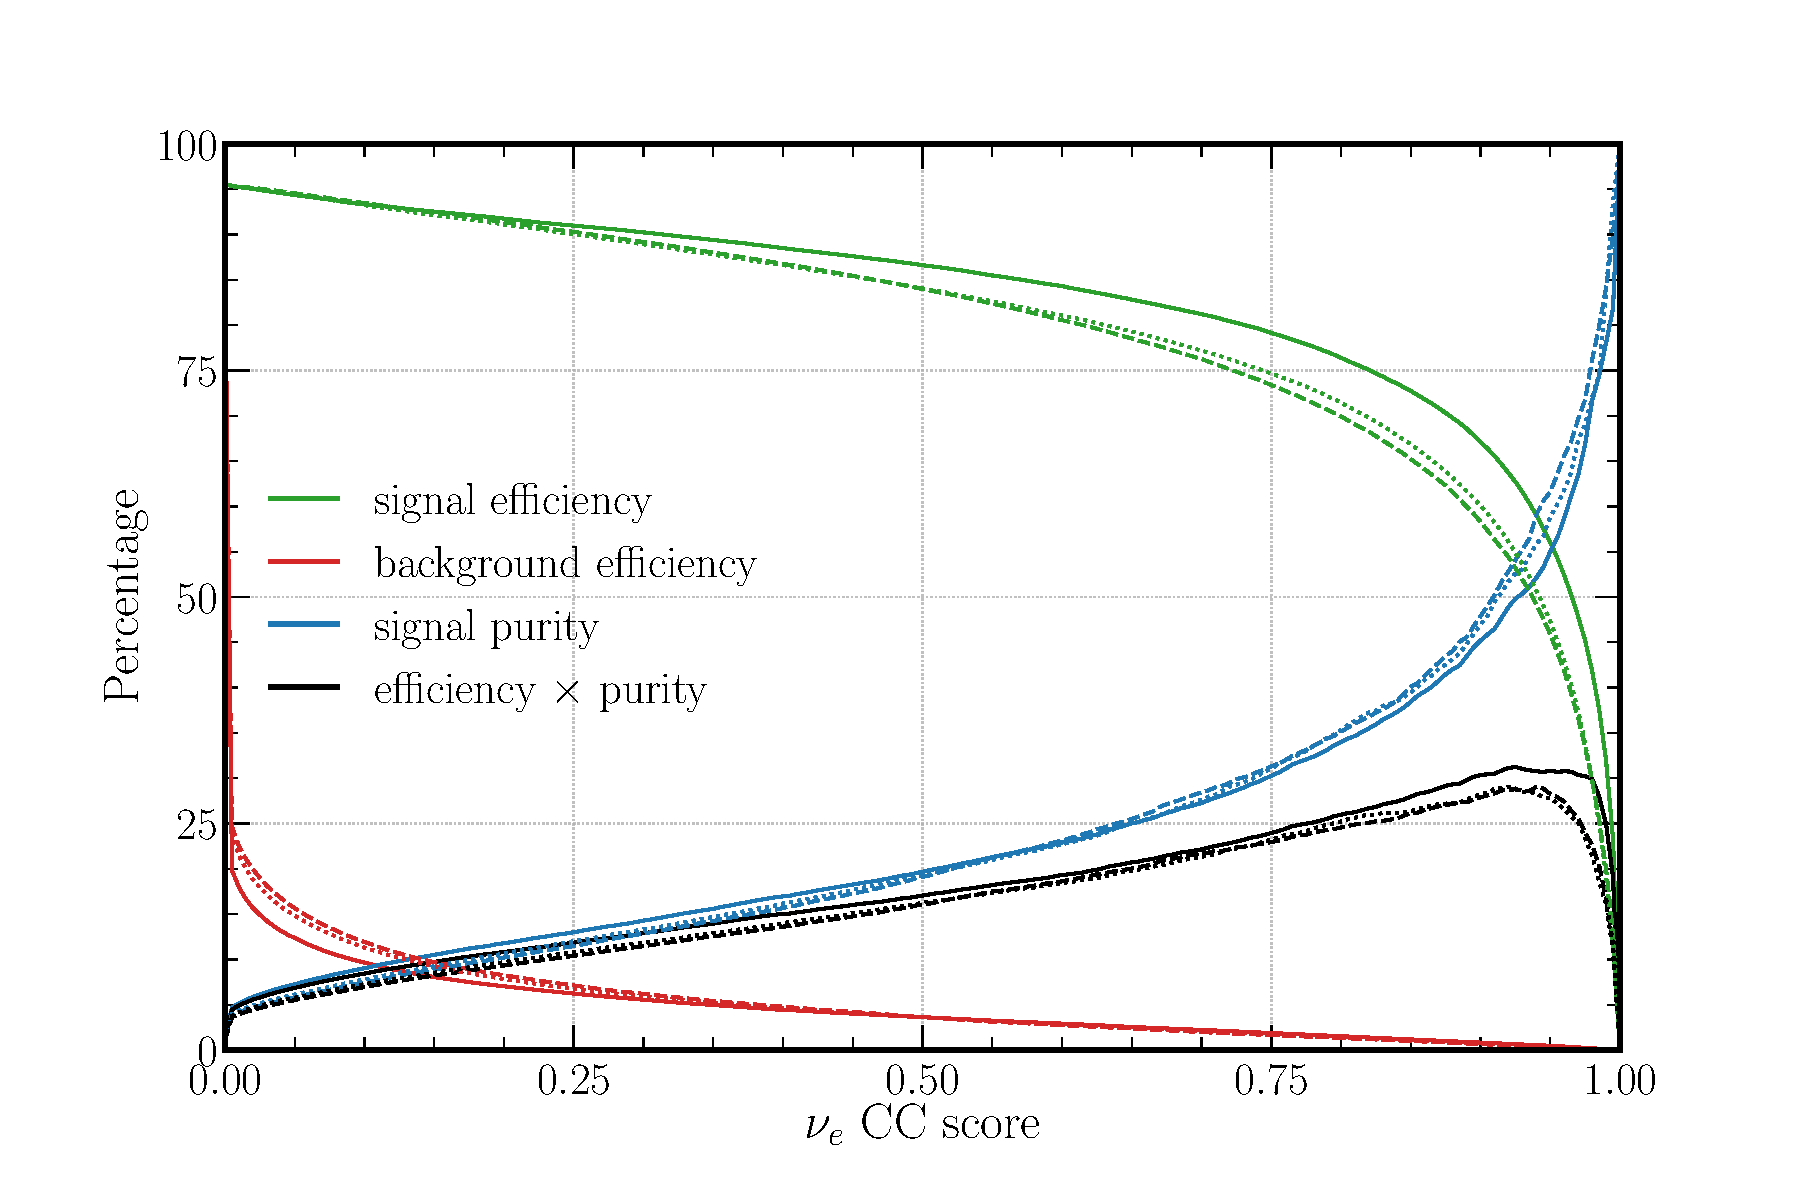
\includegraphics[width=0.6\textwidth]{diagrams/7-cvn/chipsnet/repr_nuel_eff_curves.pdf}
    \caption[repr nuel eff curves short]
    {v=solid, o=dashed, i=dotted}
    \label{fig:repr_nuel_eff_curves}
\end{figure}

\begin{figure} % REPR NUEL COMP CURVES DIAGRAM %
    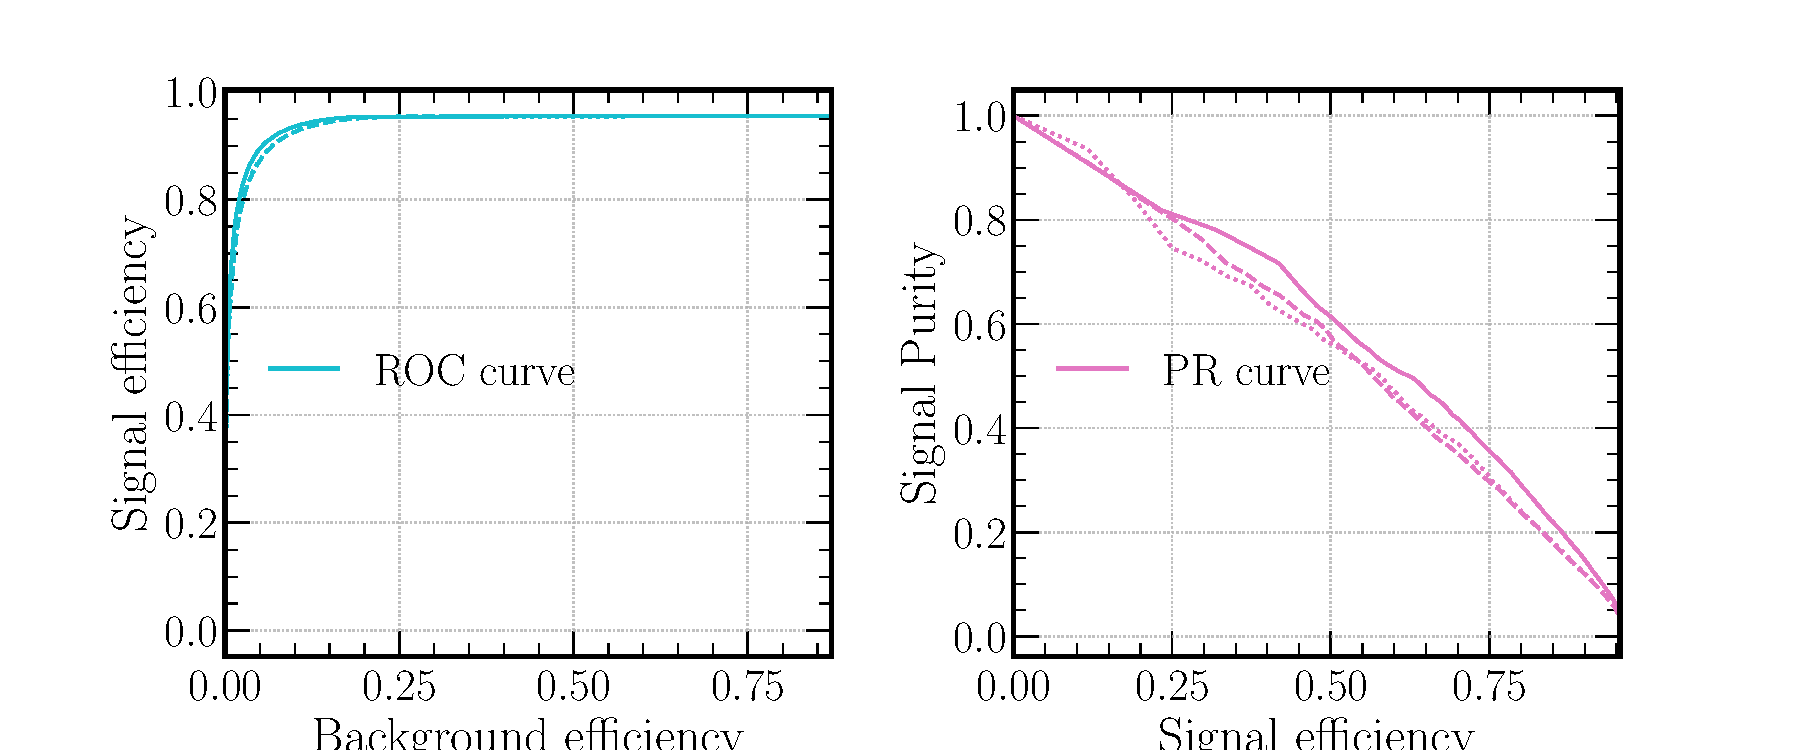
\includegraphics[width=0.8\textwidth]{diagrams/7-cvn/chipsnet/repr_nuel_comp_curves.pdf}
    \caption[repr nuel comp curves short]
    {v=solid, o=dashed, i=dotted}
    \label{fig:repr_nuel_comp_curves}
\end{figure}

\begin{figure} % REPR NUMU EFF CURVES DIAGRAM %
    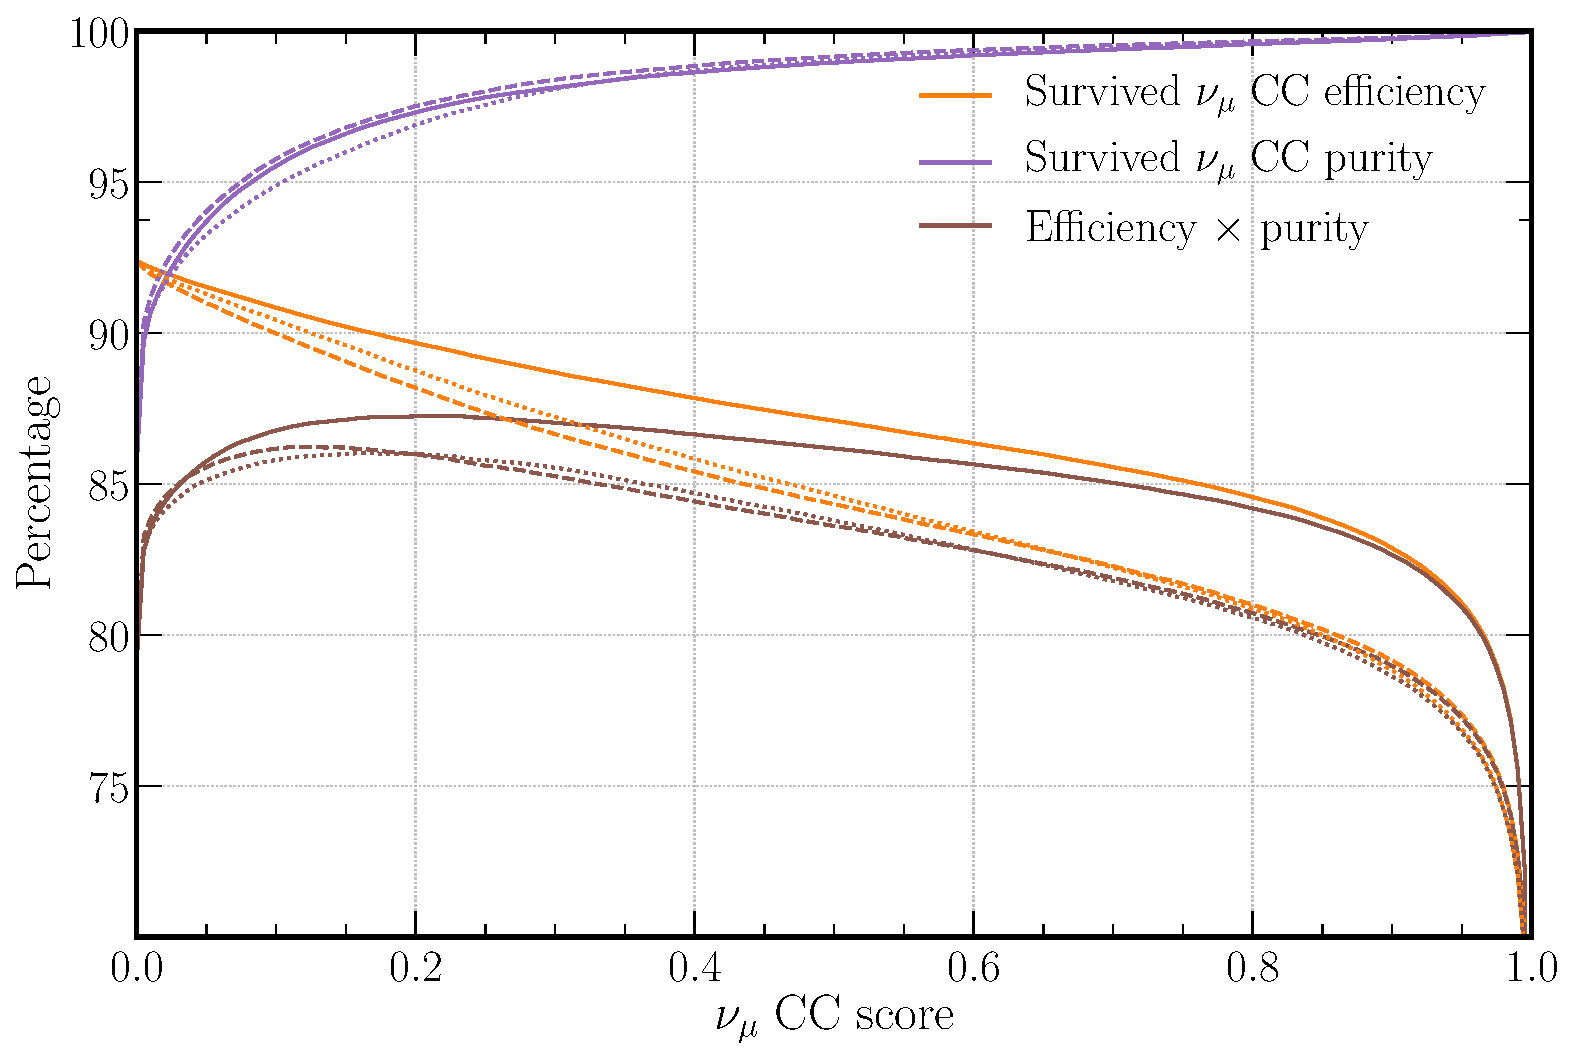
\includegraphics[width=0.6\textwidth]{diagrams/7-cvn/chipsnet/repr_numu_eff_curves.pdf}
    \caption[repr numu eff curves short]
    {v=solid, o=dashed, i=dotted}
    \label{fig:repr_numu_eff_curves}
\end{figure}

\begin{figure} % REPR NUMU COMP CURVES DIAGRAM %
    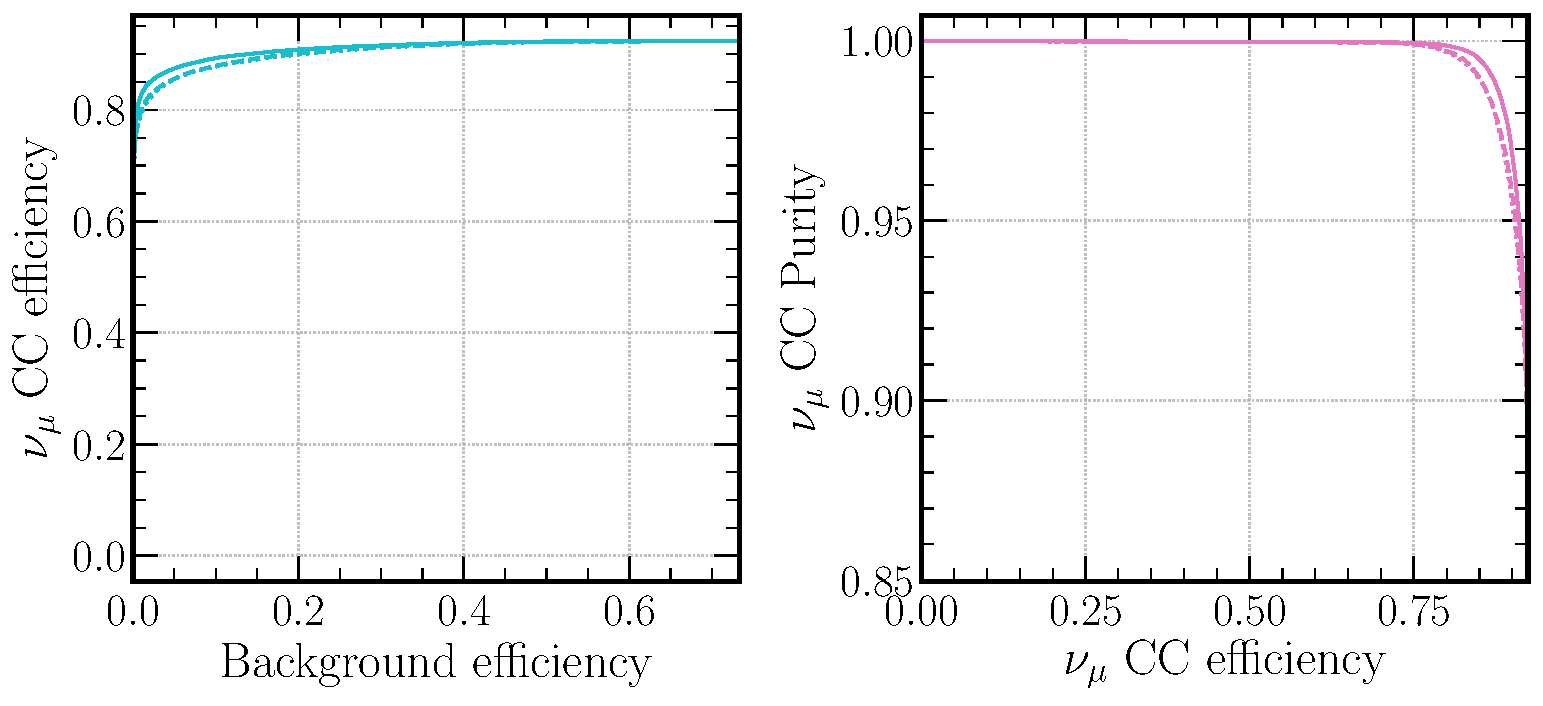
\includegraphics[width=0.8\textwidth]{diagrams/7-cvn/chipsnet/repr_numu_comp_curves.pdf}
    \caption[repr numu comp curves short]
    {v=solid, o=dashed, i=dotted}
    \label{fig:repr_numu_comp_curves}
\end{figure}

\subsection{Which channels to use} %%%%%%%%%%%%%%%%%%%%%%%%%%%%%%%%%%%%%%%%%%%%%%%%%%%%%%%%%%%%%%%
\label{sec:cvn_baseline_channel} %%%%%%%%%%%%%%%%%%%%%%%%%%%%%%%%%%%%%%%%%%%%%%%%%%%%%%%%%%%%%%%%%

\begin{figure} % CHANNEL NUEL EFF CURVES DIAGRAM %
    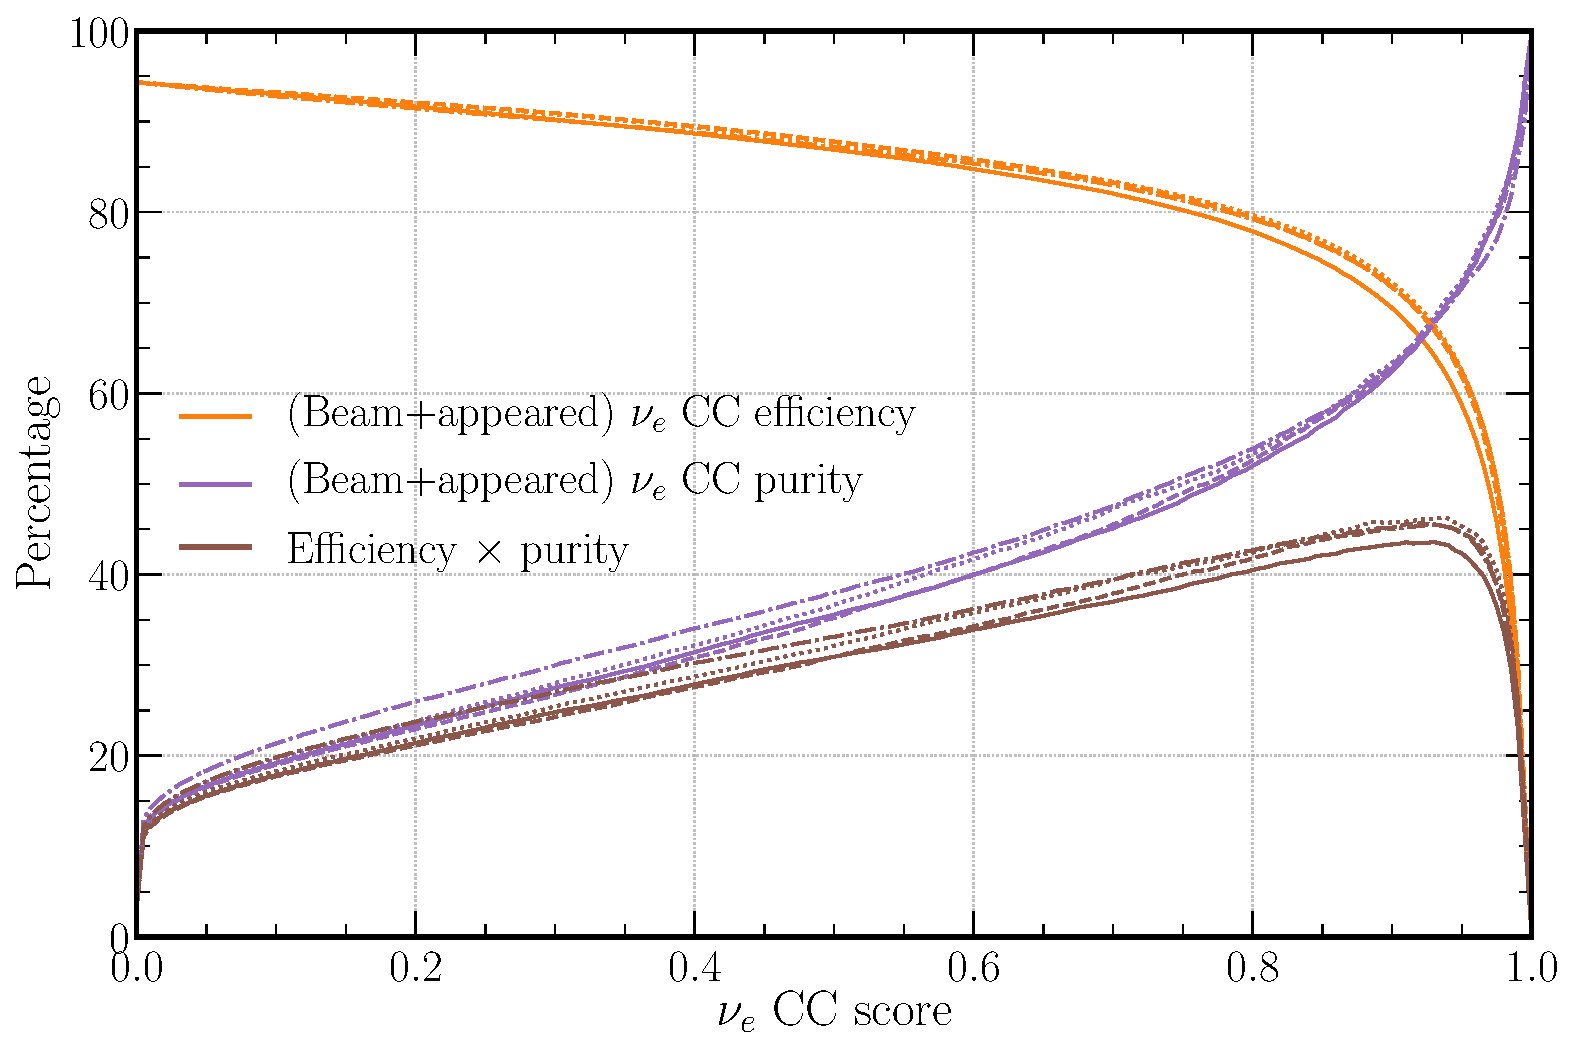
\includegraphics[width=0.6\textwidth]{diagrams/7-cvn/chipsnet/channel_nuel_eff_curves.pdf}
    \caption[channel nuel eff curves short]
    {c=solid, ct=dashed, cth=dotted, cth-stacked=dot-dash}
    \label{fig:channel_nuel_eff_curves}
\end{figure}

\begin{figure} % CHANNEL NUEL COMP CURVES DIAGRAM %
    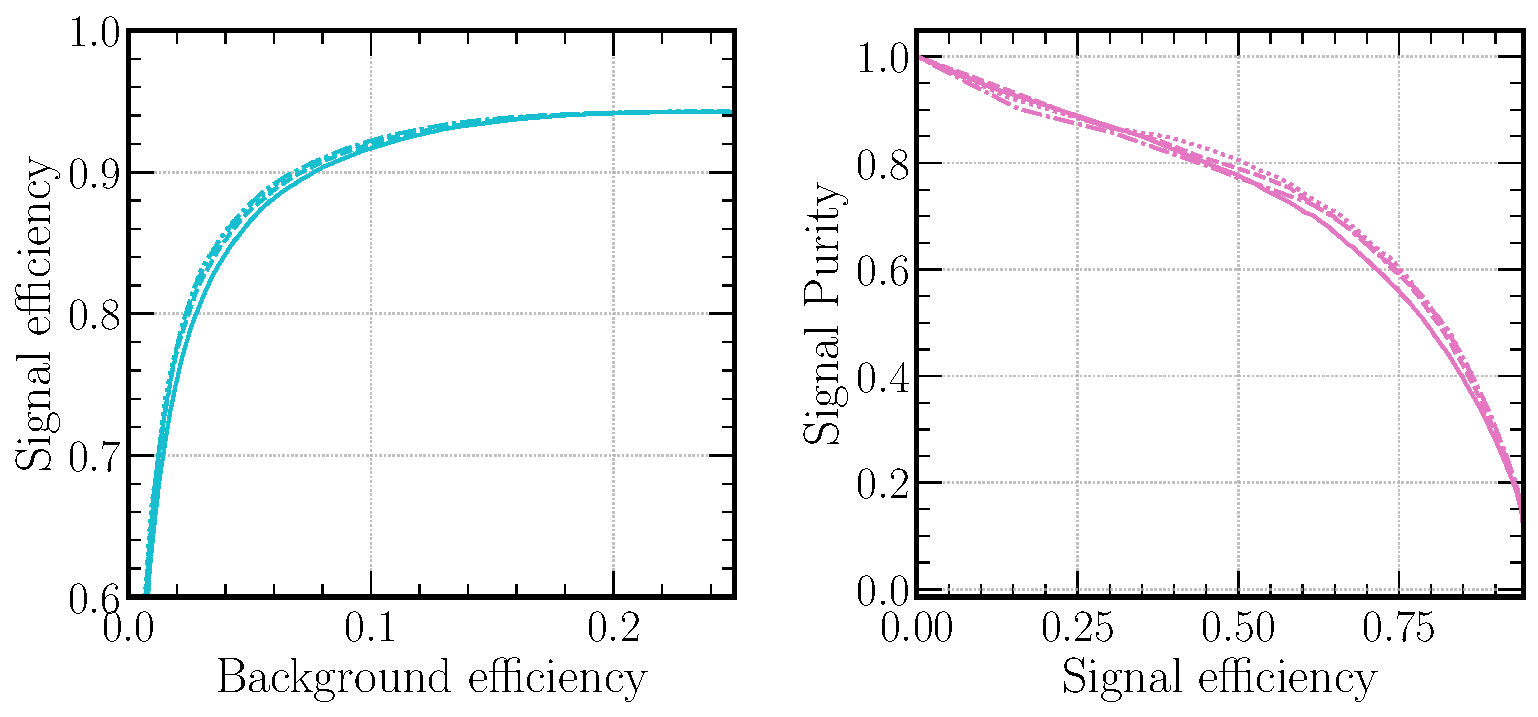
\includegraphics[width=0.8\textwidth]{diagrams/7-cvn/chipsnet/channel_nuel_comp_curves.pdf}
    \caption[channel nuel comp curves short]
    {c=solid, ct=dashed, cth=dotted, cth-stacked=dot-dash}
    \label{fig:channel_nuel_comp_curves}
\end{figure}

- Nuel-> ROC-AUC: 0.82377, PRC-AUC: 0.68935, S-Eff: 0.86860, S-Pur: 0.35681
- FOM1-> 0.43601, 0.91000, 53.71070, 12.22704, 17.60798, 0.67821, 0.64289
- FOM2-> 12.70378, 0.99000, 20.73912, 0.76294, 1.90217, 0.26187, 0.88613

- Nuel-> ROC-AUC: 0.82509, PRC-AUC: 0.70686, S-Eff: 0.87786, S-Pur: 0.35433
- FOM1-> 0.46118, 0.93000, 52.98765, 8.61419, 15.27335, 0.66908, 0.68927
- FOM2-> 13.26595, 0.98500, 29.74203, 1.43964, 3.58684, 0.37556, 0.85543

- Nuel-> ROC-AUC: 0.82559, PRC-AUC: 0.71155, S-Eff: 0.87661, S-Pur: 0.36928
- FOM1-> 0.46510, 0.93000, 53.44422, 8.34671, 15.75487, 0.67485, 0.68920
- FOM2-> 13.44645, 0.98500, 31.21664, 1.57028, 3.81933, 0.39418, 0.85277

- Nuel-> ROC-AUC: 0.82521, PRC-AUC: 0.70198, S-Eff: 0.87180, S-Pur: 0.38254
- FOM1-> 0.45819, 0.91500, 55.18628, 11.56662, 17.17741, 0.69684, 0.65753
- FOM2-> 12.66558, 0.99000, 24.37959, 1.35104, 2.35408, 0.30784, 0.86807

\begin{figure} % CHANNEL NUMU EFF CURVES DIAGRAM %
    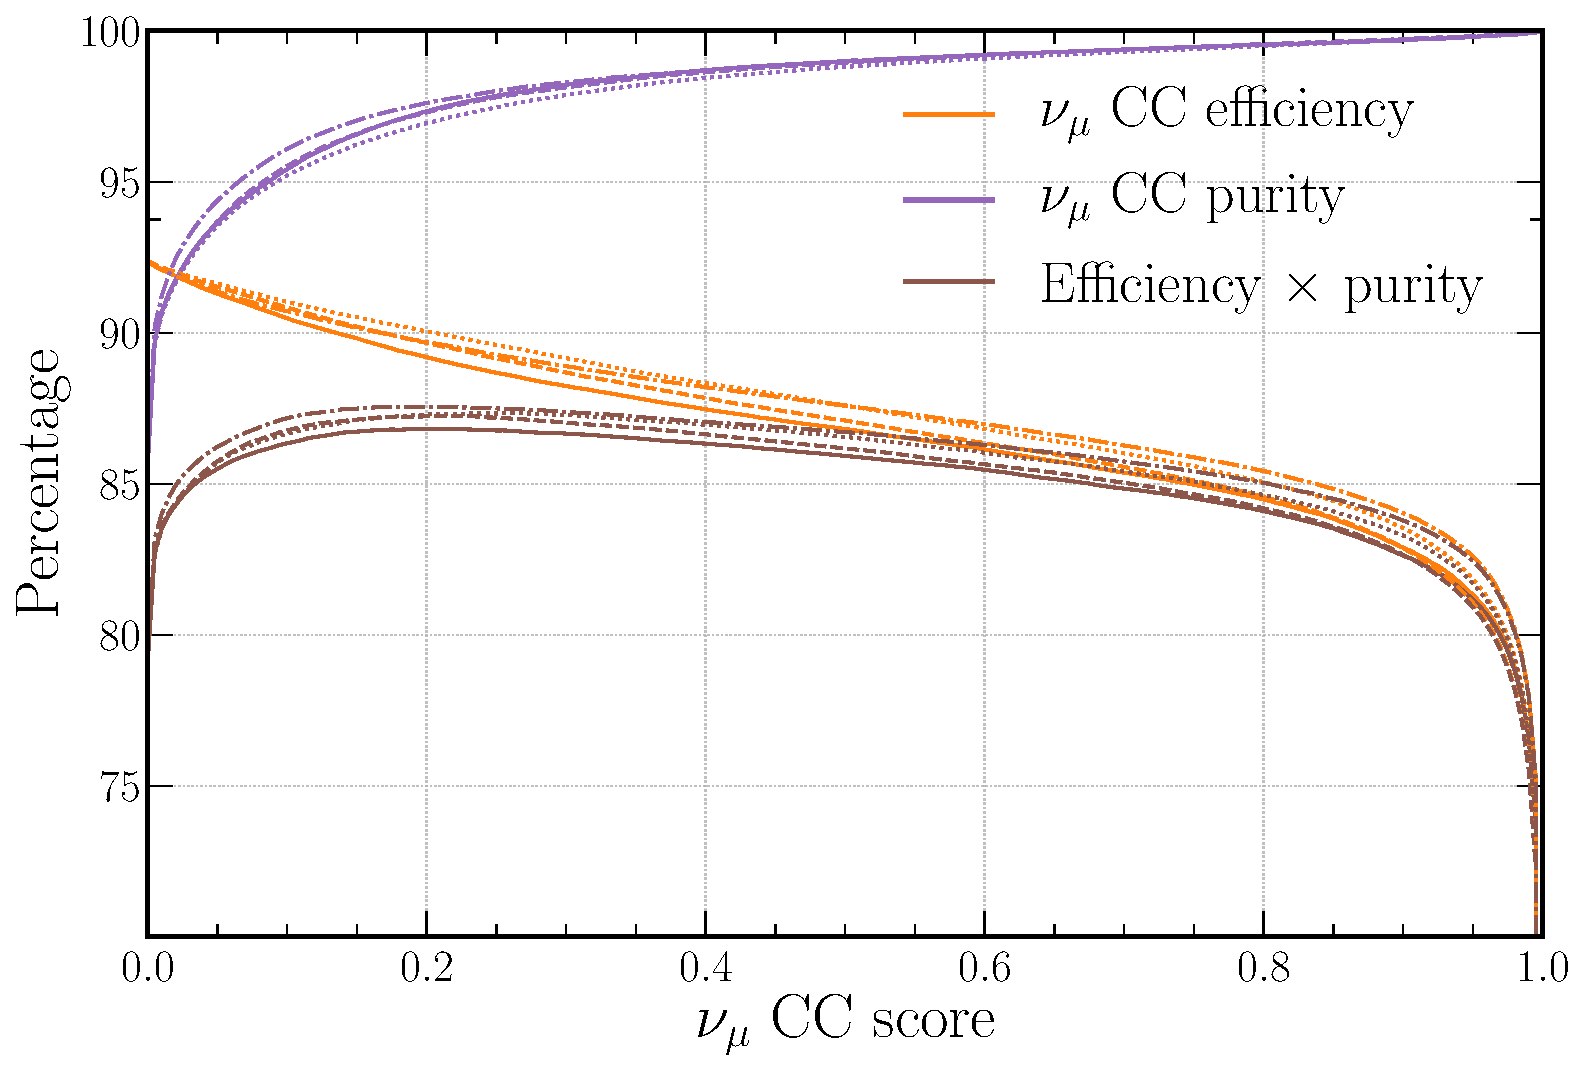
\includegraphics[width=0.6\textwidth]{diagrams/7-cvn/chipsnet/channel_numu_eff_curves.pdf}
    \caption[channel numu eff curves short]
    {c=solid, ct=dashed, cth=dotted, cth-stacked=dot-dash}
    \label{fig:channel_numu_eff_curves}
\end{figure}

\begin{figure} % CHANNEL NUMU COMP CURVES DIAGRAM %
    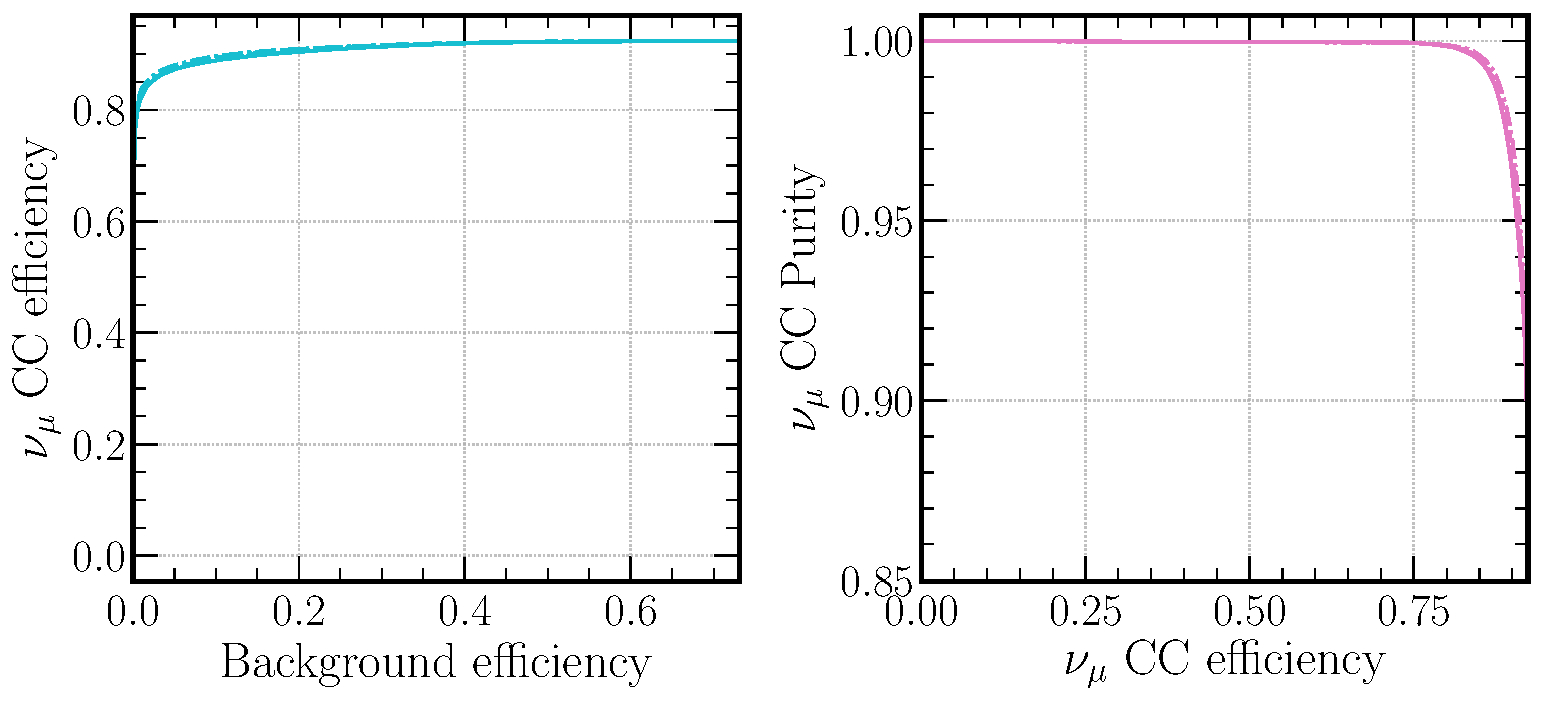
\includegraphics[width=0.8\textwidth]{diagrams/7-cvn/chipsnet/channel_numu_comp_curves.pdf}
    \caption[channel numu comp curves short]
    {c=solid, ct=dashed, cth=dotted, cth-stacked=dot-dash}
    \label{fig:channel_numu_comp_curves}
\end{figure}

\subsection{Multitask methodology} %%%%%%%%%%%%%%%%%%%%%%%%%%%%%%%%%%%%%%%%%%%%%%%%%%%%%%%%%%%%%%%
\label{sec:cvn_baseline_multi} %%%%%%%%%%%%%%%%%%%%%%%%%%%%%%%%%%%%%%%%%%%%%%%%%%%%%%%%%%%%%%%%%%%

Multi-task learning how to weight paper in Ref.~\cite{kendall2018}

\section{Cosmic muon rejection} %%%%%%%%%%%%%%%%%%%%%%%%%%%%%%%%%%%%%%%%%%%%%%%%%%%%%%%%%%%%%%%%%%
\label{sec:cvn_cosmic} %%%%%%%%%%%%%%%%%%%%%%%%%%%%%%%%%%%%%%%%%%%%%%%%%%%%%%%%%%%%%%%%%%%%%%%%%%%

\section{Beam classification} %%%%%%%%%%%%%%%%%%%%%%%%%%%%%%%%%%%%%%%%%%%%%%%%%%%%%%%%%%%%%%%%%%%%
\label{sec:cvn_beam} %%%%%%%%%%%%%%%%%%%%%%%%%%%%%%%%%%%%%%%%%%%%%%%%%%%%%%%%%%%%%%%%%%%%%%%%%%%%%

\subsection{Which categorisation to use} %%%%%%%%%%%%%%%%%%%%%%%%%%%%%%%%%%%%%%%%%%%%%%%%%%%%%%%%%
\label{sec:cvn_beam_cat} %%%%%%%%%%%%%%%%%%%%%%%%%%%%%%%%%%%%%%%%%%%%%%%%%%%%%%%%%%%%%%%%%%%%%%%%%

\begin{figure} % T_ALL_CAT SAMPLE DIAGRAM %
    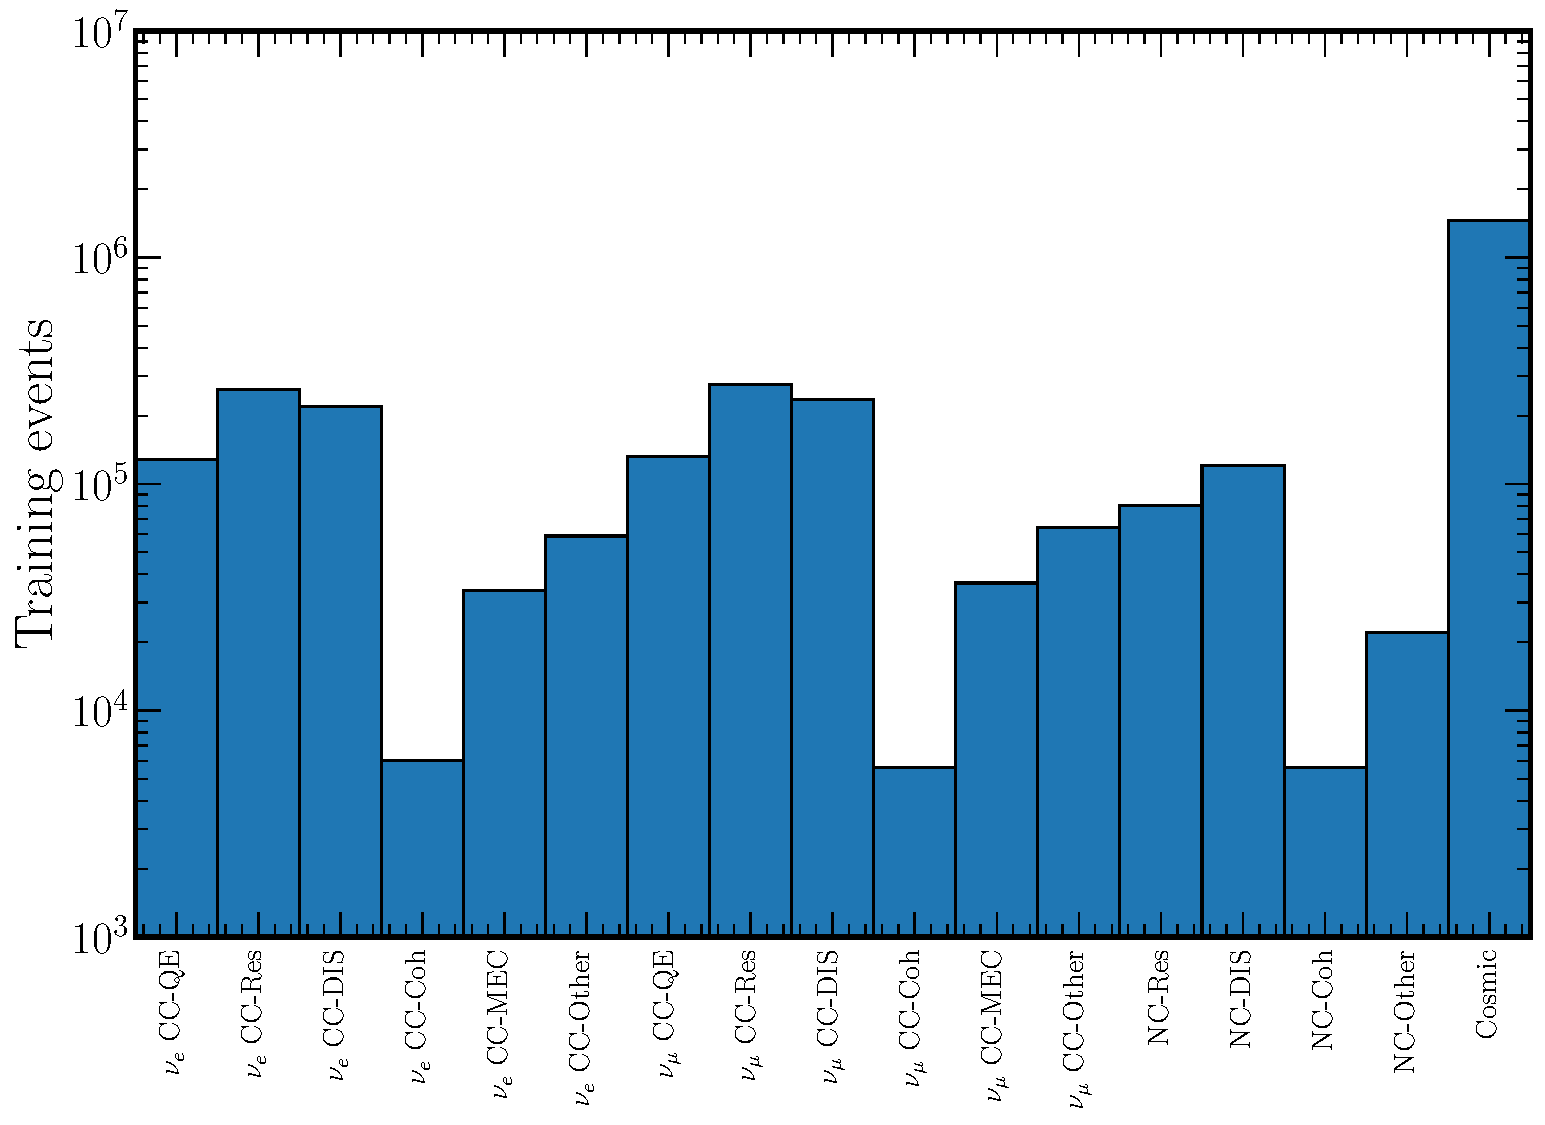
\includegraphics[width=0.6\textwidth]{diagrams/7-cvn/chipsnet/explore_t_all_cat.pdf}
    \caption[explore t all cat short]
    {explore t all cat long}
    \label{fig:explore_t_all_cat}
\end{figure}

\begin{figure} % T_NC_COMB_CAT SAMPLE DIAGRAM %
    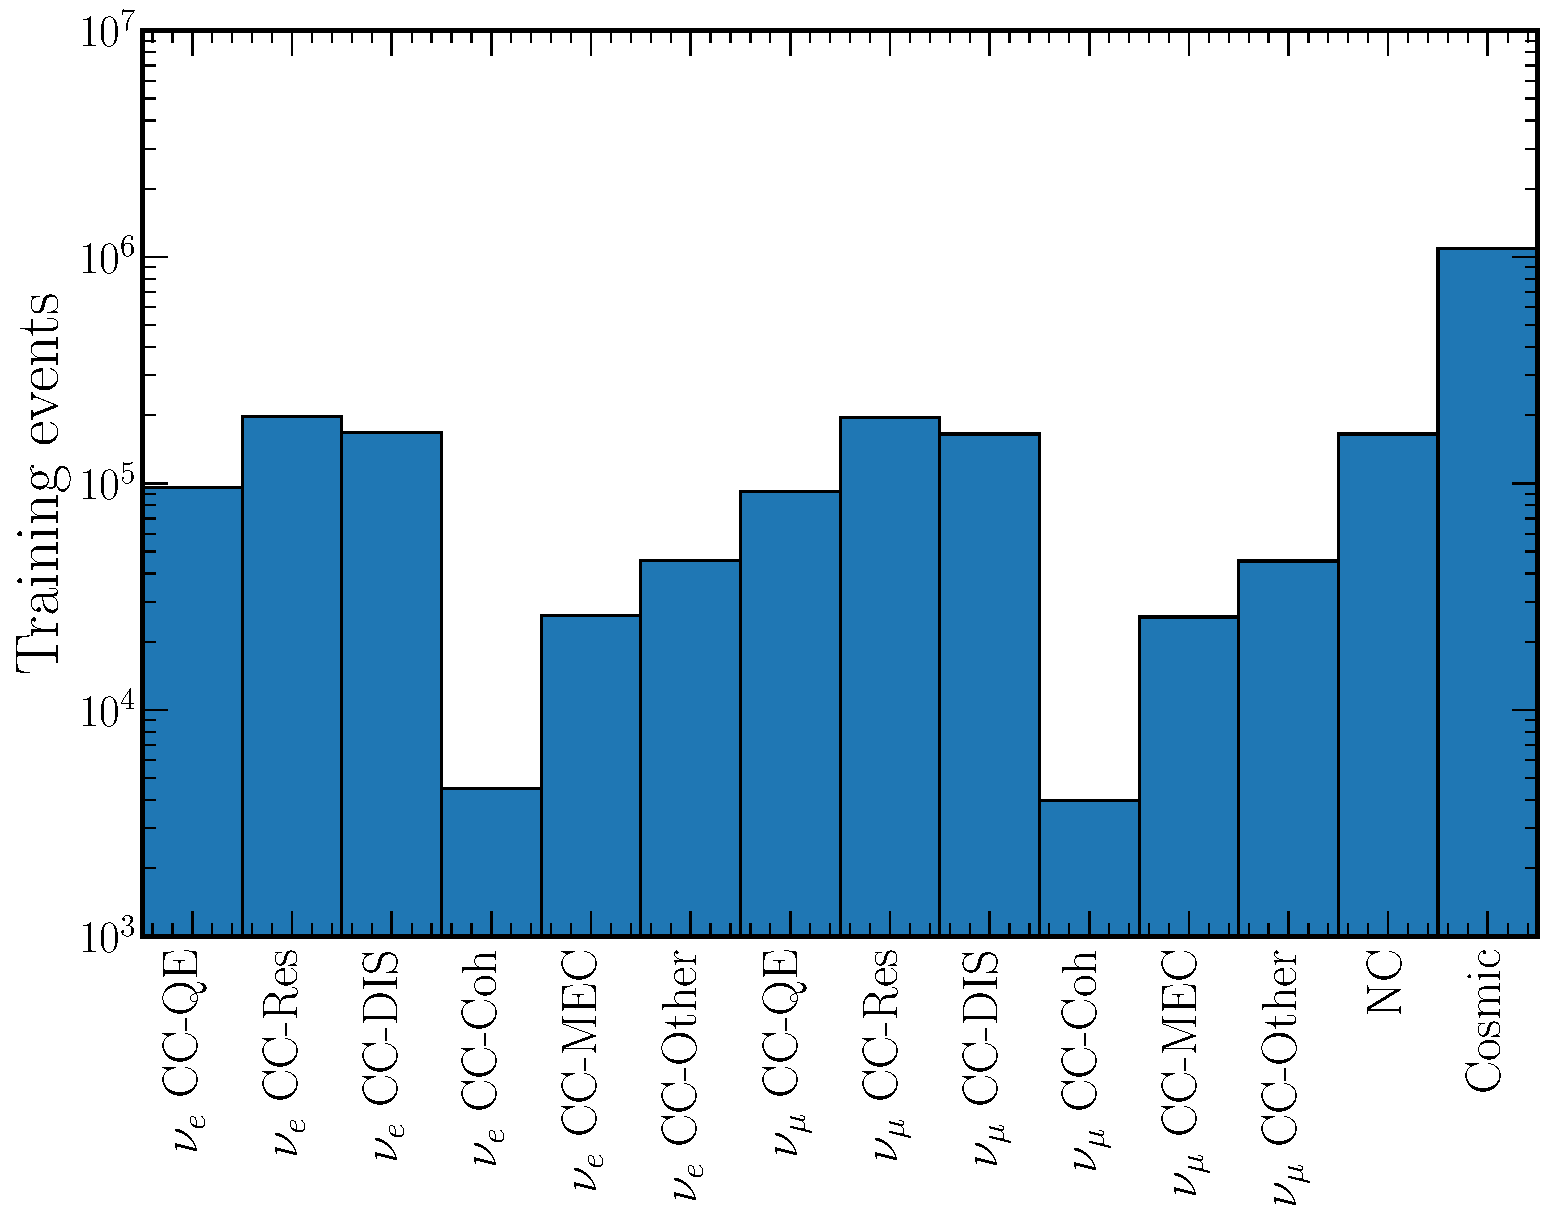
\includegraphics[width=0.6\textwidth]{diagrams/7-cvn/chipsnet/explore_t_nc_comb_cat.pdf}
    \caption[explore t nc comb cat short]
    {explore t nc comb cat long}
    \label{fig:explore_t_nc_comb_cat}
\end{figure}

\begin{figure} % T_COMB_CAT SAMPLE DIAGRAM %
    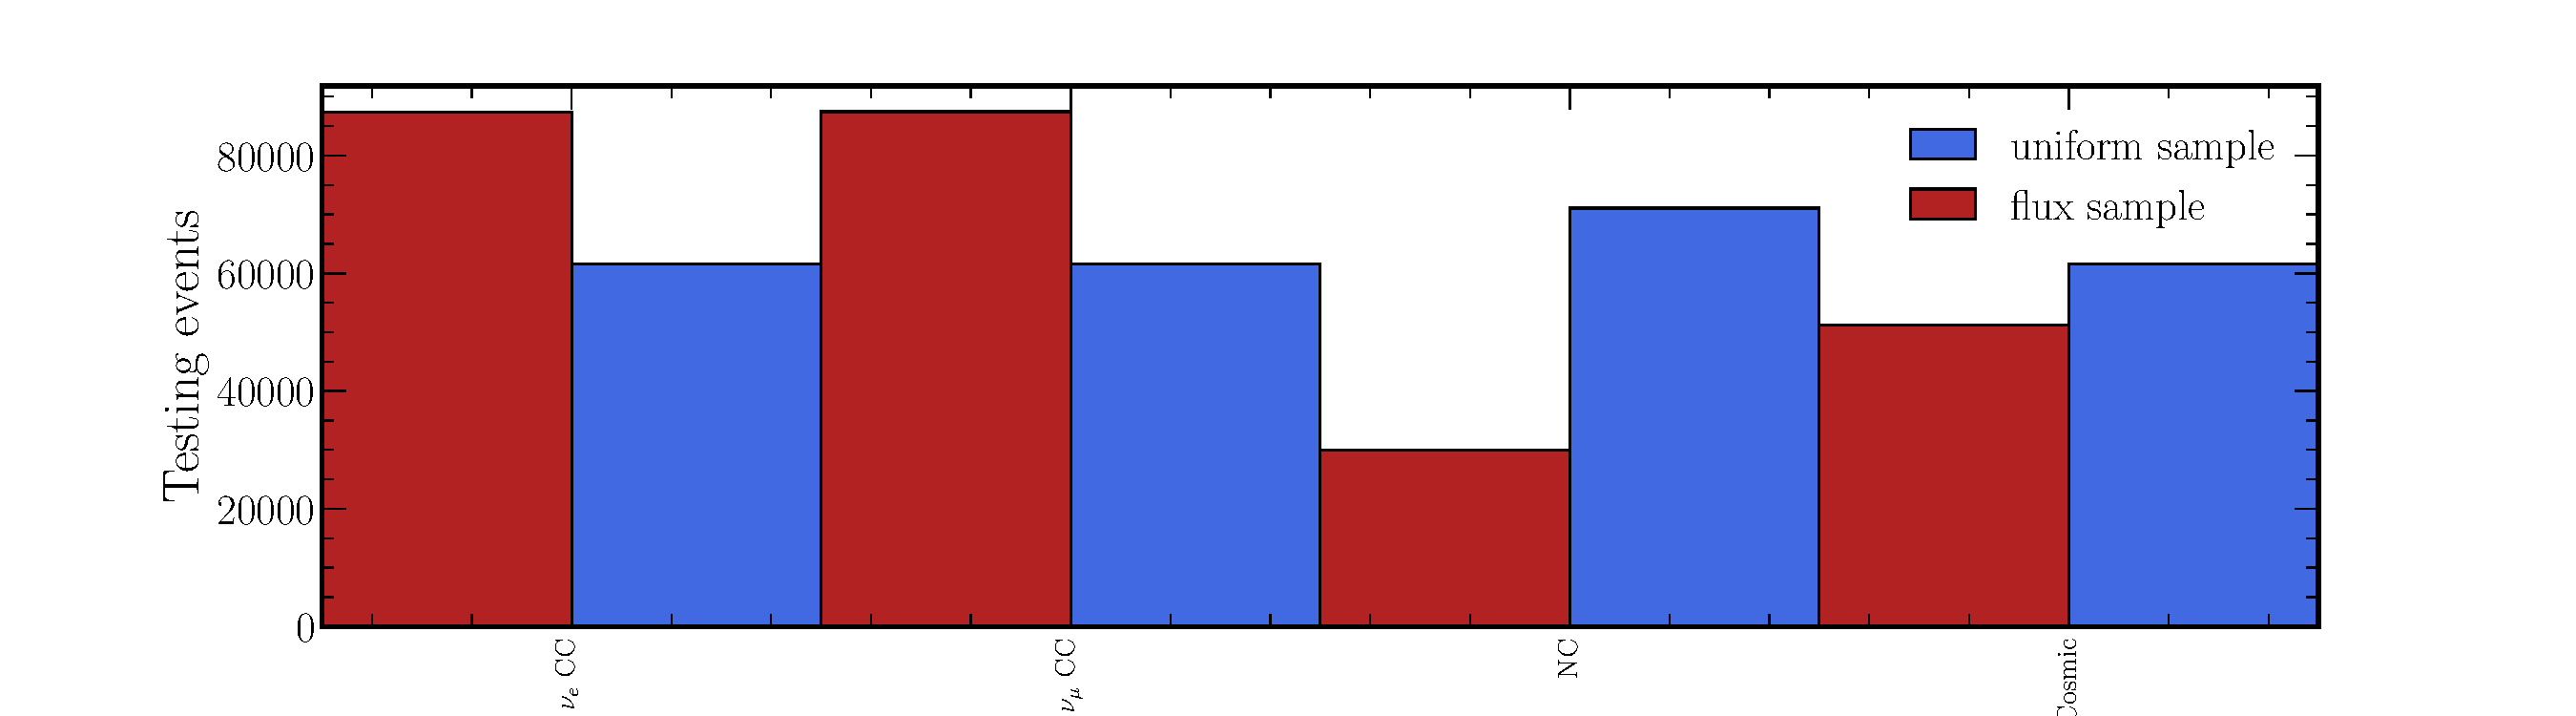
\includegraphics[width=0.6\textwidth]{diagrams/7-cvn/chipsnet/explore_t_comb_cat.pdf}
    \caption[explore t comb cat short]
    {explore t comb cat long}
    \label{fig:explore_t_comb_cat}
\end{figure}

\begin{figure} % CAT NUEL EFF CURVES DIAGRAM %
    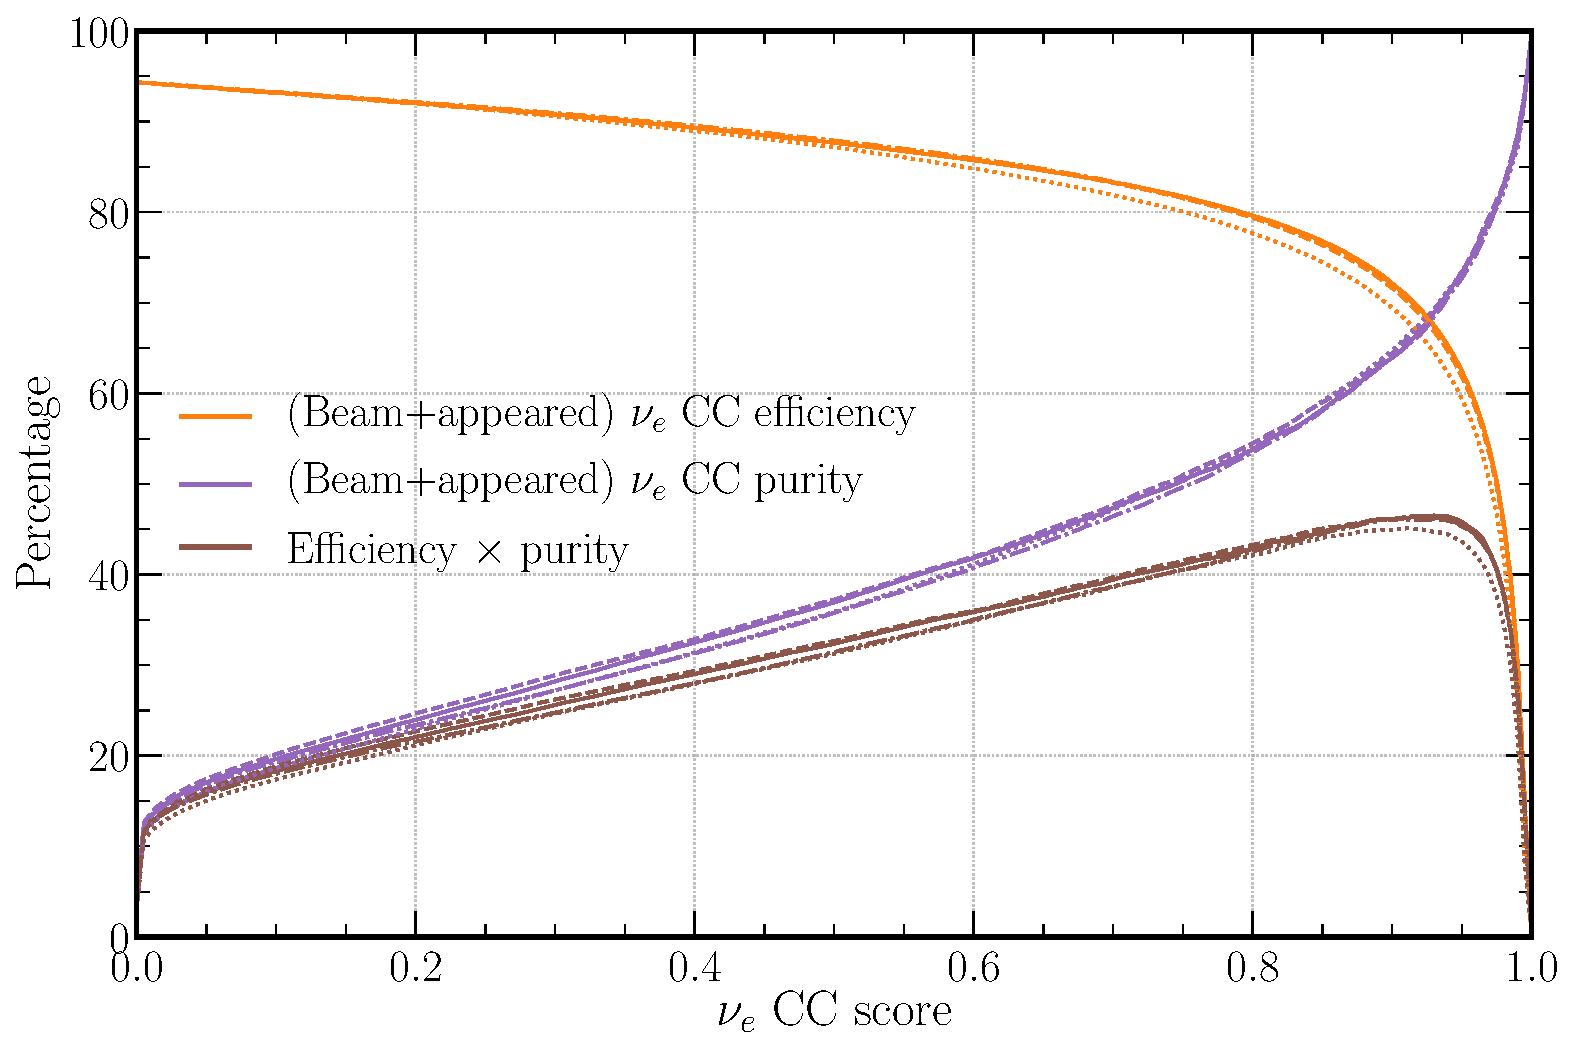
\includegraphics[width=0.6\textwidth]{diagrams/7-cvn/chipsnet/cat_nuel_eff_curves.pdf}
    \caption[cat nuel eff curves short]
    {cat nuel eff curves long}
    \label{fig:cat_nuel_eff_curves}
\end{figure}

\begin{figure} % CAT NUEL COMP CURVES DIAGRAM %
    \includegraphics[width=0.8\textwidth]{diagrams/7-cvn/chipsnet/cat_nuel_comp_curves.pdf}
    \caption[cat nuel comp curves short]
    {cat nuel comp curves long}
    \label{fig:cat_nuel_comp_curves}
\end{figure}

\begin{figure} % CAT NUMU EFF CURVES DIAGRAM %
    \includegraphics[width=0.6\textwidth]{diagrams/7-cvn/chipsnet/cat_numu_eff_curves.pdf}
    \caption[cat numu eff curves short]
    {cat numu eff curves long}
    \label{fig:cat_numu_eff_curves}
\end{figure}

\begin{figure} % CAT NUMU COMP CURVES DIAGRAM %
    \includegraphics[width=0.8\textwidth]{diagrams/7-cvn/chipsnet/cat_numu_comp_curves.pdf}
    \caption[cat numu comp curves short]
    {cat numu comp curves long}
    \label{fig:cat_numu_comp_curves}
\end{figure}

\subsection{Does counting primary particles help?} %%%%%%%%%%%%%%%%%%%%%%%%%%%%%%%%%%%%%%%%%%%%%%%
\label{sec:cvn_beam_prim} %%%%%%%%%%%%%%%%%%%%%%%%%%%%%%%%%%%%%%%%%%%%%%%%%%%%%%%%%%%%%%%%%%%%%%%%

- DUne tried counting exclusive final state particles (protons, chargedpions, neutral pions)
- As the different final states will have different energy resolutions and sytematic
uncertainties, it may be possible for a future analysis to improve the oscillation paramter
sensitivity by indentifying subsamples with specific topologies.
- Primary partile scores can be combined to give compounded scores for the exclusive final state
selections.

\begin{figure} % BEAM NUEL EFF CURVES DIAGRAM %
    \includegraphics[width=0.6\textwidth]{diagrams/7-cvn/chipsnet/beam_nuel_eff_curves.pdf}
    \caption[beam nuel eff curves short]
    {beam nuel eff curves long}
    \label{fig:beam_nuel_eff_curves}
\end{figure}

\begin{figure} % BEAM NUEL COMP CURVES DIAGRAM %
    \includegraphics[width=0.8\textwidth]{diagrams/7-cvn/chipsnet/beam_nuel_comp_curves.pdf}
    \caption[beam nuel comp curves short]
    {beam nuel comp curves long}
    \label{fig:beam_nuel_comp_curves}
\end{figure}

\begin{figure} % BEAM NUMU EFF CURVES DIAGRAM %
    \includegraphics[width=0.6\textwidth]{diagrams/7-cvn/chipsnet/beam_numu_eff_curves.pdf}
    \caption[beam numu eff curves short]
    {beam numu eff curves long}
    \label{fig:beam_numu_eff_curves}
\end{figure}

\begin{figure} % BEAM NUMU COMP CURVES DIAGRAM %
    \includegraphics[width=0.8\textwidth]{diagrams/7-cvn/chipsnet/beam_numu_comp_curves.pdf}
    \caption[beam numu comp curves short]
    {beam numu comp curves long}
    \label{fig:beam_numu_comp_curves}
\end{figure}

\section{Energy estimation} %%%%%%%%%%%%%%%%%%%%%%%%%%%%%%%%%%%%%%%%%%%%%%%%%%%%%%%%%%%%%%%%%%%%%%
\label{sec:cvn_energy} %%%%%%%%%%%%%%%%%%%%%%%%%%%%%%%%%%%%%%%%%%%%%%%%%%%%%%%%%%%%%%%%%%%%%%%%%%%

\subsection{Neutrino and lepton multitask} %%%%%%%%%%%%%%%%%%%%%%%%%%%%%%%%%%%%%%%%%%%%%%%%%%%%%%%
\label{sec:cvn_energy_chan} %%%%%%%%%%%%%%%%%%%%%%%%%%%%%%%%%%%%%%%%%%%%%%%%%%%%%%%%%%%%%%%%%%%%%%

\begin{figure} % ENERGY CHAN DISTS DIAGRAM %
    \includegraphics[width=\textwidth]{diagrams/7-cvn/chipsnet/energy_chan_frac_dist.pdf}
    \caption[energy chan frac dist short]
    {energy chan frac dist long}
    \label{fig:energy_chan_frac_dist}
\end{figure}

\begin{figure} % ENERGY CHAN FRAC VS E DIAGRAM %
    \includegraphics[width=\textwidth]{diagrams/7-cvn/chipsnet/energy_chan_frac_vs_e.pdf}
    \caption[energy chan frac vs e short]
    {energy chan frac vs e long}
    \label{fig:energy_chan_frac_vs_e}
\end{figure}

\subsection{Extra parameters} %%%%%%%%%%%%%%%%%%%%%%%%%%%%%%%%%%%%%%%%%%%%%%%%%%%%%%%%%%%%%%%%%%%%
\label{sec:cvn_energy_par} %%%%%%%%%%%%%%%%%%%%%%%%%%%%%%%%%%%%%%%%%%%%%%%%%%%%%%%%%%%%%%%%%%%%%%%

\begin{figure} % ENERGY PAR DISTS DIAGRAM %
    \includegraphics[width=\textwidth]{diagrams/7-cvn/chipsnet/energy_par_frac_dist.pdf}
    \caption[energy par frac dist short]
    {energy par frac dist long}
    \label{fig:energy_par_frac_dist}
\end{figure}

\begin{figure} % ENERGY PAR FRAC VS E DIAGRAM %
    \includegraphics[width=\textwidth]{diagrams/7-cvn/chipsnet/energy_par_frac_vs_e.pdf}
    \caption[energy par frac vs e short]
    {energy par frac vs e long}
    \label{fig:energy_par_frac_vs_e}
\end{figure}

\subsection{Combined or split} %%%%%%%%%%%%%%%%%%%%%%%%%%%%%%%%%%%%%%%%%%%%%%%%%%%%%%%%%%%%%%%%%%%
\label{sec:cvn_energy_split} %%%%%%%%%%%%%%%%%%%%%%%%%%%%%%%%%%%%%%%%%%%%%%%%%%%%%%%%%%%%%%%%%%%%%

\begin{figure} % ENERGY SPLIT NUEL DIAGRAM %
    \includegraphics[width=\textwidth]{diagrams/7-cvn/chipsnet/final_energy_split_nuel_frac_vs_e.pdf}
    \caption[final energy split nuel frac vs e short]
    {final energy split nuel frac vs e long}
    \label{fig:final_energy_split_nuel_frac_vs_e}
\end{figure}

\begin{figure} % ENERGY SPLIT NUMU DIAGRAM %
    \includegraphics[width=\textwidth]{diagrams/7-cvn/chipsnet/final_energy_split_numu_frac_vs_e.pdf}
    \caption[final energy split numu frac vs e short]
    {final energy split numu frac vs e long}
    \label{fig:final_energy_split_numu_frac_vs_e}
\end{figure}

\section{Combined performance} %%%%%%%%%%%%%%%%%%%%%%%%%%%%%%%%%%%%%%%%%%%%%%%%%%%%%%%%%%%%%%%%%%%
\label{sec:cvn_final} %%%%%%%%%%%%%%%%%%%%%%%%%%%%%%%%%%%%%%%%%%%%%%%%%%%%%%%%%%%%%%%%%%%%%%%%%%%%

\begin{figure} % COSMIC HISTORY DIAGRAM %
    \includegraphics[width=0.6\textwidth]{diagrams/7-cvn/chipsnet/final_cosmic_history.pdf}
    \caption[final cosmic history short]
    {final cosmic history long}
    \label{fig:final_cosmic_history}
\end{figure}

\begin{figure} % BEAM HISTORY DIAGRAM %
    \includegraphics[width=0.6\textwidth]{diagrams/7-cvn/chipsnet/final_beam_history.pdf}
    \caption[final beam history short]
    {final beam history long}
    \label{fig:final_beam_history}
\end{figure}

\begin{figure} % ENERGY HISTORY DIAGRAM %
    \includegraphics[width=0.6\textwidth]{diagrams/7-cvn/chipsnet/final_energy_history.pdf}
    \caption[final energy history short]
    {final energy history long}
    \label{fig:final_energy_history}
\end{figure}

\begin{figure} % COSMIC OUTPUTS DIAGRAM %
    \includegraphics[width=0.6\textwidth]{diagrams/7-cvn/chipsnet/final_cosmic_outputs.pdf}
    \caption[final cosmic outputs short]
    {final cosmic outputs long}
    \label{fig:final_cosmic_outputs}
\end{figure}

\begin{figure} % COSMIC OUTPUTS ZOOMED DIAGRAM %
    \includegraphics[width=0.6\textwidth]{diagrams/7-cvn/chipsnet/final_cosmic_zoomed_outputs.pdf}
    \caption[final cosmic zoomed outputs short]
    {final cosmic zoomed outputs long}
    \label{fig:final_cosmic_zoomed_outputs}
\end{figure}

\begin{figure} % ESCAPES OUTPUTS DIAGRAM %
    \includegraphics[width=0.6\textwidth]{diagrams/7-cvn/chipsnet/final_escapes_outputs.pdf}
    \caption[final escapes outputs short]
    {final escapes outputs long}
    \label{fig:final_escapes_outputs}
\end{figure}

\begin{figure} % BEAM OUTPUTS NUEL DIAGRAM %
    \includegraphics[width=0.6\textwidth]{diagrams/7-cvn/chipsnet/final_beam_nuel_outputs.pdf}
    \caption[final beam nuel outputs short]
    {final beam nuel outputs long}
    \label{fig:final_beam_nuel_outputs}
\end{figure}

\begin{figure} % BEAM OUTPUTS NUMU DIAGRAM %
    \includegraphics[width=0.6\textwidth]{diagrams/7-cvn/chipsnet/final_beam_numu_outputs.pdf}
    \caption[final beam numu outputs short]
    {final beam numu outputs long}
    \label{fig:final_beam_numu_outputs}
\end{figure}

\begin{figure} % FINAL NUEL EFF CURVES DIAGRAM %
    \includegraphics[width=0.6\textwidth]{diagrams/7-cvn/chipsnet/final_nuel_eff_curves.pdf}
    \caption[final nuel eff curves short]
    {final nuel eff curves long}
    \label{fig:final_nuel_eff_curves}
\end{figure}

\begin{figure} % FINAL NUMU EFF CURVES DIAGRAM %
    \includegraphics[width=0.6\textwidth]{diagrams/7-cvn/chipsnet/final_numu_eff_curves.pdf}
    \caption[final numu eff curves short]
    {final numu eff curves long}
    \label{fig:final_numu_eff_curves}
\end{figure}

\begin{figure} % FINAL NUEL HISTS DIAGRAM %
    \includegraphics[width=0.6\textwidth]{diagrams/7-cvn/chipsnet/final_nuel_hists.pdf}
    \caption[final nuel hists short]
    {final nuel hists long}
    \label{fig:final_nuel_hists}
\end{figure}

\begin{figure} % FINAL NUMU HISTS DIAGRAM %
    \includegraphics[width=0.6\textwidth]{diagrams/7-cvn/chipsnet/final_numu_hists.pdf}
    \caption[final numu hists short]
    {final numu hists long}
    \label{fig:final_numu_hists}
\end{figure}

\begin{figure} % FINAL COMB CAT CONFUSION DIAGRAM %
    \includegraphics[width=0.6\textwidth]{diagrams/7-cvn/chipsnet/final_comb_cat_confusion.pdf}
    \caption[final comb cat confusion short]
    {final comb cat confusion long}
    \label{fig:final_comb_cat_confusion}
\end{figure}

\begin{figure} % FINAL CC CAT CONFUSION DIAGRAM %
    \includegraphics[width=0.6\textwidth]{diagrams/7-cvn/chipsnet/final_cc_cat_confusion.pdf}
    \caption[final cc cat confusion short]
    {final cc cat confusion long}
    \label{fig:final_cc_cat_confusion}
\end{figure}

\begin{figure} % FINAL NC CAT CONFUSION DIAGRAM %
    \includegraphics[width=0.6\textwidth]{diagrams/7-cvn/chipsnet/final_nc_cat_confusion.pdf}
    \caption[final nc cat confusion short]
    {final nc cat confusion long}
    \label{fig:final_nc_cat_confusion}
\end{figure}

\begin{figure} % FINAL NUEL ENERGY DIST DIAGRAM %
    \includegraphics[width=0.6\textwidth]{diagrams/7-cvn/chipsnet/final_nuel_passed_energy_dist.pdf}
    \caption[final nuel passed energy dist short]
    {final nuel passed energy dist long}
    \label{fig:final_nuel_passed_energy_dist}
\end{figure}

\begin{figure} % FINAL NUMU ENERGY DIST DIAGRAM %
    \includegraphics[width=0.6\textwidth]{diagrams/7-cvn/chipsnet/final_numu_passed_energy_dist.pdf}
    \caption[final numu passed energy dist short]
    {final numu passed energy dist long}
    \label{fig:final_numu_passed_energy_dist}
\end{figure}

\begin{figure} % FINAL 2D ENERGY DIAGRAM %
    \includegraphics[width=0.7\textwidth]{diagrams/7-cvn/chipsnet/final_energy_2d.pdf}
    \caption[final energy 2d short]
    {final energy 2d long}
    \label{fig:final_energy_2d}
\end{figure}

\begin{figure} % FINAL NUEL ENERGY DIAGRAM %
    \includegraphics[width=0.8\textwidth]{diagrams/7-cvn/chipsnet/final_energy_nuel.pdf}
    \caption[final energy nuel short]
    {final energy nuel long}
    \label{fig:final_energy_nuel}
\end{figure}

\begin{figure} % FINAL NUMU ENERGY DIAGRAM %
    \includegraphics[width=0.8\textwidth]{diagrams/7-cvn/chipsnet/final_energy_numu.pdf}
    \caption[final energy numu short]
    {final energy numu long}
    \label{fig:final_energy_numu}
\end{figure}

DIAGRAM: True neutrino energy distributions for different categories for energy estimation.
DIAGRAM: Neutrino energy and estimated neutrino energy distributions on same plots.
INFO: Table of the final number of expected events and efficiency and purity of the signal at the
chosen cut value (nuel and numu)
DIAGRAM: Parrallel coordinates plots for tuning the hyperparameters
INFO: Time taken comparison with old reconstruction (just inference time for all stages)
INFO: Super-k/Dune/Nova comparison numbers for effeciencies and energy resolutions etc...
DIAGRAM: Table of how succesive cuts affect the selection of different event types
DIAGRAM: Plots of exclusive state predictions by multiplying different score outputs.

- BIG UP the difference in time it takes, as this can have a huge impact on reprocessing your full
dataset
- This allows a massive increase in the iteration rate of analysis, which can lead to an improved
rate of improvement, with less time wasted.

INFO: Need to understand the error on the number of cosmic passing the cut, is it reasonable
without a huge amount of testing data?
INFO: What are the errors on all my number values? with the stats I have?
- Having a veto in the upstream towards the beam direction would be best
- Talk about how beam muons upstream of the detector are just like cosmics and say how they could
be rejected aswell
INFO: proof that there is no topological difference between QEL and MEC if we are combining them
for the energy stuff
- Position of PMTs does not seem to be that important

- Nova gets about ~7percent energy resolution for signal events
in Ref.~\cite{jiang2019}
- Fitqun gets ~20cm vertex position resolution for nuel CCQE events
- Fitqun gets ~16cm vertex position resolution for numu CCQE events
- Fitqun gets 5.39percent to 2.58percent lepton energy resolution for nuel CCQE events
- Fitqun gets ~2.5percent lepton energy resolution for numu CCQE events
- Note all the stuff in super-k happens at lower energies ~<1.4GeV

\section{Explainability} %%%%%%%%%%%%%%%%%%%%%%%%%%%%%%%%%%%%%%%%%%%%%%%%%%%%%%%%%%%%%%%%%%%%%%%%%
\label{sec:cvn_explain} %%%%%%%%%%%%%%%%%%%%%%%%%%%%%%%%%%%%%%%%%%%%%%%%%%%%%%%%%%%%%%%%%%%%%%%%%%

\begin{figure} % COSMIC t-SNE DIAGRAM %
    \includegraphics[width=0.8\textwidth]{diagrams/7-cvn/chipsnet/final_cosmic_tsne.pdf}
    \caption[final cosmic tsne short]
    {final cosmic tsne long}
    \label{fig:final_cosmic_tsne}
\end{figure}

\begin{figure} % BEAM t-SNE DIAGRAM %
    \includegraphics[width=0.8\textwidth]{diagrams/7-cvn/chipsnet/final_beam_tsne.pdf}
    \caption[final beam tsne short]
    {final beam tsne long}
    \label{fig:final_beam_tsne}
\end{figure}

\begin{figure} % BEAM t-SNE EVENTS DIAGRAM %
    \includegraphics[width=\textwidth]{diagrams/7-cvn/chipsnet/final_beam_tsne_events.pdf}
    \caption[final beam tsne events short]
    {final beam tsne events long}
    \label{fig:final_beam_tsne_events}
\end{figure}

\begin{figure} % FRAC ENERGY EFF DIAGRAM %
    \includegraphics[width=0.6\textwidth]{diagrams/7-cvn/chipsnet/final_frac_energy_eff.pdf}
    \caption[final frac energy eff short]
    {final frac energy eff long}
    \label{fig:final_frac_energy_eff}
\end{figure}

\begin{figure} % EXPLAIN EXAMPLE EVENT DIAGRAM %
    \includegraphics[width=\textwidth]{diagrams/7-cvn/chipsnet/explain_example_event.pdf}
    \caption[explain example event short]
    {explain example event long}
    \label{fig:explain_example_event}
\end{figure}

\begin{figure} % BEAGLEBONE AND DANOUT DIAGRAM %
    \centering
    \subcaptionbox{explain cosmic activations\label{fig:explain_cosmic_activations}}{%
        \includegraphics[height=16cm]{diagrams/7-cvn/chipsnet/explain_cosmic_activations.pdf}%
    }
    \quad
    \subcaptionbox{explain beam activations\label{fig:explain_beam_activations}}{%
        \includegraphics[height=16cm]{diagrams/7-cvn/chipsnet/explain_beam_activations.pdf}%
    }
    \quad
    \subcaptionbox{explain energy activations\label{fig:explain_energy_activations}}{%
        \includegraphics[height=16cm]{diagrams/7-cvn/chipsnet/explain_energy_activations.pdf}%
    }
    \caption[The caption]
    {The caption}
\end{figure}

Initial CNN visualisation paper in Ref.~\cite{zeiler2013}
Original t-SNE paper in Ref.~\cite{maaten2008}
Grad-CAM paper in Ref.~\cite{selvaraju2017}

- For all the t-SNE stuff
- There have been plently of attempts at visualising high-dimensional data on a 2/3 dimensional
map, including Sammon mapping, Isomap, Locally Linear Embedding, Stochastic Neighbour Embedding.
- Older implementations tended to cluster all data points towards the centre of the map and proved
difficult to optimise.
- You basically set a summed probability between all points in the low-dimensional space to a
summed probability between all points in the high-dimensional space.
- t-SNE uses the student-t distribution (with a heavy tail) in the low-dimensional space to
calculate the probability. This alleviates both the crowding problem and is easier to optimise.
- Optimisation uses a simple momentum term, plus two new ideas. "Early compression" which forces
map points to stay close to each other at the start of optimisation, it is then easier for
clusters to move through each other and explore all possible global organisations of the data,
this is implemented as an L2-penalty term proportional to the sum of squared distances from the
origin, this is then removed at an iteration given as input. Secondly, "Early exaggeration" which
creates tight widely seperated clusters.